% ============= Package Einstellungen & Sonstiges ============= 
\documentclass[a4paper,12pt]{report}
\usepackage[left= 2.5 cm,right = 2.5 cm, bottom = 2.5 cm]{geometry}
\usepackage[onehalfspacing]{setspace}

\usepackage[
pdftitle={Studienarbeit},
pdfsubject={Entwicklung einer smarten Bewässerungslösung mit Web-Anbindung},
pdfauthor={Maximilian Schüller, Fynn Thierling, Justus Siegert, Lukas Maier, Timon Kleinknecht},
pdfkeywords={},	
hidelinks %Links nicht einrahmen
]{hyperref}

\usepackage[utf8]{inputenc}
\usepackage[ngerman]{babel}
\usepackage[T1]{fontenc}

\usepackage{fancyhdr}
\usepackage{color}
\usepackage{csquotes}
%\usepackage{cite}
\usepackage[backend=biber, autocite=inline, style=ieee, natbib=true]{biblatex}
\addbibresource{literatur.bib}
\DefineBibliographyStrings{ngerman}{andothers = {{et\,al\adddot}},}
\usepackage{url}

\usepackage{graphicx} %für Einbindung von Grafiken
\graphicspath{{img/}} %Pfad für Grafiken
\usepackage{svg}
\usepackage{amsmath}

\usepackage{pdfpages}

\usepackage{todonotes}

%\usepackage[printonlyused]{acronym}
% Akronymverzeichnis
\usepackage{hyperref}
\usepackage{array}
\usepackage{supertabular}
\usepackage{acro}
\acsetup{make-links}
%Überschrift "Abkürzungsverzeichnis" setzen
\section*{Abkürzungsverzeichnis}
\addcontentsline{toc}{section}{Abkürzungsverzeichnis}
\begin{acronym}[STRIDE]
	%\acro{EXP}{example}	-> Im text verwenden mit \ac{EXP}	
	
\end{acronym}

\usepackage{minted} %für Darstellung von Code
\usepackage{float}
\usepackage[german]{varioref} %für schönere Referenzierung von Abbildungen

\fancyhead[L]{} % Linke Kopfzeile leer lassen

\usepackage{xspace}

% Define a command to ensure consistent space after acronym
%\newcommand{\acspace}{\xspace\hspace{1em}}

\makeatletter
%\renewcommand*{\aclabelfont}[1]{\textbf{\acsfont{#1}\acspace}}
\makeatother


\newcommand{\source}[1]{\vspace{1ex}\noindent{\small \textit{Quelle: #1}}}
\newcommand{\file}[1]{\texttt{#1}}
\DeclareUnicodeCharacter{202F}{\%}

\newcommand{\initializeBibliography}{
	\ihead{}
	\printbibliography[title=\Literaturverzeichnis] 
	\cleardoublepage
}

\usepackage{enumitem}
\usepackage{amssymb}

\usepackage{listings}
\usepackage{listings-golang}
\usepackage{xcolor}  % Optional, für zusätzliche Farbanpassungen
\lstset{ 
	language=Python,                % Programmiersprache
	basicstyle=\ttfamily\scriptsize,     % Grundschriftart (monospace) und -größe
	keywordstyle=\bfseries\color{blue}, % Schlüsselwörter fett und blau
	commentstyle=\itshape\color{green!50!black}, % Kommentare kursiv und grün
	stringstyle=\color{red},        % Strings rot
	numbers=left,                   % Zeilennummern links anzeigen
	numberstyle=\tiny\color{black},  % Stil der Zeilennummern (klein und grau)
	stepnumber=1,                   % Jede Zeile nummerieren
	numbersep=8pt,                  % Abstand der Zeilennummern zum Code
	backgroundcolor=\color{gray!10},  % Hintergrundfarbe des Codes (weiß)
	frame=single,                   % Rahmen um den Code
	rulecolor=\color{black},        % Rahmenfarbe
	captionpos=b,                   % Position des Titels (unten)
	breaklines=true,                % Zeilen umbrechen, wenn sie zu lang sind
	breakatwhitespace=true,         % Zeilenumbrüche nur an Leerzeichen
	showstringspaces=false,         % Leerzeichen in Strings nicht anzeigen
	tabsize=4,                      % Breite eines Tabs
	%escapeinside={(*@}{@*)},        % LaTeX-Befehle innerhalb des Codes
	morekeywords={print,def,class}, % Zusätzliche Schlüsselwörter für Python
	extendedchars=true,             % Unterstützt erweiterte Zeichen (z. B. Umlaute)
}
% Label für Listings ändern
\renewcommand{\lstlistingname}{Beispiel}
\newcommand{\code}[1]{\colorbox{gray!20}{\consola #1}}

\usepackage{titlesec}
\titleformat{\chapter}[hang]
  {\normalfont\huge\bfseries}
  {\thechapter\quad}
  {0pt}
  {} 


% ============= Dokumentbeginn =============
\begin{document}
	
	%Titelseite
	\thispagestyle{empty}
\begin{center}
\begin{tabular}{p{\textwidth}}
		
\begin{center}
	\textbf{\Large{\textsc{
			Entwicklung einer smarten Bewässerungslösung mit Web-Anbindung
	}}}
\end{center}

\vspace{1em}
\vspace{1em}
\vspace{1em}

\begin{center}
	\Large{Studienarbeit}
\end{center}

\vspace{1em}

\begin{center}
	im Rahmen des \\
	\large{\textbf{Bachelor of Science (B.Sc.)}} 
\end{center}

\vspace{1em}

\begin{center}
	des Studiengangs Informatik Cyber Security \\
	der Dualen Hochschule Baden-Württemberg Mannheim
\end{center}

\vspace{1em}
\vspace{1em}

\begin{center}
	vorgelegt von
\end{center}

\begin{center}
	\textbf{Maximilian Schüller, Fynn Thierling, Justus Siegert,\\Lukas Maier, Timon Kleinknecht}
\end{center}

\vspace{1em}
\vspace{1em}

\begin{center}
	\today
\end{center}
\end{tabular}
\end{center}
	
	\cleardoublepage
	\pagenumbering{roman}
	
	%------------- Erklärung der Eigenleistung-----------

	\pagebreak
\hspace{0pt}
\vfill
\begin{center}
    \large{Erklärung der Eigenleistung}
\end{center}
\vspace{1em}
\begin{center}
    \textit{Hiermit erklären wir, dass wir die vorliegende Studienarbeit selbstständig und ohne fremde Hilfe verfasst haben. Wir haben keine anderen als die angegebenen Quellen und Hilfsmittel benutzt. Darüber hinaus erklären wir, dass im Rahmen des Schreibprozesses KI-gestützte Werkzeuge (ChatGPT) zur Umformulierung von Textstellen verwendet wurden. Wir bestätigen hiermit, dass alle verwendeten Quellenangaben korrekt sind und die inhaltliche Verantwortung für die Arbeit uneingeschränkt bei uns liegt.}
\end{center}

\begin{tabular}{>{\centering\arraybackslash}p{0.5\textwidth} >{\centering\arraybackslash}p{0.5\textwidth}}
  \includegraphics[height=2\baselineskip, keepaspectratio]{img/MS_Unterschrift.png}
  &
  \includegraphics[height=2\baselineskip, keepaspectratio]{img/FT_Unterschrift.png}
  \\
  Maximilian Schüller & Fynn Thierling \\
  \includegraphics[height=2\baselineskip, keepaspectratio]{img/JS_Unterschrift.png}
  &
  \includegraphics[height=2\baselineskip, keepaspectratio]{img/LM_Unterschrift.jpg}
  \\
  Justus Siegert & Lukas Maier \\
  \includegraphics[height=2\baselineskip, keepaspectratio]{img/Unterschrift_TK.jpg}
  &
  \\
  Timon Kleinknecht & Mannheim, 15.04.2025
\end{tabular}


\vfill
\hspace{0pt}
\pagebreak

	\newpage

	%------------- Abstract -------------
	% Abstract in English
\section*{Abstract}
\addcontentsline{toc}{section}{Abstract}

\newpage

% Abstract in Deutsch
\section*{Abstrakt}
\addcontentsline{toc}{section}{Abstrakt}


	\newpage
	
	%------------- Inhaltsverzeichnis -------------
	\tableofcontents
	
	%------------- Abkürzungsverzeichnis -------------
	%%Überschrift "Abkürzungsverzeichnis" setzen
\section*{Abkürzungsverzeichnis}
\addcontentsline{toc}{section}{Abkürzungsverzeichnis}
\begin{acronym}[STRIDE]
	%\acro{EXP}{example}	-> Im text verwenden mit \ac{EXP}	
	
\end{acronym}
	\printacronyms[template=supertabular]
    \addcontentsline{toc}{chapter}{Abkürzungen}
    \newpage
	
	%------------- Abbildungsverzeichnis -------------
	\section*{Abbildungsverzeichnis}
	\addcontentsline{toc}{section}{Abbildungsverzeichnis}
	\renewcommand{\listfigurename}{} % Verhindert doppelten großen Titel
	\newpage

	
	%------------- Tabellenverzeichnis -------------
	\section*{\listtablename}
	\addcontentsline{toc}{section}{\listtablename}
	\renewcommand{\listtablename}{} % Verhindert doppelten großen Titel
	\newpage

	
	% pagestyle für restliches Dokument aktivieren
	\pagestyle{fancy}
	\pagenumbering{arabic}
	


	%------------- Einleitung -------------
	\chapter{Einleitung}
	\section{Motivation}
\label{sec:Motivation}

Pflanzen gehören in Deutschland und Europa fest zum Alltag in Wohnung und Garten. Laut einer repräsentativen Umfrage aus dem Jahr 2020 besitzen rund drei Viertel der Bundesbürger:innen (74\,\%) Zimmerpflanzen in ihrem Zuhause; auch auf Balkonen (35\,\%), Terrassen (30\,\%) und Fensterbänken (21\,\%) grünt es, während nur etwa 10\,\% ganz ohne Pflanzen leben\autocite{pflanzenbesitz_de}. Dieses „grüne Zuhause“ liegt im Trend und gewann insbesondere während der COVID-19-Pandemie an Bedeutung – viele Menschen entdeckten 2020 im Home-Office ihre Liebe zu Haus- und Gartenpflanzen neu\autocite{pflanzenbesitz_de}. Entsprechend stieg der Absatz: Der deutsche Markt für Blumen und Zierpflanzen erreichte nach Jahren der Stagnation 2020 ein Rekordvolumen von 9{,}4\,Mrd.\,€\autocite{stihl_gartenbarometer}. Ähnlich hohe Werte zeigen sich europaweit, wo Pflanzen als wichtiger Teil der Wohn- und Lebensqualität gelten. Neben dekorativen Aspekten werden Zimmer- und Gartenpflanzen aufgrund positiver Effekte wie besserer Luftqualität und Stressreduktion geschätzt\autocite{pflanzenbesitz_de}. Die hohe Verbreitung und Wertschätzung von Pflanzen in Privathaushalten bildet den Ausgangspunkt für die Betrachtung, wie ihre Pflege im Alltag unterstützt werden kann.

Allerdings stehen viele Pflanzenbesitzer:innen vor praktischen Herausforderungen bei der Pflege ihres „grünen Mitbewohners“. Im hektischen Alltag wird das Gießen leicht vergessen oder unregelmäßig vorgenommen; umgekehrt gießen unerfahrene Halter oft zu viel aus Sorge um die Pflanze. Studien bestätigen, dass Überwässerung der häufigste Grund für das Eingehen von Zimmerpflanzen ist\autocite{pflanzenpflege_fehler}. Generell erfordert jede Pflanzenart spezifische Kenntnisse zu Wasser- und Nährstoffbedarf, Lichtverhältnissen etc., über die im privaten Umfeld nicht immer ausreichend Wissen vorhanden ist. So gaben in einer Umfrage lediglich 37\,\% der befragten Frauen und 20\,\% der Männer an, einen „grünen Daumen“ zu haben\autocite{pflanzenbesitz_de} – die Mehrheit traut sich die optimale Pflanzenpflege also eher nicht zu. Hinzu kommt, dass während Urlaubs- oder Abwesenheitszeiten oft keine Betreuung für die heimischen Gewächse sichergestellt ist. Tatsächlich vermissten in einer Befragung 26\,\% der Pflanzenhalter:innen ihre Zimmerpflanzen im Urlaub sogar mehr als die Kolleg:innen\autocite{pflanzenbesitz_de}, was die emotionale Bindung und zugleich das Problem der Versorgung in dieser Zeit verdeutlicht. Diese Pflegeherausforderungen führen dazu, dass viele privat gehaltene Pflanzen Schäden nehmen oder vorzeitig absterben.

Die Folgen von falscher oder unregelmäßiger Pflege sind in Zahlen beträchtlich. Hochrechnungen zufolge überlebt ein erheblicher Teil der gekauften Zierpflanzen nicht lange: Etwa 40\,\% der Pflanzen gehen bereits in der Lieferkette zugrunde, und weitere rund 35\,\% sterben später in den Wohnungen der Kundschaft\autocite{pflanzensterben_statistik}. Mit anderen Worten wird fast die Hälfte aller gekauften Haus- und Gartenpflanzen letztlich aufgrund suboptimaler Bedingungen oder Pflegefehler nicht dauerhaft erhalten. Auch Verbraucherumfragen deuten auf dieses Problem hin. Beispielsweise gab über ein Drittel der Hobbygärtner in einer aktuellen Erhebung an, jedes Jahr ein bis zwei Zimmerpflanzen zu verlieren\autocite{pflanzensterben_statistik}. Solche Verluste sind nicht nur emotional enttäuschend für Pflanzenliebhaber, sondern bedeuten auch Ressourcenverschwendung – insbesondere von Wasser, Zeit und Geld. Schätzungen aus den USA zeigen etwa, dass jüngere „Plant Parents“ im Durchschnitt schon mehrere ihrer erworbenen Pflanzen unbeabsichtigt zum Eingehen gebracht haben. Diese Zahlen unterstreichen die Notwendigkeit, neue Wege zu finden, um häufige Pflegefehler zu vermeiden und die Lebensdauer der Pflanzen zu verlängern.

Technologische Lösungen im Sinne von \textit{Smart Gardening} setzen hier an und versprechen Abhilfe. Insbesondere automatische Bewässerungssysteme für den Heimgebrauch bieten die Möglichkeit, den Gießvorgang zu optimieren und zu automatisieren. Solche Systeme kombinieren oft Sensoren (etwa für Bodenfeuchte oder Licht) mit internetfähigen Steuerungen, um den Pflanzen exakt bei Bedarf und in der richtigen Menge Wasser zuzuführen. Erste Ansätze sind bereits auf dem Markt verfügbar – von App-gesteuerten Bewässerungscomputern bis hin zu smarten Pflanzentöpfen mit Selbstbewässerungs-Funktion. Die Akzeptanz solcher \textit{Smart-Home}-Technologien im Garten- und Pflanzenbereich steigt kontinuierlich. Laut dem STIHL-Gartenbarometer 2022 nutzen bereits rund 7\,\% der deutschen Gartenbesitzer smarte Garden-Lösungen, und etwa 30\,\% wünschen sich zukünftig solche automatisierten Helfer\autocite{stihl_gartenbarometer}. Dabei stehen Bewässerungsautomationen an erster Stelle der Wunschliste: 83\,\% der Befragten mit Smart-Gardening-Interesse nennen ein automatisches Bewässerungssystem als besonders gefragte Lösung. Diese Nachfrage spiegelt sich auch in anderen Ländern wider. Beispielsweise glauben in Österreich über 60\,\% der Gartenbesitzer, dass sich der Wasserverbrauch durch automatisierte Bewässerungsanlagen deutlich optimieren lässt. Moderne Systeme können Wetterdaten oder Bodensensoren einbeziehen, um nur dann zu wässern, wenn die Pflanze es wirklich benötigt – eine Technik, die den Pflanzenstress reduziert und zugleich Wasserverschwendung vorbeugt. Aktuelle Untersuchungen zeigen denn auch, dass intelligente Bewässerungssteuerungen den Wasserverbrauch im Garten gegenüber herkömmlichen Timern erheblich senken können (um etwa 20–40\,\% je nach System).

Mehrere übergeordnete Trends begünstigen die Verbreitung von smarten Pflanzenpflege-Systemen. Zum einen führt die Urbanisierung dazu, dass immer mehr Menschen auf kleinem Raum in Städten leben – in Deutschland etwa 78\,\% der Bevölkerung\autocite{urbanisierung_de} – und sich dennoch nach Natur im eigenen Umfeld sehnen. Insbesondere Stadtbewohner ohne Garten kultivieren vermehrt Zimmerpflanzen oder Balkongrün, sind aber beruflich oft stark eingebunden. Eine automatische Bewässerung kann hier den Pflegeaufwand mindern und sicherstellen, dass Pflanzen trotz hektischem Alltag oder Abwesenheiten ausreichend versorgt werden. Zum anderen rückt Nachhaltigkeit in den Fokus: Wassermanagement und effiziente Ressourcennutzung gewinnen an Bedeutung, da die Auswirkungen des Klimawandels – etwa häufigere Sommerdürreperioden – auch private Gärten und Balkone betreffen. In Umfragen äußern fast zwei Drittel der Befragten die Erwartung, dass digitale Technologien im Garten helfen können, den Klimawandel abzuschwächen, und nennen den schonenden Umgang mit Wasser als oberste Priorität. Smart-Bewässerungssysteme erfüllen genau diesen Zweck, indem sie bedarfsgerecht gießen und Überwässerung verhindern. Schließlich trägt auch die allgemeine Verbreitung von \textit{Internet of Things}-Anwendungen im Haushalt dazu bei, dass vernetzte Lösungen immer selbstverständlicher werden. Der europäische Smart-Home-Markt verzeichnet hohe Wachstumsraten und wird 2024 bereits auf über 22\,Mrd.\,US-\$ geschätzt\autocite{iot_trend}. Vernetzte, per App oder Sprache steuerbare Geräte – vom Thermostat bis zur Lichtsteuerung – gehören zunehmend zum Alltag. Diese Entwicklung macht auch vor dem Bereich der Pflanzenpflege nicht Halt: Die Nutzerakzeptanz für digitale Helfer im Haushalt schafft ein günstiges Umfeld für \textit{Smart Gardening}-Innovationen.

Insgesamt ist die Einführung eines smarten Bewässerungssystems im heimischen Umfeld vor dem Hintergrund dieser Fakten sowohl technisch zeitgemäß als auch gesellschaftlich sinnvoll. Die weit verbreitete Haltung von Zimmer- und Gartenpflanzen einerseits und die häufig auftretenden Pflegeprobleme andererseits schaffen ein deutliches Bedürfnis nach Unterstützung. Automatisierte Bewässerungslösungen können hier einen doppelten Nutzen stiften: Sie helfen Pflanzenbesitzer:innen, ihre grünen Schützlinge zuverlässig und fachgerecht zu versorgen, und tragen zugleich zu Nachhaltigkeit und Komfort bei. Indem ein smartes Bewässerungssystem Wasser bedarfsgerecht dosiert und den Pflegeprozess vereinfacht, steigert es die Überlebensrate und Vitalität der Pflanzen und entlastet den Menschen von Routineaufgaben. Die vorliegenden Studien, Statistiken und Trends untermauern somit die Notwendigkeit und den Nutzen eines solchen Systems, das im Folgenden technisch konzipiert und beschrieben wird.

	\newpage
	\section{Zielsetzung}
\label{sec:Zielsetzung}

Ziel dieser Studienarbeit ist die Konzeption, Entwicklung und prototypische Umsetzung eines automatisierten Systems zur Bewässerung von Zimmerpflanzen im privaten Wohnumfeld. Es soll eine lauffähige Gesamtlösung entstehen, die aus einem Mikrocontroller als zentrale Steuereinheit, einer Backend-Infrastruktur zur Datenverarbeitung und -persistierung sowie einem benutzerfreundlichen Frontend zur Visualisierung und Steuerung besteht. Die Realisierung erfolgt im Rahmen eines \textit{Proof of Concept}, der die technische Machbarkeit sowie die Integration der Systemkomponenten demonstriert.
\\
Das zu entwickelnde System erfasst über geeignete Sensorik (z.\,B. Bodenfeuchte, Temperatur, Luftfeuchtigkeit, Lichtintensität) kontinuierlich relevante Umgebungsdaten. Diese Messwerte dienen entweder als Entscheidungsgrundlage für den Nutzer, um über die Benutzeroberfläche manuell eine Bewässerung anzustoßen, oder sie werden vom Mikrocontroller automatisch verarbeitet. Im letzteren Fall wird anhand zuvor definierter Sollwerte eine autonome Steuerung der Bewässerungseinheit realisiert. Vorrangiges Ziel ist die technische Umsetzung des automatischen Betriebsmodus. Die Konzeption und Entwicklung des manuellen Modus sowie die Integration beider Steuerungsarten in das Gesamtsystem erfolgen nachrangig und abhängig von den im Projektverlauf verfügbaren Entwicklungskapazitäten.
\\
Die Bewässerungslösung ist primär für den Einsatz in Innenräumen konzipiert. Dies umfasst insbesondere Haushalte mit Zimmerpflanzen, bei denen typische Pflegeprobleme wie unregelmäßiges Gießen oder Unsicherheit bezüglich des Wasserbedarfs adressiert werden sollen.
\\
Der konkrete Funktionsumfang des Systems wird im Verlauf des Projekts iterativ entwickelt. Eine detaillierte Beschreibung der funktionalen und nicht-funktionalen Anforderungen sowie der Zielsystemeigenschaften erfolgt in Kapitel~\ref{chap:Anforderungen}. Dabei wird angestrebt, etablierte \textit{Best Practices} der Software- und Systementwicklung zu berücksichtigen und – wo sinnvoll und realisierbar – aktuelle Technologien gemäß dem Stand der Technik (\textit{State of the Art}) zu verwenden. Gleichzeitig wird die technische Umsetzung unter Berücksichtigung der konzeptionellen Natur als \textit{Proof of Concept} gewichtet, sodass pragmatische Abwägungen hinsichtlich Komplexität, Aufwand und Ressourcen erfolgen.
\\
Insgesamt dient die Arbeit dem Ziel, ein funktional überzeugendes Demonstrationssystem zu realisieren, das eine fundierte Grundlage für weiterführende Entwicklungen, Evaluationen oder mögliche Produktivsetzungen bietet.

	\newpage
	\section{Ziel der Arbeit}
\label{sec:Ziel der Arbeit}


	\newpage
	
	% ------------- Hauptteil -------------

	\chapter{Theoretische Grundlagen}
	\section{Scrum und das Agile Manifest}
Scrum basiert auf den Grundsätzen des Agilen Manifests. Das Agile Manifest ist eine Sammlung von Priorisierungsprinzipien, die im Jahr 2001 von 17 Experten und Vertretern unterschiedlicher agiler Vorgehensweisen in Snowbird, USA, entwickelt wurde. Diese Gruppe, oft als die \glqq Snowbird 17\grqq{} bezeichnet, erkannte frühzeitig die Notwendigkeit einer neuen Ära der Softwareentwicklung. \cite{Drumond} Das Agile Manifest umfasst im Original nur 68 Wörter, aber aus diesem knappen Text wurden allgemeingültige Prinzipien abgeleitet, die bis heute die Grundlage für agile Methoden wie Scrum bilden.

Das Manifest lautet sinngemäß ins Deutsche übersetzt: 

\vspace{1em}
\glqq Wir erschließen bessere Wege, Software zu entwickeln, indem wir es selbst tun und anderen dabei helfen. Durch diese Tätigkeit haben wir diese Werte zu schätzen gelernt:

\noindent \textbf{Individuen und Interaktionen}
\vspace{-1em}
\begin{flushright}
mehr als Prozesse und Werkzeuge,
\end{flushright}
\vspace{-1em}
\textbf{Funktionierende Software}
\vspace{-1em}
\begin{flushright}
mehr als umfassende Dokumentation,
\end{flushright}
\vspace{-1em}
\textbf{Zusammenarbeit mit dem Kunden}
\vspace{-1em}
\begin{flushright}
mehr als Vertragsverhandlung,
\end{flushright}
\vspace{-1em}
\textbf{Reagieren auf Veränderung}
\vspace{-1em}
\begin{flushright}
mehr als das Befolgen eines Plans.
\end{flushright}

Das heißt, obwohl wir die Werte auf der rechten Seite wichtig finden, schätzen wir die Werte auf der linken Seite höher ein.\grqq{} \cite{Snowbird2001}

\subsection{Interpretation des Agilen Manifests in der Praxis}
Das Agile Manifest betont die Wichtigkeit von Praxisnähe in der agilen Entwicklung. Es reicht nicht aus, nur theoretische Konzepte zu entwickeln; vielmehr müssen praktische Erfahrungen gesammelt und in den Entwicklungsprozess eingebracht werden. Ein zentrales Prinzip ist, dass die Individuen und ihre Interaktionen im Vordergrund stehen. Dies bedeutet, dass ein Vorgehen gefunden werden muss, das eine effektive Kommunikation und Interaktion aller Beteiligten ermöglicht. Prozesse und Werkzeuge sollten an die Bedürfnisse der Menschen angepasst werden, nicht umgekehrt.

Darüber hinaus wird die Bedeutung funktionierender Software hervorgehoben. Der Fortschritt eines Projekts wird anhand der tatsächlich funktionierenden Software gemessen, nicht anhand umfangreicher Dokumentationen. Es ist entscheidend, dass die entwickelte Software in regelmäßigen Abständen gezeigt und von den Anwendern beurteilt wird. Dies stellt sicher, dass das Projekt auf dem richtigen Weg bleibt und die Anforderungen der Nutzer erfüllt.

Da Softwareentwicklung ein dynamischer Prozess ist, entstehen oft neue Herausforderungen oder Anforderungen, selbst bei sorgfältiger Planung. Daher ist es unerlässlich, flexibel auf Veränderungen zu reagieren. Der Erfolg eines Projekts wird daran gemessen, wie gut es sich an neue Gegebenheiten anpasst und ob daraus ein Lerneffekt resultiert, der das Projekt voranbringt.

Auch wenn das Manifest die Bedeutung von Prozessen, Dokumentation, Verträgen und Plänen anerkennt, stellt es klar, dass diese Aspekte im Vergleich zu den übergeordneten Prinzipien von geringerer Priorität sind. Sie haben jedoch weiterhin ihre Daseinsberechtigung und müssen in einem angemessenen Maße berücksichtigt werden. \cite{Wolf2011}

\subsection{Zusammenhang zwischen Scrum und dem Agilen Manifest}
Scrum operationalisiert die Prinzipien des Agilen Manifests in einem strukturierten Rahmenwerk. Die regelmäßigen Sprints und die damit verbundenen Meetings – wie das Sprint Planning, Daily Stand-ups, Sprint Reviews und Retrospektiven – fördern die Kommunikation und die Interaktion zwischen den Teammitgliedern und den Stakeholdern. Durch die iterative Natur von Scrum wird sichergestellt, dass funktionierende Software frühzeitig und kontinuierlich geliefert wird, wodurch die Kundenzufriedenheit gesteigert wird.

Die enge Zusammenarbeit mit dem Kunden, die in Scrum durch die Rolle des Product Owners verkörpert wird, gewährleistet, dass das Entwicklungsteam ständig auf die sich ändernden Anforderungen reagieren kann. Diese Flexibilität ist ein direkter Ausdruck des Wertes \glqq Reagieren auf Veränderung mehr als das Befolgen eines Plans\grqq, der im Agilen Manifest verankert ist.


\subsection{Anwendung von Scrum im Sensora-Projekt}
Aus den Grundsätzen des Agilen Manifests ergeben sich spezifische Herangehensweisen für das Sensora-Projekt:
\begin{description}
    \item[Zwischenergebnisse:] Es wird eine hohe Frequenz bei der Präsentation von Zwischenergebnissen angestrebt. Diese regelmäßigen Präsentationen bieten eine hervorragende Gelegenheit, um mit den Stakeholdern in den Dialog zu treten, Feedback zu sammeln und Verbesserungen zu identifizieren. Zudem fungieren diese Präsentationen als Indikatoren für den Projektfortschritt, wodurch erkennbar wird, ob das Projekt planmäßig voranschreitet oder ob Maßnahmen zur Kurskorrektur erforderlich sind.
    \item[Kommunikation:] Alle technischen Entscheidungen werden in enger Abstimmung mit allen Entwicklern getroffen. Dabei werden die Meinungen und Bedenken der beteiligten Personen berücksichtigt, um sicherzustellen, dass realistische Lösungen verfolgt werden. Durch diesen intensiven Austausch wird verhindert, dass Zeit und Ressourcen in ineffiziente oder unpraktikable Lösungen investiert werden. Gleichzeitig wird sichergestellt, dass das kollektive Wissen genutzt wird und potenzielle Probleme frühzeitig erkannt werden.
    \item[Lessons Learned:] Im Verlauf der Entwicklung entstehen neue Erkenntnisse, die zu neuen Möglichkeiten führen. Diese Lernfortschritte, sowohl auf fachlicher als auch auf technischer Ebene, werden genutzt, um das Projekt kontinuierlich weiterzuentwickeln und anzupassen. Die Fähigkeit, aus Erfahrungen zu lernen und diese in den Entwicklungsprozess einzubeziehen, ist ein zentraler Bestandteil des agilen Vorgehens.
\end{description}

Zusammengefasst projiziert Scrum die Werte und Prinzipien des Agilen Manifests auf einen praxisnahen und strukturierten Entwicklungsprozess, der es Teams ermöglicht, effizient und flexibel auf die Herausforderungen der Softwareentwicklung zu reagieren. Durch die Integration dieser Prinzipien in das Sensora-Projekt wird sichergestellt, dass das Produkt den Anforderungen gerecht wird und gleichzeitig eine hohe Qualität und Benutzerfreundlichkeit erreicht.

	
\section{REST APIs: Grundlagen und Best Practices}
\ac{rest} \ac{api} ist ein Architekturstil für verteilte Systeme, insbesondere für Webanwendungen. Er wurde erstmals im Jahr 2000 von Roy Thomas Fielding in seiner Dissertation eingeführt. \ac{rest} definiert eine Reihe von Prinzipien, die die Interaktion zwischen Clients und Servern in einem verteilten System standardisieren und vereinfachen sollen. Obwohl es keine offizielle Spezifikation wie einen \ac{rfc} oder eine ISO-Norm für \ac{rest} gibt, hat sich der Architekturansatz in der Praxis durchgesetzt und bildet die Grundlage für viele der heutigen Web-\acp{api}.

\ac{rest} basiert auf dem Prinzip, dass ein Webdienst über eine standardisierte Schnittstelle (\ac{api}) ansprechbar ist, bei der die Kommunikation zwischen Client und Server zustandslos ist. Das bedeutet, dass jede Anfrage vollständig ist und keine Informationen über den vorherigen Zustand benötigt werden. Diese Eigenschaft macht \ac{rest}-\acp{api} besonders skalierbar und flexibel.

\subsection{Warum REST?}

\ac{rest} hat sich gegenüber anderen Architekturansätzen wie \ac{soap} aus mehreren Gründen durchgesetzt. \ac{rest}-\acp{api} sind leichter zu implementieren und zu nutzen, da sie auf den bestehenden HTTP-Standards aufbauen. \ac{rest} nutzt die standardmäßigen HTTP-Verben (GET, POST, PUT, DELETE), um \ac{crud}-Operationen auf Ressourcen durchzuführen. Diese Einfachheit und die Nutzung bewährter Webstandards machen \ac{rest}-\acp{api} besonders attraktiv für Webanwendungen und mobile Apps, wo schnelle Entwicklung und hohe Performance entscheidend sind.

Ein weiterer Vorteil von \ac{rest} ist seine Flexibilität und die Möglichkeit zur Integration in eine Vielzahl von Plattformen und Programmiersprachen. Da \ac{rest}-\acp{api} auf dem HTTP-Protokoll basieren, können sie in nahezu jeder Umgebung eingesetzt werden, die HTTP unterstützt, was zu einer breiten Akzeptanz und Nutzung geführt hat.

\subsection{Grundlagen einer REST API}

Obwohl es kein formales Regelwerk für \ac{rest} gibt, haben sich in der Entwicklergemeinschaft einige Best Practices etabliert, die eine \ac{rest}-\ac{api} als gut definieren. Diese Best Practices sind weitgehend anerkannt und werden häufig in der Praxis angewendet:
\begin{description}
    \item[\ac{json} als Standardformat verwenden:] \ac{rest}-\acp{api} sollten \ac{json} als Standardformat für die Datenübertragung verwenden, da \ac{json} leichtgewichtig, gut lesbar und in den meisten Programmiersprachen nativ unterstützt wird.
    \item[Verwendung von Substantiven in Endpunktpfaden:] Endpunktpfade sollten Substantive anstelle von Verben verwenden, um die Ressource zu definieren, auf die die Operation angewendet wird. Beispielsweise sollte der Endpunkt \code{/users} anstelle von \code{/getUsers} verwendet werden.
    \item[Logische Verschachtelung von Endpunkten:] Endpunkte sollten logisch verschachtelt sein, um die Hierarchie der Daten widerzuspiegeln. Zum Beispiel könnte ein Endpunkt für die Bestellungen eines Benutzers \code{/users/{userId}/orders} lauten.
    \item[Fehlerbehandlung und Standard-HTTP-Fehlercodes:] Eine gute \ac{rest}-\ac{api} sollte standardisierte HTTP-Fehlercodes verwenden, um dem Client klare Rückmeldungen über den Status der Anfrage zu geben. Beispielsweise steht der Fehlercode 404 für \glqq Nicht gefunden \grqq{} und 500 für \glqq Interner Serverfehler \grqq.
    \item[Filtern, Sortieren und Paginierung:] \ac{rest}-\acp{api} sollten die Möglichkeit bieten, Ergebnisse zu filtern, zu sortieren und zu paginieren, um die Rückgabemenge zu steuern und die Effizienz zu erhöhen.
    \item[Sicherheitspraktiken:] \ac{rest}-\acp{api} sollten sichere Authentifizierungs- und Autorisierungsmechanismen verwenden, wie OAuth2 oder \ac{jwt}, um sicherzustellen, dass nur berechtigte Benutzer auf die Ressourcen zugreifen können.
    \item[Daten-Caching:] Um die Leistung zu verbessern, sollten \ac{rest}-\acp{api} Daten zwischenspeichern, wo es sinnvoll ist. Dies kann die Ladezeiten reduzieren und die Last auf dem Server verringern.
    \item[\ac{api}-Versionierung:] Eine gute \ac{rest}-\ac{api} sollte versioniert werden, um Änderungen und Verbesserungen an der \ac{api} zu ermöglichen, ohne bestehende Clients zu beeinträchtigen.
\end{description}

Diese Best Practices bilden die Grundlage für die Entwicklung robuster und skalierbarer \ac{rest}-\acp{api}. Sie wurden von der Entwicklergemeinschaft, beispielsweise auf Plattformen wie StackOverflow \cite{JohnAuYeung2020}, breit akzeptiert und weiter verfeinert.

\subsection{Vertiefende Empfehlungen und Designansätze}
Neben diesen grundlegenden Prinzipien bietet das Buch \glqq\ac{rest} \ac{api} Design Rulebook\grqq{} von Mark Masse \cite{Masse2011} eine weitergehende Sammlung von Designregeln. Diese basieren auf den ursprünglichen Prinzipien von Fielding und wurden im Laufe der Zeit durch die praktische Erfahrung ergänzt und weiterentwickelt. Masse betont beispielsweise, dass eine \ac{rest}-\ac{api} entworfen und nicht einfach nur codiert wird. Der Entwurfsprozess sollte klar strukturierte Ressourcen und deren Beziehungen beinhalten, um eine konsistente und verständliche \ac{api} zu schaffen.

Darüber hinaus wird empfohlen, eine \ac{rest}-\ac{api} grafisch zu visualisieren, um Entwicklern und Nutzern der \ac{api} eine klare Vorstellung von den verfügbaren Endpunkten und deren Beziehungen zu geben. Diese Visualisierung erleichtert das Verständnis der \ac{api} und fördert die Konsistenz in der Implementierung.

\subsection{Umsetzung für Sensora}
Da Sensora von vielen verschiedenen Softwarelösungen der Sensora-Community genutzt werden soll, ist eine gut durchdachte \ac{rest}-\ac{api} erforderlich, die den oben genannten Best Practices folgt. Die \ac{api} wird gemäß dem OpenAPI-Standard dokumentiert, was allen Entwicklern detaillierte Informationen über die Funktionsweise und Möglichkeiten bietet. Diese Standardisierung erleichtert die Implementierung und fördert die Konsistenz in der Nutzung der \ac{api}.

Zur Visualisierung und Dokumentation der \ac{api} wird Swagger verwendet, ein weit verbreitetes Tool, das es ermöglicht, die API grafisch darzustellen und interaktive Dokumentationen zu erstellen. Dies stellt sicher, dass Entwickler schnell und einfach auf die notwendigen Informationen zugreifen können, um die Sensora-\ac{api} effizient in ihre Anwendungen zu integrieren.

Die sorgfältige Umsetzung der \ac{rest}-Prinzipien in der Sensora-\ac{api} wird dazu beitragen, eine robuste, flexible und benutzerfreundliche Schnittstelle zu schaffen, die den Produktanforderungen gerecht wird und eine breite Akzeptanz unter den Entwicklern der Sensora-Community findet.

	
\section{Designprinzipien und -muster}
Die Entwicklung von Sensora basiert auf einer klar definierten und bewährten Architektur, die die spezifischen Anforderungen an eine flexible, skalierbare und sichere Benachrichtigungsplattform erfüllt. Im Rahmen dieser Entwicklung wurden verschiedene Designprinzipien und -muster berücksichtigt, die sicherstellen, dass das System nicht nur leistungsfähig, sondern auch leicht wartbar und zukunftssicher ist.

\subsection{Prinzipiengeleitetes Design}
Sensora wurde unter strikter Beachtung der Coding-Guidlines entwickelt, einer Reihe von spezifischen Richtlinien, auf die sich die Entwickler geeinigt haben. Diese Guidlines werden an oberster Stelle während des gesamten Entwicklungsprozesses befolgt, um eine einheitlich hohe Qualität in der Architektur und im Code zu gewährleisten. Die \ac{api} wurde gemäß den Best Practices gestaltet, um eine nahtlose Integration in die Softwarelandschaft des Gesamtprodukts zu gewährleisten. Diese Integration wurde durch die strikte Einhaltung der Prinzipien zur \ac{api}-Entwicklung, einschließlich der Nutzung von \ac{rest} für synchrone und asynchronen Kommunikation, ermöglicht. Zudem wurden Sicherheitsprinzipien, insbesondere das Zero Trust-Modell, konsequent umgesetzt, wodurch jede Anfrage eines Clients neu authentifiziert wird.

\subsection{Coding-Guidlines}
Die Coding-Guidlines stellen ein umfassendes Regelwerk dar, das die Grundlage für die Softwareentwicklung bildet. Diese Prinzipien sind mehr als nur Richtlinien; sie sind integraler Bestandteil der Projektkultur und stellen sicher, dass alle Entwicklungsprojekte nach denselben hohen Standards durchgeführt werden. Die Coding-Guidlines decken eine Vielzahl von Aspekten ab, von der Architektur über die Server-Nutzung bis hin zur Sicherheit und Best Practices für spezifische Programmiersprachen wie Python oder Rust.

Ein zentrales Prinzip ist das der losen Kopplung. Es fordert, dass Anwendungen nur über sprachunabhängige Protokolle miteinander kommunizieren. Dies fördert die Modularität und erleichtert die Wartung sowie die Integration neuer Systeme. In Sensora wird dies durch die strikte Trennung der Module und die Nutzung von klar definierten Schnittstellen erreicht. Jedes Modul ist eigenständig und kommuniziert über definierte \acp{api}, was die Austauschbarkeit und Wiederverwendbarkeit der Komponenten sicherstellt.

Das Zero Trust-Sicherheitsmodell ist ein weiteres kritisches Element der Coding-Guidlines. Es besagt, dass keine Entität – weder Benutzer noch Gerät oder Netzwerk – automatisch vertraut wird, unabhängig davon, ob sie sich innerhalb oder außerhalb des Netzwerks befindet. Stattdessen wird jede Anfrage verifiziert. Authentifizierung und Autorisierung erfolgen kontinuierlich. Zugriffe werden auf das Minimum beschränkt, basierend auf dem Prinzip der geringsten Privilegien. Diese Sicherheitsanforderung wurde in Sensora durch die Integration von \acp{jwt} umgesetzt, sodass jede Anfrage an einen Service strengen Authentifizierung unterliegt.

Abgerundet werden die Coding-Guidlines durch eine starke Fokussierung auf Best Practices und Clean Code. Diese umfassen spezifische Regeln für die Nutzung von Rust, wie beispielsweise die Bevorzugung von etablierten Bibliotheken wie \code{acti\_web}, die Verwendung von \code{match}-Ausdrücken statt verschachtelter \code{if}-Bedingungen und die Anwendung des \code{?}-Operators zur Verbesserung der Lesbarkeit und Sicherheit des Codes. Diese Praktiken tragen dazu bei, dass der Code von Sensora nicht nur funktional, sondern auch wartbar und erweiterbar ist.

Durch die strikte Beachtung der Coding-Guidlines bei der Entwicklung von Sensora konnte ein System geschaffen werden, das nicht nur den hohen technischen Anforderungen entspricht, sondern auch die langfristigen Ziele in Bezug auf Nachhaltigkeit, Sicherheit und Effizienz unterstützt. Diese Prinzipien sind somit ein wesentlicher Bestandteil der Architektur und des Designs von Sensora und bilden das Fundament für alle getroffenen Entscheidungen während der Entwicklung.

\subsection{Event-Driven Architecture}
Ein zentrales architektonisches Muster, das bei der Entwicklung von Sensora bewusst gewählt wurde, ist die Event-Driven Architecture. Dieses Muster eignet sich besonders gut für die Verarbeitung von Messungen, die asynchron generiert und verteilt werden müssen. Die Entscheidung für eine Event-Driven Architecture ermöglicht es, auf Ereignisse in Echtzeit zu reagieren und Daten effizient zu verteilen, ohne die Performance des Systems zu beeinträchtigen. Solace, das als Messaging-System innerhalb von Sensora eingesetzt wird, spielt hierbei eine entscheidende Rolle, indem es stabile und zuverlässige asynchrone Kommunikation sicherstellt.

\subsection{Herausforderungen und Lösungen}
Eine der zentralen Herausforderungen bei der Implementierung der Event-Driven Architecture war die asynchrone Benachrichtigung der Clients. Diese Herausforderung wurde erfolgreich durch die Integration von Solace gemeistert, das als stabiles und zuverlässiges Messaging-System fungiert. Ein weiteres potenzielles Problem, nämlich die Handhabung von Zugriffskollisionen bei gleichzeitigen Datenbankzugriffen, wurde durch die Verwendung von PostgreSQL adressiert. PostgreSQL bietet ein fortschrittliches Session-Management, das automatisch Kollisionen bei gleichzeitigen Zugriffen verwaltet, sodass Sensora selbst keine zusätzlichen Mechanismen zur Kollisionsvermeidung implementieren musste.

\subsection{Zusammenfassung}
Die Entwicklung von Sensora basiert auf einer durchdachten Kombination aus bewährten Designprinzipien und modernen Architekturmustern. Durch die konsequente Anwendung der Coding-Guidlines und die Nutzung einer Event-Driven Architecture wurde ein System geschaffen, das sowohl leistungsfähig als auch flexibel ist. Die Berücksichtigung von Best Practices und die Umsetzung eines strengen Sicherheitsmodells gewährleisten, dass Sensora nicht nur den aktuellen Anforderungen gerecht wird, sondern auch zukunftssicher und erweiterbar bleibt.

	
\section{Solace PubSub+ Event Broker}
Solace PubSub+ ist ein Enterprise-Messaging-Broker, der als zentrales Vermittlungssystem in einer ereignisgesteuerten Architektur dient. Er ermöglicht die asynchrone Kommunikation zwischen verteilten Anwendungen über ein publish/subscribe-basiertes Paradigma. Nachfolgend werden Aufbau und Hauptmerkmale dieses Brokers erläutert – insbesondere die Nutzung von Topics und Queues, die Unterstützung des MQTT-Protokolls, Mechanismen zur Zugriffskontrolle (ACLs) sowie die Konfiguration über die SEMP-API. Abschließend erfolgt ein Vergleich mit anderen Messaging-Lösungen.

\subsection{Aufbau eines Message Brokers und Solace-Architektur}

Ein Message Broker wie Solace PubSub+ fungiert als Vermittler zwischen Sendern und Empfängern von Nachrichten. Publisher schicken Nachrichten an den Broker, welcher diese anhand von Metadaten (meist Topics) an interessierte Subscriber weiterleitet. Dadurch sind Publisher und Subscriber entkoppelt – weder muss der Publisher die Empfänger kennen, noch der Subscriber die Quelle der Nachricht \cite{Eugster2003}. Diese Entkopplung erhöht die Skalierbarkeit und Flexibilität des Systems erheblich. Der Broker übernimmt Verantwortung für das Routing, Filtering und ggf. Persistieren der Nachrichten.

Solace PubSub+ implementiert dieses Prinzip in einer \textit{Event Broker}-Architektur, die auf hohe Durchsatzraten und viele parallele Verbindungen ausgelegt ist. Eine Besonderheit von Solace ist die Unterstützung mehrerer Protokolle innerhalb desselben Brokers. So können Clients über unterschiedliche offene Standards wie AMQP 1.0, MQTT 3.1.1/5.0, REST (HTTP) oder JMS 1.1 mit dem Broker kommunizieren, ohne Gateway oder Übersetzer \cite{SolaceProtocols}. Diese Multi-Protokoll-Fähigkeit erlaubt z.B., dass IoT-Geräte via MQTT Daten publizieren, während Backend-Systeme dieselben Daten über JMS oder WebSockets abonnieren – der Broker überbrückt dabei transparent die Protokolle.

Intern organisiert Solace den Nachrichtenraum in sogenannten \textit{Message VPNs} (Virtual Private Networks). Ein Message VPN ist ein logisch isolierter Kontext innerhalb eines Brokers, der Mandanten-Trennung ermöglicht. Alle folgenden Objekte wie Topics, Queues, Clients und ACL-Profile sind immer innerhalb eines bestimmten VPN definiert. Der Broker kann somit mehrere VPNs parallel betreiben, die wie separate virtuelle Broker fungieren.

Abbildung \ref{fig:broker-arch} zeigt schematisch die grundlegende Funktionsweise eines Pub/Sub-Brokers. Publisher senden Ereignisse an den Broker, der diese basierend auf Topic-Filtern an die verbundenen Subscriber verteilt. Solace unterscheidet hierbei zwei Qualitäten von Nachrichtenlieferung: zum einen flüchtige \textit{Direct Messages}, die nicht persistiert werden (QoS 0/1, “non-persistent”), zum anderen \textit{Guaranteed Messages}, die auf dem Broker gespeichert und bei Bedarf erneut zugestellt werden (QoS 1/2, “persistent”). Erstere bieten maximale Geschwindigkeit und werden nur an aktuell verbundene Empfänger zugestellt; Letztere werden in sogenannten \textit{Queues} vorgehalten, bis ein Empfänger sie abruft, wodurch keine Nachrichten verloren gehen \cite{SolaceDirectGuaranteed}. Durch diese Zweiteilung kann ein Event Broker sowohl hochvolumige Echtzeitdaten (z.B. Marktdaten-Feeds) effizient verteilen, als auch kritische Nachrichten zuverlässig zustellen, selbst wenn Empfänger vorübergehend offline sind.

\begin{figure}[h]
\centering
\begin{tikzpicture}[node distance=1.8cm, every node/.style={font=\small}]
  \node[draw, rounded corners, fill=blue!10, minimum width=2.5cm, minimum height=1cm] (broker) {Solace Broker};
  \node[left=4cm of broker, draw, fill=green!20, minimum width=2.2cm, minimum height=0.8cm] (pub1) {Publisher 1};
  \node[below=1.2cm of pub1, draw, fill=green!20, minimum width=2.2cm, minimum height=0.8cm] (pub2) {Publisher 2};
  \node[right=4.2cm of broker, draw, fill=orange!20, minimum width=2.5cm, minimum height=0.8cm] (sub1) {Subscriber 1};
  \node[below=1.2cm of sub1, draw, fill=orange!20, minimum width=2.5cm, minimum height=0.8cm] (sub2) {Subscriber 2 (Queue)};
  \node[above=1.0cm of broker, font=\small\bfseries] at (broker.north) {Topic: sensora/v1/send/controller123};

  \draw[->, thick] (pub1) -- node[above] {Publish} (broker);
  \draw[->, thick] (pub2) -- (broker);
  \draw[->, thick] (broker) -- node[above] {Subscribe (live)} (sub1);
  \draw[->, thick] (broker) -- node[below] {Persisted (Queue)} (sub2);
\end{tikzpicture}
\caption{Schematische Darstellung eines Publish/Subscribe Event Brokers mit Solace.}
\label{fig:broker-arch}
\end{figure}

\subsection{Topics und Queues in Solace PubSub+}

Solace PubSub+ verwendet ein hierarchisches Topic-System zur Adressierung von Nachrichten. Topics sind benannte Kanäle, die typischerweise durch mittels Schrägstrich / getrennte Hierarchieebenen strukturiert sind (z.B. Sensor/Temperatur/Aussen). Publisher veröffentlichen Nachrichten auf einem bestimmten Topic, und Subscriber können sich auf Topics (bzw. Muster davon) abonnieren. Eine Stärke von Solace ist, dass Topics \textit{dynamisch} und ohne Vorab-Konfiguration genutzt werden können – der Broker akzeptiert beliebige Topic-Strings und leitet Nachrichten entsprechend weiter. Für die Filterung unterstützen Topics Platzhalter: Das Zeichen * steht für genau ein Hierarchie-Level (ein Wort zwischen den Trennzeichen), während > als Wildcard für beliebig viele nachfolgende Hierarchieebenen fungiert. Beispielsweise würde ein Subscriber auf Topic Sensor/Temperatur/* alle Temperaturwerte aller Sensoren erhalten, während Sensor/> sämtliche Nachrichten im Topic-Pfad beginnend mit Sensor matcht. Diese flexiblen Wildcards erlauben eine inhaltliche Filterung der Ereignisse bereits auf Broker-Seite.

Neben der direkten Verteilung über Topics bietet Solace die Möglichkeit, Topics mit \textit{Queues} zu verknüpfen. Eine \textit{Queue} ist ein benannter, persistentierender Endpunkt auf dem Broker, der Nachrichten speichern kann. Queues dienen primär der Realisierung von Lastverteilung und Persistenz (Point-to-Point-Messaging): Subscriber können eine exklusive Verbindung zu einer Queue aufbauen und erhalten die dort gespeicherten Nachrichten in der Reihenfolge ihres Eingangs. Solace verknüpft nun das Topic- und Queue-Konzept dadurch, dass man einer Queue eine oder mehrere Topic-Abonnements geben kann. Die Queue fungiert damit als langlebiger Subscriber auf die entsprechenden Topics. Publiziert ein Publisher eine Nachricht auf einem solchen Topic mit persistenter Delivery-Mode (Persistent Message), so wird die Nachricht in der zugeordneten Queue abgelegt und steht dort zur Abholung bereit. Dieses Konzept erlaubt es, die Pub/Sub-Semantik mit der Zuverlässigkeit von Queues zu kombinieren. So kann man etwa erreichen, dass eine bestimmte Ereignisart (Topic) an mehrere unabhängige Dienste zugestellt wird, indem man pro Dienst eine eigene Queue mit demselben Topic-Subscription definiert – die Nachricht wird vom Broker dupliziert und landet in allen relevanten Queues (Fan-Out auf persistente Empfänger). Im Solace-System sind Queues standardmäßig langlebig und können Nachrichten auch über Broker-Neustarts hinweg speichern; optional können sie als \textit{exklusiv} (nur ein Verbraucher gleichzeitig) oder \textit{non-exklusiv} (mehrere konkurrierende Verbraucher) konfiguriert werden. \cite{SolaceTopicWildcard}.

Im Vergleich zu anderen Messaging-Brokern vereinheitlicht Solace damit das sonst oft getrennte Modell von Topics (für Pub/Sub) und Queues (für Punkt-zu-Punkt) zu einem flexiblen Konstrukt. Während z.B. in RabbitMQ Nachrichten immer an Exchanges gesendet und dann per Binding-Key auf Queues verteilt werden müssen, kann in Solace direkt auf einem Topic publiziert werden, das entweder von Clients abonniert oder von Queues “belauscht” wird \cite{SolaceTopicWildcard}. Auch JMS unterscheidet zwischen Topic und Queue als verschiedenen Destination-Typen; Solace als JMS-Provider mappt jedoch JMS-Topics und -Queues intern auf das gleiche einheitliche Event-Model, was Verwaltung und Integration erleichtert.

\subsection{MQTT und topic-basiertes Routing}

Das \textit{Message Queuing Telemetry Transport} (MQTT) Protokoll ist ein offener Standard für Leichtgewichts-Messaging, der vor allem im IoT-Umfeld verbreitet ist. Solace PubSub+ unterstützt MQTT in den Versionen 3.1.1 und 5.0 gemäß dem OASIS-Standard \cite{SolaceMQTT}. MQTT-Clients können sich mit dem Broker verbinden und Nachrichten auf MQTT-Topics publizieren bzw. abonnieren. Ein wesentliches Konzept von MQTT ist das topic-basierte Routing – analog zum oben beschriebenen Topic-System. MQTT-Themenpfade sind ebenfalls hierarchisch mit / aufgebaut; als Wildcards dienen + (ein Level) und \# (mehrere Level). Solace setzt diese MQTT-Semantik um und übersetzt sie intern auf das eigene Topic-Format. Beispielsweise entspricht ein MQTT-Subscription auf sensors/+/humidity einem Solace-Topicfilter sensors/*/humidity. Dadurch können MQTT-Publisher und -Subscriber nahtlos mit anderen Solace-Clients interagieren. So ist es möglich, dass ein Gerät via MQTT auf sensors/room1/humidity sendet, während ein Java-Anwendung über JMS das Topic sensors/\> abonniert und somit die Nachricht erhält – der Broker übernimmt die Protokollkonvertierung und das Routing \cite{SolaceProtocols}.

MQTT sieht per Spezifikation keine expliziten Queues vor; wenn ein MQTT-Subscriber offline geht (und QoS 1 oder 2 verwendet), puffert der Broker die Nachrichten in einer Session-Queue, die beim Wiederverbinden ausgeliefert werden. Solace erweitert diese Möglichkeiten insofern, als dass man persistente Weiterleitung an benannte Queues nutzen kann, indem man MQTT-Themen mit Solace-Queues verknüpft (wie zuvor beschrieben). Rein mit MQTT-Mitteln kann ein Device also nur mittels Durable Session (Clean Session = false) Nachrichten nachliefern lassen, während Solace auch langfristige Persistenz über MQTT hinaus bietet. Allerdings gelten Protokolleinschränkungen: z.B. unterstützt MQTT v3.1.1 keine Bearbeitung von auf einer Queue gespeicherten Nachrichten, da das Konzept im Protokoll fehlt. Daher wird in Szenarien mit Bedarf an fortgeschrittenem Queueing ggf. ein anderes Protokoll (AMQP 1.0 oder Solaces eigenes API/SMF) verwendet \cite{SolaceDaprMQTT}. Nichtsdestotrotz unterstreicht die MQTT-Fähigkeit von Solace die Flexibilität des Brokers, heterogene Clients in ein gemeinsames Topic-basiertes Kommunikationsgeflecht einzubinden.

\subsection{Access Control Lists (ACLs)}

In einem Multi-User-Messaging-System ist feingranulares Zugriffsmanagement essenziell, um Sicherheit und Mandantentrennung zu gewährleisten. Solace PubSub+ bietet hierzu \textit{Access Control List (ACL) Profiles} an, mit denen reguliert wird, welche Aktionen ein Client ausführen darf. Ein ACL-Profil bestimmt erstens, ob sich ein Client überhaupt mit dem Broker/Message-VPN verbinden darf, und zweitens, welche Topics er publizieren oder abonnieren darf \cite{SolaceACL}. Konkret bestehen ACL-Profile aus Regeln, die Verbindungsversuche sowie Topic-Zugriffe kontrollieren. Für jede dieser Kategorien (Connect, Publish-Topic, Subscribe-Topic, sowie Subscribe auf Shared-Queues) lässt sich ein Standardverhalten definieren – entweder \textit{allow} (erlauben) oder \textit{deny} (standardmäßig verweigern) – und es können Ausnahmeregeln (\textit{exceptions}) für spezifische Topics oder Topic-Muster hinzugefügt werden.

Jedem Client, der sich authentifiziert, wird ein ACL-Profil zugewiesen (entweder direkt am Client-Username konfiguriert oder – falls LDAP-Authentifizierung genutzt wird – über Gruppenzuordnung). Nach erfolgreicher Authentisierung prüft der Broker sämtliche Aktionen des Clients gegen die ACL des zugewiesenen Profils. Beispielsweise kann ein ACL-Profil erlauben, dass der Client nur auf Topics unterhalb von ClientA/> publizieren darf und alle anderen Topics geblockt werden. Versucht der Client eine Nachricht auf ein nicht erlaubtes Topic zu senden oder eine unberechtigte Subscription anzulegen, verweigert der Broker die Operation. Auf diese Weise können unterschiedliche Clients auf unterschiedliche Topic-Räume beschränkt werden, was im IoT-Umfeld z.B. dazu genutzt wird, dass jedes Gerät nur auf seinem eigenen Topic-Präfix senden/empfangen darf \cite{AvnetPSK}. ACL-Profile sind damit ein zentrales Sicherheitsmerkmal, um unerlaubten Datenzugriff zu verhindern und eine saubere Mandantentrennung innerhalb eines Brokers (bspw. zwischen verschiedenen Anwendungen im selben Message VPN) sicherzustellen.

\subsection{Konfiguration über die SEMP-API}

Die Administration eines Solace-Brokers kann neben grafischen Tools und dem CLI auch vollständig automatisiert über eine REST-basierte Managementschnittstelle erfolgen – die \textit{Solace Element Management Protocol} API in Version 2 (\textbf{SEMP v2}). SEMP v2 stellt eine REST/HTTP-JSON API bereit, mit der sich der Broker programmatisch konfigurieren und überwachen lässt \cite{SolaceSEMP}. Über definierte Endpunkte können Management-Clients z.B. Queues oder Topic-Endpunkte anlegen, ACL-Profile definieren, den Status von Clients und VPNs abfragen oder Verwaltungsaktionen (wie das Leeren einer Queue) durchführen. Die SEMP-API ist in drei Bereiche gegliedert: \begin{itemize}\setlength\itemsep{0pt} \item \textbf{Config}: Änderung und Abfrage der Konfigurationsobjekte \\(z.B. \verb|POST /SEMP/v2/config/msgVpns/{vpn}/queues| zum Anlegen einer Queue). \item \textbf{Monitor}: Lesezugriff auf betrieblichen Status und Metriken (z.B. Statistiken einer Queue, Anzahl der Clients etc.). \item \textbf{Action}: Auslösen von Aktionen, die keinen dauerhaften Konfigurationszustand ändern (z.B. \textit{Purge} einer Queue, Failover umschalten). \end{itemize} SEMP v2 ist via OpenAPI-Spezifikation beschrieben und ermöglicht so die automatisierte Generierung von Client-Bibliotheken \cite{SolaceSEMP}. In der Praxis kann somit z.B. ein Auth-Service mittels SEMP beim Deployment sicherstellen, dass benötigte Topics, Queues und ACLs im Broker eingerichtet sind, ohne manuell die Admin-Oberfläche bedienen zu müssen. Die Verwendung einer Management-API erleichtert die Integration des Brokers in Infrastructure-as-Code und DevOps-Prozesse. Insbesondere in Cloud-Umgebungen mit dynamischer Skalierung kann der Broker so automatisiert auf neue Services oder geänderte Sicherheitsrichtlinien konfiguriert werden.

\subsection{Vergleich mit anderen Messaging-Systemen}
Solace PubSub+ steht in Konkurrenz zu einer Reihe von Messaging-Systemen, die teils unterschiedliche Architekturen aufweisen. Im Folgenden werden einige charakteristische Unterschiede kurz herausgestellt:
\textbf{RabbitMQ}: RabbitMQ ist ein verbreiteter Open-Source Message Broker, der das AMQP 0.9.1 Protokoll verwendet. Ähnlich wie Solace unterstützt RabbitMQ Publish/Subscribe und Queueing, jedoch meist nur über AMQP (Multi-Protokoll-Fähigkeit ist bei RabbitMQ nur über Plugins begrenzt möglich). RabbitMQ nutzt ein Exchange-Queue-Modell: Publisher senden an Exchanges, welche die Nachrichten anhand von Routing-Keys an Queues binden. Solace hingegen erlaubt das direkte Publizieren auf Topics, die intern sowohl von Abonnements als auch von Queues “gelesen” werden können \cite{SolaceTopicWildcard}. In Solace ist somit das Routing-Konzept etwas einfacher, da kein separater Exchange-Schritt sichtbar ist. Bezüglich Performance skaliert Solace durch seine optimierte Architektur und optional spezialisierte Hardware-Appliances auf sehr hohe Durchsätze, während RabbitMQ für viele Anwendungsfälle ausreichend, aber in extremen Szenarien früher an Grenzen stoßen kann. RabbitMQ bietet dafür eine große Flexibilität durch Plugins (etwa für unterschiedliche Auth-Backends, Shovel/Federation für verteilte Setups usw.), wohingegen Solace viele Funktionen nativ integriert (etwa eingebaute Hochverfügbarkeit, Replay-Funktionalität, etc.).
\textbf{Apache Kafka}: Kafka verfolgt einen anderen Ansatz als klassische Message Broker. Es ist eigentlich eine verteilte Commit-Log-Plattform, die primär für Streaming von Datenströmen und Event Sourcing konzipiert ist. Im Gegensatz zu Solace, das Nachrichten direkt an Subscriber weiterleitet oder zwischenpuffert, schreibt Kafka alle Nachrichten fortlaufend in Partitionen auf Disk. Consumer lesen diese logischen Partitionen in eigenem Tempo und behalten Zustände wie den Lese-Offset. Dadurch eignet sich Kafka hervorragend für das Replaying vergangener Events und das Verteilen großer Datenmengen auf viele Konsumenten, hat aber keinen Broker, der aktiv zu Clients zustellt – die Clients holen vielmehr die Daten. Solace dagegen ist auf Live-Zustellung optimiert: Nachrichten werden typischerweise verworfen, wenn kein Abnehmer da ist (außer es existiert eine persistente Queue). Man könnte vereinfacht sagen, Kafka speichert Streams dauerhaft (Standard ist Tage bis unbegrenzt) und garantiert dadurch Zustellung an spätere Konsumenten, während Solace klassischere Messaging-Semantiken bietet, wo persistente Nachrichten gezielt zugestellt und nach Bestätigung gelöscht werden (ähnlich JMS). Für use-cases im Auth-Service-Umfeld (kurzlebige Ereignisse, Befehle, Responses) ist ein Broker wie Solace passender; Kafka spielt seine Stärken bei Analyse- und Loggingdaten aus \cite{Kreps2011}.
\textbf{JMS Broker (ActiveMQ/IBM MQ) und Andere}: Solace kann auch als JMS-Provider dienen und vergleichbare Funktionalität wie ActiveMQ, Artemis oder IBM MQ bereitstellen. Gegenüber vielen JMS-Brokern punktet Solace mit integrierter Mehrprotokollfähigkeit und höherer Performance. IBM MQ etwa ist stark auf Transaktionssicherheit und Mainframe-Integration ausgelegt, während Solace auf niedrige Latenz und flexible Verteilung optimiert ist. Moderne Cloud-Messaging-Services (AWS SNS/SQS, Azure Service Bus) trennen oft Pub/Sub und Queuing in separate Services – Solace bietet beides in einem. Insgesamt ist Solace als \glqq Enterprise Event Broker\grqq{} positioniert, der in verteilten Architekturen (z.B. Microservices, IoT, Hybrid-Cloud) eine zentrale Kommunikationsdrehscheibe bildet und durch Features wie \textit{Dynamic Message Routing} (für geclusterte Broker-Netze, Event Mesh) und eingebaute Hochverfügbarkeit auszeichnet.
Zusammenfassend lässt sich festhalten, dass Solace PubSub+ aufgrund seines architektonischen Designs (vereinheitlichtes Topic/Queue-Model, Multi-Protokoll-Unterstützung, hohe Performance) eine besondere Rolle unter den Messaging-Systemen einnimmt. Die theoretischen Grundlagen dieses Brokers – Entkopplung durch Pub/Sub, Hierarchie-Topics, etc. – bilden die Basis für den praktischen Einsatz im Rahmen des Auth-Service, wo Solace die Nachrichtenkommunikation absichert und steuert.


\section{Sicherheitsrelevante Technologien im Auth-Service}

Im Auth-Service kommen mehrere kryptographische und sicherheitstechnische Verfahren zum Einsatz, um die Authentifizierung und Kommunikation abzusichern. In diesem Abschnitt werden die folgenden Konzepte erläutert:
\textbf{HMAC} (Hash-based Message Authentication Code) – ein Verfahren zur Gewährleistung von Nachrichtenintegrität und -authentizität.
\textbf{Fernet-Verschlüsselung} – ein symmetrisches Authenticated-Encryption-Schema zur sicheren Ausgabe von Tokens.
\textbf{Tokenisierung mit PSK und Challenge-Response} – das Zusammenspiel von vorab geteilten Schlüsseln (Pre-Shared Keys), Challenge-Response-Authentifizierung und der Verwendung von Tokens im Authentifizierungsprozess.
Ziel ist es, die kryptographischen Grundlagen, Funktionsweisen und Sicherheitseigenschaften dieser Techniken darzustellen, um das Verständnis für ihre Umsetzung im Auth-Service zu schaffen.

\subsection{HMAC: Hash-basierter Message Authentication Code}

Ein \textit{Message Authentication Code} (MAC) ist eine Prüfsumme, die unter Verwendung eines geheimen Schlüssels berechnet wird und es Empfängern ermöglicht, die Integrität und Authentizität einer Nachricht zu verifizieren. Der Sender berechnet einen MAC-Wert über die Nachricht und sendet ihn mit; der Empfänger kann mit dem geteilten Geheimnis denselben MAC berechnen und vergleichen. Stimmen die Werte überein, ist sichergestellt, dass die Nachricht unverändert ist und vom legitimen Sender stammt (solange der Schlüssel geheim bleibt).

HMAC (\textit{Keyed-Hash Message Authentication Code}) ist ein spezielles, sehr weit verbreitetes MAC-Verfahren, das auf kryptographischen Hashfunktionen basiert \cite{RFC2104}. Formal lässt sich HMAC definieren als: 

$\mathbf{HMAC_{k}}(m)=H((K⊕opad)∥H((K⊕ipad)∥m))$, wobei $H$ eine kryptographische Hashfunktion (etwa SHA-256) und $K$ ein geheimer Schlüssel ist (typischerweise auf Blockgröße von $H$ aufgefüllt). Die Konstanten $opad$ und $ipad$ sind bitmasken (\textit{outer/inner padding}), die den Schlüssel vor dem Hashen modifizieren. Durch diese zweistufige Konstruktion (Hash innerhalb eines Hashs) werden bestimmte Angriffe auf einfachere MAC-Konstruktionen (wie \glqq Schlüssel+Nachricht hashen\grqq) verhindert. Intuitiv berechnet HMAC zunächst einen Hash der Kombination aus Schlüssel und Nachricht und hasht dieses Ergebnis nochmals zusammen mit dem Schlüssel.

HMAC wurde 1996 von Bellare, Canetti und Krawczyk entwickelt und analysiert. In RFC 2104 ist HMAC als generisches Konstrukt spezifiziert, das mit jeder iterativen Hashfunktion (MD5, SHA-1, SHA-2 etc.) genutzt werden kann \cite{RFC2104}. So verwendet HMAC-SHA256 beispielsweise die Secure Hash Algorithm 256-bit Funktion als $H$. Die Sicherheit von HMAC hängt von den Eigenschaften der zugrundeliegenden Hashfunktion ab, insbesondere deren Kollisionsresistenz und Unberechenbarkeit \cite{RFC2104}. Unter typischen Annahmen lässt sich zeigen, dass HMAC annähernd ein \textit{pseudorandom function (PRF)} ist, solange $H$ keine gravierenden Schwächen aufweist – informell bedeutet dies, dass ohne Kenntnis des Schlüssels kein effizienter Weg bekannt ist, um den korrekten MAC für eine neue Nachricht zu erzeugen oder eine gültige Nachricht+MAC zu modifizieren. HMAC ist zudem resistent gegen sogenannte \textit{Längenextensierungs-Angriffe}, die bei einfachen Hash-MACs auftreten könnten, weil durch die Verwendung von $opad$/$ipad$ die innere Struktur des Hashs gesichert wird.

Aufgrund seiner starken Sicherheitseigenschaften und Einfachheit ist HMAC in vielen Protokollen und Standards fest verankert. Das US-amerikanische NIST standardisierte HMAC in FIPS 198-1 \cite{FIPS198}. In TLS und IPsec dient HMAC (mit SHA-256 oder SHA-384) als Nachrichten-Authentifizierungsmechanismus, um die Integrität von übertragenen Daten sicherzustellen. Auch viele Anwendungsschichten nutzen HMAC: Beispielsweise beruht der HOTP-Algorithmus (HMAC-based One-Time Password) für Einmalpasswörter auf einem HMAC über einen Zähler \cite{RFC4226}, und JSON Web Tokens (JWT) können mit einem HMAC-SHA256 (\texttt{HS256}) Signaturteil versehen sein, um Tokenintegrität zu gewährleisten.

Im Kontext des Auth-Service wird HMAC insbesondere im Rahmen eines \textit{Challenge-Response}-Verfahrens eingesetzt. Hierbei teilen sich der Client (z.B. ein IoT-Gerät) und der Server einen geheimen Schlüssel $K$ (siehe \glqq Pre-Shared Key\grqq{} unten). Zur Authentifizierung sendet der Server dem Client eine Zufallsherausforderung (Nonce) – typischerweise eine ausreichend lange zufällige Bitfolge $N$. Der Client berechnet daraufhin den HMAC-Wert über diese Challenge:
R=HMACk(N). Dieser Response-Wert $R$ wird an den Server zurückgesendet. Da der Server ebenfalls $K$ kennt, kann er seinerseits $\mathrm{HMAC}_K(N)$ berechnen und prüfen, ob das Ergebnis mit dem empfangenen $R$ übereinstimmt. Ist dies der Fall, beweist der Client damit, dass er den geheimen Schlüssel besitzt (denn nur mit $K$ lässt sich der korrekte MAC erzeugen). Gleichzeitig wird die Integrität der Challenge gewährleistet – eine Manipulation von $N$ unterwegs würde zu einem falschen MAC führen. Wichtig ist, dass für jede neue Authentifizierung eine frische, unvorhersehbare Challenge $N$ gewählt wird, um Wiederholungsangriffe (Replay) zu verhindern. Dieses einfache Challenge-Response-Schema bietet eine zuverlässige Einweg-Authentifizierung des Clients gegenüber dem Server, ohne dass der Schlüssel selbst jemals übertragen wird. Die Verwendung von HMAC dafür ist ideal, da HMAC effizient berechenbar ist (auch auf eingeschränkter Hardware) und kryptographisch stark genug, um nicht geraten oder invertiert werden zu können.

Zusammengefasst liefert HMAC also einen grundlegenden Baustein für die Nachrichtenauthentifizierung: mathematisch basiert es auf Hashfunktionen und verknüpft einen geheimen Schlüssel mit der Nachricht zu einem Prüftoken. Seine Sicherheit wurde analytisch untermauert \cite{Krawczyk1997} und in Praxisstandards übernommen, was es zu einem vertrauenswürdigen Mechanismus für Integritätsschutz macht. Im Auth-Service bildet HMAC den Kern des Authentifizierungsnachweises im Challenge-Response-Protokoll.


\subsection{Fernet-Verschlüsselung: Authenticated Encryption für Tokens}

Neben der Überprüfung von Nachrichtenintegrität (via MAC) ist oft auch Vertraulichkeit und Schutz vor Manipulation bei gespeicherten oder übertragenen Tokens erforderlich. \textit{Fernet} ist ein hochrangiges kryptographisches Schema, das symmetrische Verschlüsselung mit Integritätsschutz kombiniert und dadurch sog. \textit{Authenticated Encryption} bereitstellt. Es wurde ursprünglich als Teil der Python-Kryptographiebibliothek entwickelt, liegt aber als offene Spezifikation vor und ist in mehreren Sprachen implementiert \cite{cryptographyFernet}. Fernet garantiert, dass ein verschlüsselter Datenträger (Token) weder gelesen noch unbemerkt verändert werden kann, ohne den geheimen Schlüssel zu besitzen \cite{cryptographyFernet}.

Technisch basiert Fernet auf anerkannten Standard-Primitiven: \begin{itemize}\setlength\itemsep{0pt} \item \textbf{Verschlüsselung}: AES im CBC-Modus mit 128-Bit-Schlüssel und PKCS#7 Padding wird verwendet, um die eigentlichen Nutzdaten zu chiffrieren. \item \textbf{Integrität/Authentizität}: Ein HMAC über die verschlüsselten Daten (inkl. Header) mit SHA-256 stellt sicher, dass Änderungen erkannt werden. \item \textbf{Zufall}: Für jede Verschlüsselung wird ein frischer 128-Bit Initialisierungsvektor (IV) per Kryptozufall erzeugt. \end{itemize} Diese Details sind in der Fernet-Spezifikation festgelegt \cite{FernetSpec}. Ein Fernet-Schlüssel ist 32 Byte (256 Bit) lang und wird intern in zwei Hälften aufgeteilt: 16 Byte dienen als AES-Schlüssel, 16 Byte als HMAC-Schlüssel \cite{FernetSpec}. Bei der Token-Erstellung wird folgendermaßen verfahren \cite{FernetSpec}:
\begin{enumerate}
    \item Es wird ein 64-Bit-Zeitstempel (Sekunden seit Unix-Epoche) als \textit{Timestamp} festgehalten, der den Erstellungszeitpunkt markiert.
    \item Ein zufälliger 16-Byte IV wird generiert.
    \item Die Klartextnachricht wird mit AES-128-CBC unter Verwendung des IV und des Verschlüsselungsschlüssels verschlüsselt (nachdem sie mit PKCS7 auf Blocklänge aufgefüllt wurde).
    \item Über den sogenannten Token-Header (bestehend aus einer 8-Bit Versionskennung, dem Timestamp und dem IV) \textit{und} den Ciphertext wird ein HMAC-SHA256 mit dem HMAC-Schlüssel berechnet
    \item  Der finale Fernet-Token besteht aus der Konkatenation von Version, Timestamp, IV, Ciphertext und HMAC. Dieser Byte-String wird zuletzt URL-sicher Base64-kodiert, um ihn als ASCII-Token darstellbar zu machen. Das Format eines Fernet-Tokens lässt sich schematisch so darstellen: 


\[
\underbrace{\texttt{0x80}}_{\text{Version}} 
\quad
\underbrace{T_{\text{stamp}}}_{\text{64-Bit-Zeit}} 
\quad
\underbrace{IV}_{\text{128-Bit}} 
\quad
\underbrace{C}_{\text{Ciphertext}} 
\quad
\underbrace{\mathrm{HMAC}}_{\text{256-Bit}},
\]
,wobei $C$ variable Länge (Vielfaches von 128 Bit) hat, abhängig von der Klartextlänge \cite{FernetSpec}. Die Versionsnummer ist aktuell immer 0x80 (Version 1 der Spezifikation). Der HMAC deckt den gesamten Token ohne das HMAC-Feld ab, d.h. $HMAC = \mathrm{HMAC}{K{\text{HMAC}}}(\text{Version} \parallel T_{\text{Stamp}} \parallel IV \parallel C)$ \cite{FernetSpec}. Dadurch wird sichergestellt, dass sowohl Header als auch Ciphertext geschützt sind – eine Veränderung irgendeines Bits im Token führt zu einem HMAC-Mismatch beim Entschlüsseln.
\end{enumerate}

Fernet ist somit ein klar strukturierter Fall von \textit{Encrypt-then-MAC}: Zuerst werden Daten symmetrisch verschlüsselt, dann wird über das Chiffrat ein MAC gebildet. Diese Konstruktion gilt als sicher (im Sinne von IND-CCA2, also Wahrung von Vertraulichkeit auch gegen adaptive Angreifer), da ein Empfänger immer erst den MAC prüft, bevor er entschlüsselt. Ohne Kenntnis des Schlüssels kann ein Angreifer weder den Ciphertext sinnvoll entschlüsseln noch einen gültigen neuen Token erzeugen, da ihm sowohl der AES- als auch der MAC-Schlüssel fehlen.

Die Verwendung von Standardbausteinen (AES, HMAC) stellt sicher, dass Fernet auf bekannten Sicherheitsannahmen beruht. AES-128 ist ein symmetrischer Blockcipher, der als praktisch sicher gilt; CBC-Modus ist sicher, solange jedes IV nur einmalig verwendet wird (was durch die zufällige Wahl gegeben ist). HMAC-SHA256 ist, wie oben erläutert, ein starker MAC. Die Kombination ergibt einen symmetrischen Authenticated-Encryption-Algorithmus, der konzeptionell ähnlich ist zu anderen AEADs (Authenticated Encryption with Associated Data) wie AES-GCM – allerdings mit dem Unterschied, dass Fernet die Komponenten explizit trennt und kein zusätzliches Associated Data Feature hat. Ein Vorteil von Fernet ist die Einfachheit der Schnittstelle: Entwickler erhalten eine einzige Routine zum Verschlüsseln und Entschlüsseln von Bytestrings, wodurch Implementierungsfehler (wie Vergessen der MAC-Prüfung oder unsichere IV-Wahl) vermieden werden. Die Fernet-Implementierung in der Python-\texttt{cryptography}-Bibliothek z.B. stellt sicher, dass bei Aufruf von decrypt(token) automatisch der HMAC geprüft und bei Scheitern eine Exception geworfen wird, sodass kein Entwickler versehentlich mit unverifizierten Daten weiterarbeitet \cite{cryptographyFernet}.

Für den Auth-Service ist besonders relevant, dass Fernet-Tokens einen eingebetteten Zeitstempel besitzen. Dies erlaubt es, die Gültigkeit von Tokens zeitlich zu begrenzen: Beim Entschlüsseln kann der Server den im Token codierten Erstellungszeitpunkt mit der aktuellen Zeit vergleichen und ein Token ggf. als abgelaufen verwerfen, wenn es älter als eine definierte TTL (time-to-live) ist. Somit kann ein vom Auth-Service ausgestelltes Token z.B. nur für eine Stunde gültig sein, danach muss sich der Client neu authentifizieren. Fernet selbst erzwingt keine Ablaufprüfung, bietet aber die Information (Timestamp) dafür an.

Ein weiteres Merkmal ist die feste Größe des Schlüssels (256 Bit), was ausreichend Sicherheit bietet. Sollte es nötig sein, Schlüssel zu rotieren, unterstützt Fernet dies durch das Konzept von \textit{Multi-Fernet}, bei dem mehrere Schlüssel (z.B. alter und neuer) parallel akzeptiert werden können \cite{cryptographyFernet}. Im Normalfall wird jedoch ein einzelner, sicher verwahrter Key vom Auth-Service verwendet, um alle Token zu signieren/verschlüsseln.

Zusammengefasst stellt Fernet also ein einfach zu handhabendes, aber robustes Verfahren dar, um aus beliebigen sensitiven Daten ein sicheres Token zu erstellen. Es gewährleistet Vertraulichkeit, Integrität und Authentizität der Daten in einem Schritt. Im Kontext von Authentication-Tokens bedeutet dies: Ein Fernet-Token kann z.B. Benutzer- oder Gerätedaten enthalten (wie eine Identifikationsnummer, Berechtigungen, Zeitstempel), und nur der Auth-Service kann diese Daten wieder entschlüsseln und verifizieren. Ein Client, der ein solches Token erhält, kann dessen Inhalt nicht ohne Weiteres auslesen oder verändern – er nutzt es lediglich als \glqq Ausweis\grqq{}, den er bei weiteren Anfragen vorzeigt.

\subsection{Tokenisierung, Pre-Shared Key und Challenge-Response im Zusammenspiel}

Nachdem nun HMAC als Authentifizierungsnachweis und Fernet als Tokenisierungsmechanismus beschrieben wurden, soll abschließend beleuchtet werden, wie diese Verfahren im Auth-Service zusammenwirken. Der Authentifizierungsablauf lässt sich vereinfacht in folgende Phasen unterteilen: Initialer Schlüsselaustausch (\textit{Pre-Shared Key}), Challenge-Response-Authentisierung und Ausgabe eines Tokens (\textit{Tokenisierung}).

Pre-Shared Key (PSK): Zu Beginn wird angenommen, dass Client und Server einen gemeinsamen geheimen Schlüssel besitzen, der vorgängig sicher verteilt wurde. Ein solcher vorab geteilter Schlüssel (PSK) dient als Identitätsnachweis des Clients. PSK-Verfahren sind im IoT-Bereich üblich, wenn kein komplexes PKI-System für Zertifikate verfügbar oder gewünscht ist \cite{AvnetPSK}. Der PSK muss sicher auf dem Gerät hinterlegt und auf Serverseite gespeichert werden. Die Verwaltung mehrerer PSKs (für viele Geräte) erfordert Sorgfalt: Jeder PSK sollte einzigartig pro Client sein, und die Verteilung (Provisionierung) der PSKs an die Geräte muss über einen sicheren Kanal erfolgen. Im Vergleich zu Zertifikaten ist PSK-basierte Authentifizierung einfach und ressourcenschonend, skaliert aber weniger gut für sehr große Umgebungen, da der Server jeden PSK individuell managen muss und bei Kompromittierung eines einzelnen PSK kein zentrales Sperren (wie bei Zertifikat-CRLs) möglich ist \cite{AvnetPSK}. Nichtsdestotrotz bildet der PSK in unserer Betrachtung die vertrauliche Grundlage, auf der sich Client und Server gegenseitig Vertrauen schenken.

Challenge-Response-Authentifizierung: Um nun einen Client gegenüber dem Server zu authentisieren, ohne den PSK im Klartext zu übertragen, wird das Challenge-Response-Verfahren eingesetzt. Der Ablauf ist in Abbildung \ref{fig:auth-flow} dargestellt. Zunächst initiiert der Client eine Anmeldung beim Auth-Service. Der Server generiert daraufhin einen kryptographisch starken Zufallswert als \textit{Challenge} $N$ und schickt diesen an den Client (Schritt 1 in Abb.~\ref{fig:auth-flow}). Der Client berechnet mit dem PSK $K$ eine Antwort $R = \mathrm{HMAC}_K(N)$ (Schritt 2) und sendet $R$ zurück an den Server (Schritt 3). Der Server wiederum verifiziert $R$, indem er selbst $\mathrm{HMAC}_K(N)$ ausrechnet und mit dem empfangenen Wert vergleicht (Schritt 4). Ist die Prüfung erfolgreich, gilt der Client als authentifiziert. Andernfalls wird die Authentifizierung abgelehnt. Dieses Protokoll stellt sicher, dass nur ein Client mit Kenntnis des korrekten PSK die Challenge beantworten kann. Ein Angreifer, der die Kommunikation abhört, sieht nur die zufällige Challenge und den Response-Wert – beide nützen ihm ohne $K$ nichts. Selbst ein \textit{Replay}-Angriff (erneutes Senden einer alten gültigen Response) würde fehlschlagen, da der Server für jede Session eine neue Challenge wählt und alte Antworten somit ungültig sind. Wichtig ist, dass der PSK niemals das Gerät verlässt; es wird stets nur ein HMAC damit gebildet. Optional könnte man dieses Schema zur \textit{mutual authentication} erweitern, indem auch der Server sich gegenüber dem Client ausweist – etwa durch eine zweite Challenge in Gegenrichtung oder durch Ableiten gemeinsamer Session-Parameter. In vielen einfachen Anwendungen genügt jedoch die einseitige Authentifizierung des Clients.

\begin{figure}[h]
\centering
\begin{tikzpicture}[node distance=1.4cm, >=latex, every node/.style={font=\small}]
  \node (client) at (0,0) {\textbf{Client}};
  \node (server) at (6,0) {\textbf{Auth-Service}};

  % vertikale gestrichelte Linien
  \draw[dashed] (0,-0.3) -- (0,-4);
  \draw[dashed] (6,-0.3) -- (6,-4);

  % Nachrichten
  \draw[->] (0,-0.5) -- (6,-0.5) node[midway, above] {1. \textit{Login-Anfrage}};
  \draw[->] (6,-1.2) -- (0,-1.2) node[midway, below] {2. \textit{Challenge (Nonce)}};
  \draw[->] (0,-2.2) -- (6,-2.2) node[midway, above] {3. \textit{Response: HMAC(Nonce)}};
  \node at (7.2,-2.8) {4. \textit{Validierung}};
  \draw[->] (6,-3.5) -- (0,-3.5) node[midway, below] {5. \textit{Fernet-Token}};
\end{tikzpicture}
\caption{Challenge-Response-Authentifizierung mit Pre-Shared Key und Fernet-Token.}
\label{fig:auth-flow}
\end{figure}

Tokenisierung und Verwendung des Fernet-Tokens: Nach erfolgreich bestandener Challenge-Response möchte der Server dem Client eine Art \glqq Ticket\grqq{} ausstellen, das für nachfolgende Anfragen genutzt werden kann, damit der Client nicht bei jeder Kommunikation erneut eine Challenge-Response durchführen muss. Hier kommen Tokens ins Spiel. Ein \textit{Token} ist im Wesentlichen ein Datenelement, das die erfolgte Authentifizierung repräsentiert und vom Client bei weiteren Requests mitgeschickt werden kann (\glqq bearer token\grqq{} Prinzip). Im Auth-Service wird ein solcher Token nach der Authentifizierung generiert und dem Client übermittelt (Schritt 5 in Abb.~\ref{fig:auth-flow}).

Wichtig ist, dass dieser Token sicher gestaltet ist – andernfalls könnte ein Angreifer ihn abfangen und unberechtigt benutzen (\textit{Token Hijacking}). Durch die Verwendung von Fernet stellt der Auth-Service sicher, dass der Token verschlüsselt und signiert ist. Konkret kann der Server z.B. eine Token-Payload erstellen, die folgende Informationen enthält: die Client-ID oder Kennung, ggf. Autorisierungsinformationen (Rollen/Rechte) und einen Zeitstempel bzw. Gültigkeitsdauer. Diese Payload wird dann mit dem Fernet-Schlüssel des Servers verschlüsselt, wodurch der Token entsteht. Da nur der Server den Fernet-Schlüssel besitzt, kann auch nur er den Token später wieder entschlüsseln und validieren. Selbst der Client kennt den Inhalt des Tokens nicht (es sei denn, man gibt absichtlich gewisse Felder in Klartext, was hier nicht der Fall ist).

Beim Erhalt eines Tokens speichert der Client diesen meist lokal (z.B. im Speicher oder in einem sicheren Element) und fügt ihn bei künftigen API-Aufrufen an den Auth-Service oder andere geschützte Dienste in der Kommunikationsarchitektur hinzu (oft als Teil eines Headers oder Nachricht, analog zu einem Session-Cookie). Der Server seinerseits kann eingehende Tokens überprüfen: Er entschlüsselt mit dem Fernet-Key die Payload und prüft die Gültigkeit. Dabei wird automatisch die Integrität via HMAC im Fernet gewährleistet – ist der Token manipuliert oder von einem Dritten erzeugt worden, schlägt die HMAC-Prüfung fehl und der Token wird verworfen. Zusätzlich kann der Server den Timestamp im Token ansehen und beurteilen, ob der Token noch innerhalb der erlaubten Lebensdauer liegt. Ist der Token abgelaufen, fordert der Server vom Client eine neue Authentifizierung (Challenge-Response) oder verweigert die Anfrage.
Das Zusammenspiel dieser Komponenten schafft einen robusten Authentifizierungsmechanismus:
\begin{enumerate}
    \item Der PSK liefert ein geteiltes Geheimnis als Vertrauensbasis.
    \item Die Challenge-Response-Interaktion mit HMAC beweist die Kenntnis des PSK ohne ihn preiszugeben, schützt gegen Replay und ermöglicht einmalige Authentifizierungsvorgänge.
    \item Der Fernet-verschlüsselte Token fungiert als kurzfristiger Authentifizierungsnachweis, der vom Client für wiederholte Zugriffe verwendet werden kann, ohne jedes Mal den PSK bemühen zu müssen.
\end{enumerate}


Ein großer Vorteil dieser Tokenisierung ist die Entkopplung der weiteren Kommunikation vom ursprünglichen geheimen Schlüssel. Nach der Ausstellung des Tokens muss der Client den PSK für die Gültigkeitsdauer des Tokens nicht erneut verwenden oder preisgeben. Selbst wenn ein Token kompromittiert würde (etwa durch Diebstahl), würde das zugrunde liegende PSK dadurch nicht unmittelbar bekannt. Allerdings könnte ein gestohlener gültiger Token von einem Angreifer verwendet werden (\textit{Replay Attack} mit Token). Daher ist es essenziell, die Tokens ausreichend kurzlebig zu machen und die Übertragung derselben z.B. durch Transportverschlüsselung (TLS) zu schützen.
In summe ermöglicht die Kombination aus Challenge-Response und Token eine effiziente Authentifizierung: Der rechenintensivere Teil (HMAC-Berechnung) und ein Roundtrip erfolgen nur bei der Anmeldung, während für jede weitere Anfrage der Token als Authentifizierungsbeweis dient. Der Auth-Service kann damit gegenüber nachgelagerten Diensten oder bei späteren Verbindungen schnell die Identität des Clients prüfen, indem er den Token entschlüsselt, ohne erneut eine Nutzer-Eingabe oder ein komplexes Handshake-Protokoll zu durchlaufen. Dieses Muster findet sich in vielen Systemen wieder – man denke etwa an Web-Logins, bei denen nach einmaliger Passworteingabe ein Session-Cookie ausgestellt wird.

Abschließend sei erwähnt, dass Pre-Shared-Keys und symmetrische Tokens vor allem in Szenarien zum Einsatz kommen, wo eine Ende-zu-Ende-Vertrauensstellung zwischen genau zwei Parteien besteht (hier: Gerät und Auth-Service) und die Verwaltungsaufwände für PSKs tragbar sind. In großen verteilten Systemen könnte man alternativ auch Public-Key-Verfahren einsetzen (z.B. Client-Zertifikate und JWTs mit digitaler Signatur), die andere Vor- und Nachteile bieten. Für die Zwecke des betrachteten Auth-Service – vermutlich die Absicherung einer beschränkten Anzahl bekannter Devices – liefert die beschriebene Kombination jedoch einen gut geeigneten Kompromiss aus Sicherheit und Einfachheit. Alle verwendeten Bausteine (HMAC, Fernet/AES, Challenge-Response) gelten als kryptographisch solide. Somit bilden sie eine zuverlässige Grundlage, um im Auth-Service Vertraulichkeit, Integrität und Authentifizierung sicherzustellen und gegen gängige Angriffe (Abhören, Manipulation, Replay) gewappnet zu sein.


	\section{\aclp{SPA} und Frameworks}
\label{sec:spa-frameworks}

Moderne Webentwicklung ist zunehmend durch \ac{SPA} geprägt, die im Vergleich zu klassischen Multi-Page Applications (MPAs) durch ein dynamischeres Nutzererlebnis überzeugen. \acp{SPA} laden nach dem initialen Seitenaufruf keine vollständigen HTML-Dokumente vom Server nach, sondern aktualisieren Inhalte durch JavaScript-Logik auf der Client-Seite \cite{Basumallick2022}.

\subsection{Entstehung und Motivation von \acp{SPA}}
Das Konzept der SPA entstand im Kontext steigender Nutzererwartungen an reaktionsschnelle Webanwendungen. Während frühere Webarchitekturen bei jeder Nutzerinteraktion eine komplette neue HTML-Seite vom Server luden, ermöglichen \acs{SPA} eine unterbrechungsfreie Interaktion, indem Inhalte dynamisch aktualisiert werden. Technologisch wurde diese Entwicklung durch die Verfügbarkeit von AJAX, JavaScript-Frameworks sowie Browser APIs wie dem History-API begünstigt \cite{Basumallick2022}.

\subsection{Architektur, Vorteile und Herausforderungen von \acp{SPA}}
\acp{SPA} kommunizieren typischerweise über \ac{REST}- oder GraphQL-APIs mit einem Backend und verwalten Zustände lokal im Browser. Durch client-seitiges Routing, etwa mit Bibliotheken wie React Router oder Vue Router, wird eine app-ähnliche Navigation ermöglicht.

\paragraph{Vorteile:}
\begin{itemize}
	\item \textbf{Verbessertes Nutzererlebnis:} Durch den Wegfall von Seitenreloads werden Ladezeiten reduziert, was zu einer flüssigeren Interaktion führt.
	\item \textbf{Geringere Serverlast:} Da nur Daten, nicht aber komplette Seiten geladen werden, reduziert sich die Serverauslastung.
	\item \textbf{Bessere Trennung von Frontend und Backend:} Die API-Zentrierung fördert modulare Systemarchitekturen und erleichtert die Wiederverwendung von Backend-Ressourcen.
\end{itemize}

\paragraph{Nachteile:}
\begin{itemize}
	\item \textbf{Schwächere:} Ohne \ac{SSR} sind Inhalte für Suchmaschinen schlechter zugänglich.
	\item \textbf{Erhöhte Komplexität:} Zustandsverwaltung, Routing und Sicherheitsaspekte müssen client-seitig implementiert werden.
	\item \textbf{Initiale Ladezeit:} Die gesamte Anwendung (inkl. JavaScript) muss initial geladen werden, was den ersten Ladevorgang verzögern kann \cite{Bacancy2023}.
\end{itemize}

\subsection{Vergleich von React, Angular und Vue}

\paragraph{React} ist eine von Facebook entwickelte Bibliothek zur Erstellung von Benutzeroberflächen. Es folgt einem funktionalen, komponentenbasierten Paradigma und nutzt die virtuelle \ac{DOM} für Performanceoptimierungen. React ist minimalistisch und erfordert oft ergänzende Bibliotheken für Routing oder State-Management wie Redux oder React Router \cite{ReactDoc2025}.

\paragraph{Angular} ist ein umfassendes Framework von Google, das auf TypeScript basiert. Es bietet eine vollständige Lösung inklusive Dependency Injection, Routing, Formularverwaltung und mehr. Angular eignet sich besonders für große Enterprise-Anwendungen, bringt jedoch eine steilere Lernkurve mit sich \cite{AngularDocs2025}.

\paragraph{Vue} hingegen ist ein progressives Framework, das sich zwischen React und Angular positioniert. Es ist leichtgewichtig und modular, bietet jedoch mit seinem offiziellen Ökosystem (Vue Router, Vuex/Pinia) eine vollständige Entwicklungsumgebung \cite{VueCoreTeam2016}. Die Reaktivierung erfolgt über ein Proxy-basiertes System, das automatische DOM-Updates bei Datenänderungen ermöglicht \cite{VueReactivity2016}.
	\section{Benutzerzentriertes Design und UI/UX im Frontend}

Im Bezug auf die theoretische Erläuterung zentraler Konzepte wie \ac{UCD} und den Usability-Heuristiken nach Nielsen sowie dem \ac{UX}-Leitbild des Responsive Designs, wird in diesem Abschnitt die konkrete Umsetzung dieser Prinzipien im Rahmen der Vue.js-basierten Anwendung dargestellt. Ziel ist es, die Überführung theoretischer Vorgaben in praktische Gestaltungslösungen nachvollziehbar zu machen und zu zeigen, wie benutzerzentrierte Entwicklung zur Verbesserung der \ac{UI}-Qualität beiträgt.

\subsection{Anwendung von UCD im smarten Bewässerungssystem}

Die Nutzerforschung erfolgte durch halbstrukturierte Interviews mit VertreterInnen der Zielgruppe (z.\,B. HobbygärtnerInnen, technikaffine Personen). Daraus wurden mehrere Personas abgeleitet, die unterschiedliche Nutzungsmotive wie einfache Bedienung, Transparenz von Sensordaten und Kooperation abbilden. 

Darauf aufbauend wurden Wireframes auf Papier entwickelt, welche die Informationsarchitektur und zentrale Navigationsstrukturen skizzierten. Diese papierbasierten Modelle wurden iterativ angepasst und mit ausgewählten Testpersonen diskutiert. Durch diese formative Evaluation konnte bereits vor der Implementierung auf zentrale Anforderungen reagiert werden.

Auf Basis des Nutzerfeedbacks wurde die Darstellung der Gruppenansicht verbessert. Konkret ergaben sich folgende Anforderungen: Die NutzerInnen wünschten sich eine übersichtliche Darstellung der Gruppen sowie die Möglichkeit, auf einfache Weise die MitgliederInnen einer Gruppe einzusehen, ohne dass zu viele Informationen gleichzeitig auf dem Bildschirm erscheinen. Um diese Bedürfnisse zu erfüllen, wurde die GroupsView als Card-Layout konzipiert.

Diese Card präsentiert auf den ersten Blick nur die wichtigsten Informationen einer Gruppe. Über den Titel oder dem Button können die NutzerInnen die Card bei Bedarf „ausklappen“. Wird der Button gedrückt, erweitert sich die Card dynamisch und zeigt alle zugehörigen MitgliederInnen an. Dies verbessert die Übersichtlichkeit, da nicht alle Details permanent sichtbar sind und die NutzerInnen selbst steuern können, wann sie vertiefte Informationen einsehen.

Besonders benutzerfreundlich ist die neue Lösung auch darin, dass, wenn nur eine einzige Gruppe vorhanden ist, diese Card bereits automatisch ausgeklappt dargestellt wird. Auf diese Weise entfällt ein unnötiger zusätzlicher Klick und der direkte Zugriff auf die Gruppendetails wird erleichtert – ein kleines Detail, das jedoch signifikant zur Verbesserung der User Experience beiträgt.

Eine weitere Optimierung ist auf der SingelPlantView gemacht worden.
Aufgrund Nutzerfeedbacks wurde eine horizontale Linie in das Diagramm integriert, um den Sollwert des Messsatzes optisch darzustellen. Die Linie ermöglicht es den Nutzerinnen und Nutzern sofort zu erkennen, wo sich der Sollwert im Vergleich zu den aktuellen Messwerten befindet, sodass Abweichungen zwischen Soll- und Ist-Werten intuitiv nachvollziehbar werden. Dadurch wird nicht nur die Übersicht verbessert, sondern auch die Entscheidungsfindung optimiert, da eine klare visuelle Referenz bereitgestellt wird, anhand derer schneller und fundierter bestimmt werden kann, ob und in welchem Umfang eine Anpassung – beispielsweise im Bewässerungsprozess – erforderlich ist.

Durch die Integration der horizontalen Linie wird die Anwendung benutzerfreundlicher und nachvollziehbarer gestaltet. Gleichzeitig fügt sich die Linie nahtlos in das bestehende Design der SinglePlantView ein, das auf eine klare und konsistente Visualisierung von Daten setzt und damit zentrale Usability-Heuristiken wie die „Sichtbarkeit des Systemstatus“ sowie „Konsistenz und Standards“ unterstützt.


\subsection{Verwendete Heuristiken in der Anwendung}

Im Rahmen der konkreten Umsetzung wurden mehrere der zehn Usability-Heuristiken nach Nielsen gezielt berücksichtigt und systematisch in die Gestaltung der Benutzeroberfläche integriert:

Die Heuristik der Sichtbarkeit des Systemstatus wird durch die Verwendung von Toast-Notifications umgesetzt. Diese erscheinen automatisch bei allen Backend-Abfragen und informieren die NutzerInnen unmittelbar über den Verlauf und das Ergebnis einer Operation. Zusätzlich zeigen Statusindikatoren den Zustand des Sensors an.

Konsistenz und Standards werden durch den Einsatz von Tailwind CSS in Verbindung mit einheitlich definierten Designvariablen gewährleistet. Farben wie \texttt{primary}, \texttt{secondary}, \texttt{destructive} oder \texttt{background} kommen konsistent in Buttons, Karten und Formularen zum Einsatz und tragen zu einem kohärenten Erscheinungsbild bei \cite{TailwindCSS}.

Zur Umsetzung der Heuristik Fehlervorbeugung wurden alle Formulare mit clientseitiger Validierung ausgestattet. Eingaben werden bereits vor dem Absenden überprüft und Fehler mit Toast-Notifications angezeigt. Leere Eingabefelder enthalten stets einen Platzhalter, der die erwartete Eingabe beschreibt und so die korrekte Nutzung unterstützt.

Die Heuristik Hilfe und Dokumentation wurde durch einige kontextabhängige Tooltips sowie strukturierte Leere-Zustandsanzeigen berücksichtigt. Diese informieren über die nächsten Schritte oder ermöglichen eine direkte Navigation zur entsprechenden Aktion.

Ergänzend wurde auch die Heuristik Entsprechung zwischen System und realer Welt umgesetzt. Die hierarchische Struktur der Anwendung – von der Wohnung über Zimmer bis zu einzelnen Pflanzen – entspricht einem mentalen Modell aus dem Alltagskontext. Diese logische Ordnung fördert die Orientierung und trägt zu einer intuitiven Navigation bei.

Weitere Heuristiken wie Ästhetisches und minimalistisches Design sind durch das reduzierte Tailwind-basierte UI implizit realisiert worden.

Insgesamt zeigt sich, dass zentrale Usability-Prinzipien systematisch in das UI-Design integriert wurden, um eine benutzerfreundliche und robuste Anwendungserfahrung zu gewährleisten.

\subsection{Responsive Design}

Die Umsetzung des Responsive Designs wurde dabei so angelegt, dass die Anwendung unabhängig von der verwendeten Gerätegröße ein konsistentes und nutzerfreundliches Erlebnis bietet. Mithilfe der Tailwind-Breakpoints \texttt{sm}, \texttt{md}, \texttt{lg} und \texttt{xl} können Layout, Typografie und Abstände flexibel an kleinere, mittlere und größere Displays angepasst werden \cite{TailwindCSS}. Dies stellt sicher, dass die einzelnen Interface-Elemente, wie Buttons, Karten und Navigationsmenüs, sich dynamisch skalieren und neu anordnen, um eine optimale Lesbarkeit und Bedienbarkeit zu gewährleisten.

Für alle Gerätetypen wurde zudem eine Bottom-Navigation implementiert, die insbesondere auf mobilen Endgeräten eine intuitive und leicht zugängliche Navigation ermöglicht. Diese Navigation dient als zentrales Steuerelement, das es den NutzerInnen erlaubt, unkompliziert zwischen den Hauptbereichen der Anwendung zu wechseln, ohne auf aufwendige und unübersichtliche Menüstrukturen zurückgreifen zu müssen.

Ein weiteres Gestaltungselement ist das horizontale Scrollen auf der Startseite. Dieses Feature wurde eingeführt, um mehrere Informationskarten kompakt darzustellen, ohne dass der vertikale Platz unnötig beansprucht wird. Durch diese Anordnung können NutzerInnen schnell einen Überblick über verschiedene Inhalte erhalten und bei Bedarf mittels horizontaler Gesten zusätzliche Details abrufen. Insgesamt trägt das responsive Design dazu bei, dass die Anwendung sich flexibel an die individuellen Bedürfnisse und Nutzungsszenarien der AnwenderInnen anpasst und ein nahtloses Nutzungserlebnis über alle Geräte hinweg gewährleistet.

\subsection{User-Stories und funktionale Umsetzung}

Zur nutzerzentrierten Anforderungsdefinition wurden User-Stories eingesetzt, etwa:
\begin{itemize}
	\item \enquote{Als Benutzer möchte ich ein Pflanzenbild hochladen, damit die Pflanze automatisch erkannt wird.}
	\item \enquote{Als Benutzer möchte ich auch Mitglied anderer Gruppeen sein, um gemeinsam mit anderen NutzerInnen Pflanzen zu pflegen.}
\end{itemize}
Diese flossen in die Entwicklung dedizierter Komponenten ein (z.\,B. UploadPhotoView, GroupsView) und sicherten eine nutzergeleitete Gestaltung.

\section{Erweiterte Frontend-Techniken}
\label{sec:frontend-erweitert}

Im Folgenden werden ausgewählte Techniken vorgestellt, die in modernen Front\-end-Ar\-chi\-tek\-tur\-en zum Einsatz kommen. Einige dieser Methoden, wie Lazy Loading und Performance-Audits, wurden im Rahmen dieser Arbeit bereits angewendet. Andere Techniken, wie automatisierte Tests, werden exemplarisch vorgestellt, jedoch im Rahmen dieses \ac{POC} nicht implementiert.

\subsection{Lazy Loading in der Anwendung}

Zur Optimierung der initialen Ladezeit wurde in der entwickelten \ac{SPA} aktiv \emph{Lazy Loading} eingesetzt. Durch die dynamische Einbindung von Komponenten beim Navigieren zwischen Routen konnte die Bundle-Größe signifikant reduziert und die Interaktivität der Anwendung beschleunigt werden. 

Ein Beispiel für Lazy Loading stellt die dynamisch eingebundene Route zur Detailansicht einer Pflanze dar. Die zugehörige View \texttt{SinglePlantView.vue} wird erst bei tatsächlichem Aufruf geladen:

\begin{lstlisting}[caption=Lazy Loading per Route in Vue Router]
	routes: [
		{
			path: '/plant/:id',
			name: 'plantX',
			component: () => import('../views/SinglePlantView.vue'),
			meta: { requiresAuth: true, title: 'title.plant' },
		}
	]
\end{lstlisting}

Dieses Prinzip wurde konsistent auf alle Unterseiten angewendet. Der verwendete Build-Tool \emph{Vite} unterstützt dabei automatisch Code-Splitting und Tree Shaking, wodurch überflüssiger Code im Produktionsbuild entfernt wird \cite{ViteDocs2024,RollupDocs2024}.

\subsection{Frontend-Messung mit Lighthouse}

Zur Bewertung der Qualität der entwickelten Anwendung wurden regelmäßig \emph{Lighthouse-Audits} durchgeführt. Diese wurden in den Chrome Developer Tools erzeugt und analysierten zentrale Metriken wie \cite{GoogleLighthouse2024}:

\begin{itemize}
	\item \textbf{Performance:} First Contentful Paint, Time to Interactive, Speed Index
	\item \textbf{Accessibility:} Farbkontraste, semantische Struktur, ARIA-Rollen
	\item \textbf{Best Practices:} Ressourcennutzung, HTTPS
	\item  \textbf{SEO:}  Meta-Tags
\end{itemize}

Diese Angaben, wurden genutzt um stetig die Anwendung zu verbessern, gleich auch wenn bei einem \ac{POC} nicht der Schwerpunkt auf \ac{SEO} oder Accessability liegt. Die Performance wird auf den verschieden Seiten teilweise sehr unterschiedlich bewertet, da aber keine starken Verzögerungen bei der Bedienung identifiziert wurden, wurde keine allgemeine Optimierung durchgeführt.
	\section{Theoretischer Vergleich: Webanwendungen versus native Apps}
\label{sec:vergleich-webapp-native}

Die Auswahl einer geeigneten Plattformstrategie stellt eine zentrale Entscheidung im Rahmen der Softwarearchitektur dar. Dabei stehen insbesondere Webanwendungen, native Applikationen sowie hybride Entwicklungsansätze zur Debatte. Diese Sektion beleuchtet die theoretischen Grundlagen und vergleicht insbesondere Webanwendungen mit nativen Android-Apps hinsichtlich Architektur, Entwicklungskosten, Plattformunabhängigkeit, Performance und User Experience (UX).

\subsection{Architekturmodelle mobiler und Webanwendungen}

Grundsätzlich lassen sich vier Hauptkategorien unterscheiden:
\begin{enumerate}
	\item \textbf{Native Apps}: Sie werden spezifisch für ein Betriebssystem wie Android (in Kotlin/Java) oder iOS (in Swift/Objective-C) entwickelt. Sie bieten vollen Zugriff auf Systemfunktionen und gelten als performanteste Option \cite{Charland2011}.
	\item \textbf{Webanwendungen}: Sie laufen in einem Browser, basieren auf HTML, CSS und JavaScript und sind betriebssystemunabhängig. Sie müssen nicht installiert werden und sind über URLs zugänglich.
	\item \textbf{Hybride Apps}: Diese kombinieren Webtechnologien mit nativen Con\-tai\-ner-Kom\-po\-nen\-ten (z.\,B. Cordova oder Capacitor). Sie werden einmal entwickelt und können in mehreren App Stores publiziert werden \cite{Charland2011}.
	\item \textbf{Cross-Platform-Apps}: Hierbei wird der Quellcode in einer plattformübergreifenden Sprache geschrieben (z.\,B. Dart bei Flutter oder JavaScript bei React Native) und nativ kompiliert. Ziel ist ein natives Look-and-Feel bei reduzierter Entwicklungszeit \cite{Mahendra2021}.
\end{enumerate}

\subsection{Vergleich von Webanwendungen und nativen Android-Apps}

\paragraph{Plattformbindung und Zugänglichkeit} Webanwendungen sind geräteunabhängig und benötigen lediglich einen Browser, was ihre Zugänglichkeit und Reichweite maximiert. Native Android-Apps hingegen müssen über den Play Store installiert werden und sind an die Android-Plattform gebunden \cite{Charland2011}.

\paragraph{Performance und Systemintegration} Native Apps bieten bessere Performance, da sie direkt auf Systexm-APIs zugreifen und hardwarenah ausgeführt werden. Dies ist vorteilhaft für grafikintensive oder hardwareabhängige Anwendungen. Webanwendungen sind dagegen durch die Browserumgebung limitiert, können aber durch moderne Web-APIs zunehmend auf Sensorik und Offline-Funktionen zugreifen (z.\,B. via Progressive Web Apps) \cite{Mahendra2021}.

\paragraph{Entwicklungs- und Wartungskosten} Webanwendungen bieten durch einheitlichen Code für alle Plattformen eine höhere Wartungseffizienz und geringere Kosten. Native Android-Apps erfordern separate Entwicklungsprozesse für Android und ggf. weitere Plattformen, was zeit- und ressourcenintensiv ist \cite{Mahendra2021}.

\paragraph{UX und Benutzerbindung} Native Apps ermöglichen eine tiefere Integration in das \ac{UX}-Paradigma des Betriebssystems (z.\,B. Gesten, native Navigation, Push-Notifications). Webanwendungen sind hier limitiert, bieten aber durch Responsive Design und Progressive Enhancement eine übergreifende Benutzererfahrung \cite{Charland2011}.

\subsection{Kombinationsstrategien}

Angesichts der Vor- und Nachteile einzelner Plattformen existieren Bestrebungen, Synergien zu nutzen. Ein Ansatz ist die Entwicklung einer Webanwendung als Basis, die bei Bedarf über Frameworks wie Capacitor oder Cordova in native Apps umgewandelt wird. Dadurch lassen sich Web-Technologien mit gerätespezifischer Distribution kombinieren. Alternativ können Cross-Plattform-Frameworks wie Flutter oder React Native eingesetzt werden, um native App-Erlebnisse bei einmaliger Codebasis zu realisieren \cite{Mahendra2021}.

\bigskip
Abschließend lässt sich festhalten, dass die Entscheidung für Webanwendung oder native App stets kontextabhängig ist. Kriterien wie Funktionsumfang, Zielgruppe, Budget und langfristige Wartbarkeit sind dabei zentral.


    \section{Theoretische Grundlagen des Softwaretestens mit Fokus auf Frontend-Frameworks}
\label{sec:testing-theorie}

Das Testen von Software stellt einen fundamentalen Bestandteil des Entwicklungsprozesses dar. Es dient der systematischen Qualitätssicherung und verfolgt das Ziel, Fehler frühzeitig zu identifizieren, Korrektheit zu überprüfen und die Wartbarkeit des Codes zu erhöhen. Insbesondere im Kontext moderner, komponentenbasierter Frontend-Frameworks wie Vue.js nimmt das Testen eine zentrale Rolle ein, um das dynamische Verhalten von Benutzeroberflächen valide zu verifizieren.

\subsection{Ziele und Nutzen von Softwaretests}

Softwaretests haben in der Praxis mehrere eng miteinander verknüpfte Funktionen. Sie dienen in erster Linie der Fehlererkennung und -vermeidung. Ein umfassend getestetes System weist eine signifikant geringere Wahrscheinlichkeit für kritische Laufzeitfehler oder nicht intendiertes Verhalten auf \cite{Myers2011}. Gleichzeitig erfüllen Tests eine dokumentierende Funktion. Insbesondere automatisierte Tests können als maschinenlesbare Spezifikationen fungieren, da sie in kodifizierter Form definieren, wie sich Komponenten unter bestimmten Bedingungen verhalten sollen \cite{Ammann2016}. Darüber hinaus ermöglichen Tests die Durchführung von Regressionstests, bei denen sichergestellt wird, dass Änderungen im Quelltext keine unbeabsichtigten Nebeneffekte hervorrufen. Im Rahmen \ac{TDD} werden Tests sogar vor dem eigentlichen Code geschrieben, was die Modularität und Wartbarkeit von Software verbessert.

\subsection{Testarten und deren Abgrenzung}

Die Theorie des Softwaretestens unterscheidet verschiedene Teststufen, die unterschiedliche Aspekte der Softwarequalität absichern. Unit-Tests stellen die unterste Ebene dar. Sie testen kleinste funktionale Einheiten, beispielsweise einzelne Funktionen oder Komponenten, isoliert von deren Kontext. Diese Tests sind schnell ausführbar und gut automatisierbar, bilden jedoch nicht das Zusammenwirken mehrerer Module ab.

An diese schließen sich Integrationstests an. Hier wird das Zusammenspiel mehrerer Komponenten oder Module geprüft. Ziel ist es, Schnittstellen und Interaktionen zwischen Teilsystemen zu validieren. Integrationstests sind insbesondere in komponentenbasierten Frameworks relevant, da viele logische Fehler nicht in der Einzelkomponente, sondern im Wechselspiel zwischen Komponenten auftreten.

Darüber hinaus existieren End-to-End-Tests (E2E), welche die gesamte Anwendung aus Sicht eines realen Nutzers durchlaufen. Dabei wird die gesamte Technologie-Stack inklusive Frontend, Backend und Persistenzschicht berührt. E2E-Tests sind besonders geeignet, um kritische Pfade wie Login-Prozesse, Formularinteraktionen oder komplexe Benutzerflüsse zu validieren. Sie zeichnen sich durch eine hohe Aussagekraft aus, sind jedoch in der Regel aufwändiger in Wartung und Ausführung \cite{Humble2010}.

\subsection{Frontend-Testing mit Vue.js}

Vue.js als komponentenbasiertes Framework bietet umfassende Möglichkeiten zur modularisierten Testung. Der offizielle Stack sieht insbesondere Werkzeuge wie Vue Test Utils, Jest und Cypress vor. Mit Vue Test Utils lassen sich einzelne Komponenten isoliert rendern und ihre Interaktionen mit dem DOM gezielt untersuchen \cite{VueTestUtils2024}. Jest dient als Ausführungsumgebung für Unit- und Snapshot-Tests, wobei durch das Speichern von DOM-Zuständen automatisiert Regressionen erkannt werden können. Für End-to-End-Tests empfiehlt sich der Einsatz von Cypress, welches auf der Ebene realer Nutzerinteraktionen arbeitet und dabei u.\,a. Klicks, Navigationen und Eingaben überprüft.

Die Architektur von Vue-Komponenten, insbesondere deren Trennung in Template, Script und Style, ermöglicht eine gezielte Testbarkeit. Darüber hinaus fördert die Reaktivierung durch die Composition API eine deklarative und testfreundliche Logikstruktur \cite{VueTestUtils2024}. 

\subsection{Beispielhafte Unit-Test-Spezifikation mit Vue Test Utils}

Zur strukturierten Validierung einzelner Komponenten eignet sich das Framework \emph{Vue Test Utils}. Nachfolgend wird exemplarisch ein Unit-Test für die Komponente \texttt{PlantCard.vue} dargestellt, der die korrekte Darstellung des Pflanzennamens überprüft:

\begin{lstlisting}[caption=Beispielhafter Unit-Test mit Vue Test Utils]
	import { mount } from '@vue/test-utils'
	import PlantCard from '@/components/PlantCard.vue'
	
	describe('PlantCard', () => {
		it('zeigt den Pflanzennamen korrekt an', () => {
			const wrapper = mount(PlantCard, {
				props: { name: 'Ficus lyrata' }
			})
			expect(wrapper.text()).toContain('Ficus lyrata')
		})
	})
\end{lstlisting}

Dieser Ansatz wurde im vorliegenden \ac{POC} nicht umgesetzt, stellt jedoch ein zentrales Element moderner Qualitätssicherung in Vue-basierten Projekten dar \cite{VueTestUtils2024}.

\subsection{Beispielhafter Cypress-Test zur End-to-End-Verifikation}

Für umfassende Systemtests eignet sich \emph{Cypress} als Werkzeug zur End-to-End-Verifikation. Es ermöglicht die Simulation realer Benutzerinteraktionen über den gesamten Technologie-Stack hinweg. Im Folgenden ist ein Beispieltest für das Anlegen einer Pflanze dargestellt:

\begin{lstlisting}[caption=Beispielhafter Cypress-Test]
	describe('Plant hinzufuegen', () => {
		it('oeffnet das Formular und speichert eine neue Pflanze', () => {
			cy.visit('/plants')
			cy.contains('Pflanze hinzufuegen').click()
			cy.get('input[name="name"]').type('Monstera')
			cy.get('select[name="room"]').select('Wohnzimmer')
			cy.get('button[type="submit"]').click()
			cy.contains('Monstera').should('exist')
		})
	})
\end{lstlisting}

Ein vollständiger Cypress-Test wurde im Rahmen des Prototyps nicht umgesetzt, kann aber als Vorlage für spätere Implementierungen dienen \cite{CypressDocs2024}.

\subsection{Codeabdeckung und Testmetriken}

Zur Überprüfung der Testabdeckung bietet sich der Einsatz von \texttt{@vitest/coverage} an. Es berechnet Kennzahlen wie \emph{Statements Covered}, \emph{Branches} und \emph{Line Coverage}. Diese Methode wurde im Rahmen des \ac{POC} nicht implementiert, wäre jedoch für ein Produktivsystem ein relevanter Bestandteil der Qualitätssicherung.

\subsection{Einordnung und Fazit}

Obwohl Softwaretests einen entscheidenden Beitrag zur Qualitätssicherung leisten, wurden im vorliegenden Projekt keine automatisierten Tests implementiert. Der Grund dafür liegt in der prototypischen Natur der Anwendung als Proof-of-Concept (PoC), wodurch der Fokus auf Funktionalität und Benutzerfluss lag. Insbesondere zeitliche und ressourcenbezogene Einschränkungen sprechen in frühen Entwicklungsphasen oftmals gegen einen vollständigen Testaufbau. Gleichwohl ist festzuhalten, dass insbesondere bei der Weiterentwicklung oder einer produktiven Nutzung automatisierte Tests ein integraler Bestandteil des Entwicklungsprozesses sein sollten.

	\newpage
	
	\chapter{Anforderungen}
    Für das Projekt Sensora gelten hohe Anforderungen an Zuverlässigkeit, Sicherheit, Erweiterbarkeit und Datenintegrität. In diesem Kapitel werden die formellen Anforderungen an das Backend sowie an die zugrunde liegende Datenbankarchitektur getrennt voneinander dargestellt. Ziel ist es, eine tragfähige Grundlage für die technische Umsetzung zu schaffen.
  \section{Anforderungen an die entwickelten Schnittstellen-Services im Projekt Sensora}

Die Hauptaufgabe der Schnittstellen-Services lag in der Konzeption und Realisierung mehrerer Dienste, die als Vermittlungskomponenten zwischen Sensor-Controllern, Benutzerschnittstellen, dem zentralen Datenspeicher sowie einem Nachrichtenübertragungsmechanismus fungieren. Diese Services sind nicht Bestandteil der Steuerlogik auf Hardwareebene, sondern unterstützen den bidirektionalen Informationsaustausch und die sichere Verwaltung verteilter Geräteinstanzen.

Ziel dieses Kapitels ist es, die funktionalen und nicht-funktionalen Anforderungen an diese Schnittstellenkomponenten technologieoffen zu definieren. Die konkrete Wahl der eingesetzten Technologien sowie deren theoretische Fundierung erfolgt erst in den nachfolgenden Kapiteln.

\subsection{Allgemeine Anforderungen an alle Schnittstellen-Services}

Unabhängig von ihrer konkreten Aufgabe müssen sämtliche entwickelten Services folgende generelle Anforderungen erfüllen, die sich aus dem Aufbau des Gesamtsystems sowie den Entwicklungsprinzipien eines modernen verteilten Softwaresystems ergeben:

\begin{itemize}
  \item \textbf{Modularität:} Die Komponenten sollen entkoppelt und unabhängig voneinander betreibbar sein, sodass sie einzeln aktualisiert, getestet und ersetzt werden können.

  \item \textbf{Plattformunabhängigkeit:} Die Services müssen innerhalb einer containerisierten Umgebung lauffähig sein und dürfen keine plattformspezifischen Abhängigkeiten voraussetzen.

  \item \textbf{Fehlertoleranz:} Die Komponenten müssen so gestaltet sein, dass bei Ausfall abhängiger Systeme (z.\,B. Netzwerk, Datenbank) keine kritischen Fehler entstehen. Entsprechende Retry-Mechanismen und Fehlerprotokollierung sind vorzusehen.

  \item \textbf{Datensicherheit:} Sensible Informationen dürfen zu keinem Zeitpunkt im Klartext übertragen oder ungeschützt gespeichert werden. Eine sichere Authentifizierung und Zugriffsbeschränkung ist auf allen öffentlich erreichbaren Schnittstellen erforderlich.

  \item \textbf{Skalierbarkeit und Erweiterbarkeit:} Die Architektur der Services soll so beschaffen sein, dass zusätzliche Sensoren, Controller oder Benutzer ohne grundlegende Systemänderungen hinzugefügt werden können.

  \item \textbf{Zuverlässigkeit bei der Kommunikation:} Die Kommunikation zwischen Services sowie mit externen Geräten soll gegen Nachrichtenverlust abgesichert sein, insbesondere bei systemkritischen Operationen wie Steuerbefehlen oder Datenspeicherung.
\end{itemize}

\section{Anforderungsanalyse für die entwickelten Services}

Im Folgenden werden die spezifischen Anforderungen an die einzelnen Services beschrieben, wobei sowohl funktionale Anforderungen (Was soll der Service leisten?) als auch systemische Rahmenbedingungen betrachtet werden.

\subsection{Registrierungs- und Authentifizierungsservice (Auth-Service)}

Der Auth-Service bildet die sicherheitsrelevante Schnittstelle zur Einbindung verteilter Steuergeräte (Controller) in das System. Er ist verantwortlich für die Validierung, Registrierung und individuelle Konfiguration dieser Geräte.

\subsubsection{Funktionale Anforderungen}
\begin{itemize}
  \item Der Service muss es ermöglichen, neue Geräteinstanzen kontrolliert durch autorisierte Verwaltungsprozesse zu registrieren. Eine unbeaufsichtigte Selbstregistrierung ist auszuschließen.
  
  \item Für jede registrierte Geräteinstanz ist ein eindeutiger Identifikator sowie ein zugehöriges Zugriffsprofil zu erzeugen. Dieses Profil muss zur differenzierten Rechtevergabe geeignet sein.
  
  \item Die Authentifizierung eines Geräts gegenüber dem System muss über ein sicheres Verfahren erfolgen, das keine langfristige Speicherung von Klartextgeheimnissen erfordert und gleichzeitig eine manipulationssichere Verifikation ermöglicht.

  \item Nach erfolgreicher Authentifizierung soll eine Kommunikationsfähigkeit zwischen Gerät und System ermöglicht werden, die sich explizit auf festgelegte Kommunikationskanäle beschränkt.

  \item Der Service muss relevante Metadaten persistieren, sodass die zugehörige Gerätelogik (z.\,B. Sensor- oder Aktorzuordnung) systemweit nachvollzogen werden kann.
\end{itemize}

\subsubsection{Nicht-funktionale Anforderungen}
\begin{itemize}
  \item Die Registrierungslogik darf nur durch explizit autorisierte Systeme oder Nutzer aufrufbar sein.
  \item Die Kommunikation mit dem Service muss verschlüsselt erfolgen.
  \item Eine versehentliche Mehrfachregistrierung desselben Geräts ist zu erkennen und abzuweisen.
\end{itemize}

\subsection{E-Mail-Verifikationsservice (Mail-Service)}

Der Mail-Service übernimmt die Kommunikation mit Nutzenden zur Verifizierung neu angelegter Benutzerkonten. Seine primäre Aufgabe ist es, die Zustellung von zeitlich begrenzten Bestätigungslinks zu ermöglichen.

\subsubsection{Funktionale Anforderungen}
\begin{itemize}
  \item Der Service muss über eine Schnittstelle ansprechbar sein, über die Verifizierungsanfragen gestellt werden können.
  \item Nach Validierung der Anfrage ist ein einmalig nutzbarer Link zu generieren und über einen gängigen E-Mail-Dienst an den Empfänger zu übermitteln.
  \item Bei Aufruf des Verifikationslinks muss der Status des entsprechenden Benutzerkontos im System aktualisiert werden.
\end{itemize}

\subsubsection{Nicht-funktionale Anforderungen}
\begin{itemize}
  \item Nur autorisierte Systeme dürfen Anfragen zur Mailverifikation stellen.
  \item Die Verifizierung darf nur erfolgen, wenn die Kombination aus Benutzername und E-Mail-Adresse im System bekannt ist.
  \item Ein nicht eingelöster Verifizierungslink muss nach Ablauf einer definierten Zeitspanne seine Gültigkeit verlieren.
\end{itemize}

\subsection{Datenschreibdienst für Messdaten (Database Writer)}

Dieser Dienst verarbeitet eingehende Datenströme von Sensoren und persistiert die extrahierten Informationen strukturiert in einem relationalen Datensystem.

\subsubsection{Funktionale Anforderungen}
\begin{itemize}
  \item Der Dienst muss kontinuierlich eingehende Daten von Messgeräten empfangen, analysieren und in geeigneter Form speichern.
  \item Die Identität der messenden Einheit muss eindeutig ermittelbar sein. Ist die Einheit im System nicht bekannt, so muss diese bei Bedarf dynamisch registriert werden können.
  \item Die Speicherung darf nur erfolgen, wenn eine vollständige logische Zuordnung der Sensordaten zu einer Pflanze bzw. zum zugehörigen Anwendungsfall gegeben ist.
  \item Es müssen regelmäßig alle bekannten Sensoren auf Aktivität geprüft werden. Wird über einen definierten Zeitraum keine neue Messung empfangen, ist dies systemintern als Fehlverhalten zu markieren.
\end{itemize}

\subsubsection{Nicht-funktionale Anforderungen}
\begin{itemize}
  \item Der Dienst muss bei Netzwerkausfällen oder vorübergehenden Störungen in der Verbindung zur Datenbank stabil bleiben.
  \item Wiederholte Nachrichtenübertragungen dürfen nicht zu doppelten Datensätzen führen.
  \item Die Datenverarbeitung muss nachvollziehbar protokolliert werden, um Fehler oder Auffälligkeiten zu diagnostizieren.
\end{itemize}

\subsection{Service zur Steuerung von Zielwerten (Setpoint API)}

Über diesen Dienst können Zielwerte (Sollwerte) für bestimmte Sensoren oder Aktoren von außen gesetzt werden. Ziel ist es, die Regelgrößen im System dynamisch anpassen zu können.

\subsubsection{Funktionale Anforderungen}
\begin{itemize}
  \item Der Dienst muss eine externe Schnittstelle bereitstellen, über die Zielwerte für bestimmte Komponenten adressiert werden können.
  \item Der Dienst muss in der Lage sein, die übermittelten Steuerinformationen an die richtige Geräteinstanz weiterzuleiten.
  \item Die übertragenen Datenpakete müssen die Zuordnung zur Zielkomponente sowie den anvisierten Wert enthalten.
  \item Eine Dokumentation der Schnittstelle muss vorliegen, um die Integration in andere Komponenten zu ermöglichen.
\end{itemize}

\subsubsection{Nicht-funktionale Anforderungen}
\begin{itemize}
  \item Der Dienst darf keine gespeicherten Zustände über Zielwerte vorhalten.
  \item Die Kommunikation muss so gestaltet sein, dass sie eine zuverlässige Zustellung ermöglicht.
  \item Fehlkonfigurationen oder fehlerhafte Eingaben müssen zu validierbaren Fehlermeldungen führen.
\end{itemize}

\subsection{Konfigurationsdienst für Kommunikationsinfrastruktur (Solace Init)}

Dieser Service ist verantwortlich für die initiale Einrichtung der Kommunikationsinfrastruktur im System, insbesondere im Hinblick auf Messaging-Komponenten wie Queues oder themenbasierte Weiterleitungspfade.

\subsubsection{Funktionale Anforderungen}
\begin{itemize}
  \item Der Dienst muss eine maschinenlesbare Konfiguration interpretieren können, in der Kommunikationskanäle, Routingregeln und Zugriffspfade definiert sind.
  \item Auf Basis dieser Konfiguration muss die zugrunde liegende Infrastruktur um definierte Ressourcen ergänzt werden.
  \item Bereits existierende Konfigurationselemente dürfen dabei nicht überschrieben oder dupliziert werden.
\end{itemize}

\subsubsection{Nicht-funktionale Anforderungen}
\begin{itemize}
  \item Der Dienst muss so gestaltet sein, dass er mehrfach ausgeführt werden kann, ohne die Konsistenz der Kommunikationsstruktur zu gefährden.
  \item Fehlerhafte Konfigurationseinträge sind zu erkennen, protokollieren und dürfen die Verarbeitung nicht abbrechen.
\end{itemize}

  \section{Anforderungen an das Backend}
Das Backend bildet die zentrale Kommunikationsschnittstelle zwischen Clients, internen Services und der Datenbank. Entsprechend hoch sind die Anforderungen an Struktur, Sicherheit und Stabilität.

\subsection{Architektur und Technologien}
\begin{itemize}
    \item Das Backend ist als \ac{rest}-Service zu implementieren.
    \item Es muss eine modulare, wartbare Architektur aufweisen, die dem Prinzip der Trennung von Zuständigkeiten (Separation of Concerns) folgt.
    \item Als Technologie-Stack wird eine moderne, performante Sprache wie Rust mit einem Webframework wie actix\_web empfohlen.
\end{itemize}

\subsection{Authentifizierung und Autorisierung}
\begin{itemize}
    \item Alle Zugriffe auf geschützte Ressourcen müssen durch ein Authentifizierungsverfahren abgesichert werden (z.B. \ac{jwt} oder OAuth2).
    \item Autorisierungen auf Zeit wie z.B. Sessions sind nicht erlaubt. Alternativen zu Passwörtern (z.B. Tokens) müssen begrenzt gültig sein.
\end{itemize}

\subsection{Fehlerbehandlung und Logging}
\begin{itemize}
    \item Fehlerzustände müssen konsistent behandelt und in einem strukturierten Format an den Client kommuniziert werden.
    \item Es ist ein mehrstufiges Logging-System zu implementieren, das zwischen Info, Warnung und Fehler unterscheidet.
    \item Sensible Informationen dürfen in Logs nicht gespeichert werden. Logs müssen zentral gesammelt und gegen Manipulation abgesichert werden.
\end{itemize}

\subsection{Skalierbarkeit und Performance}
\begin{itemize}
    \item Das Backend ist zustandslos zu gestalten, um horizontale Skalierung über Load-Balancing zu ermöglichen.
    \item Die Antwortzeiten für einfache \ac{crud} Operationen sollen im Normalbetrieb unter 100ms liegen.
    \item Die Architektur soll auf Lastspitzen vorbereitet sein (z.B. durch Queues oder Caching).
\end{itemize}

\subsection{Sicherheit}
\begin{itemize}
    \item Gängige Sicherheitslücken (z.B. SQL-Injection, XSS, CSRF) sind durch geeignete Mechanismen zu verhindern.
    \item Eingaben vom Client sind streng zu validieren und zu sanitieren.
\end{itemize}

\subsection{API-Dokumentation}
\begin{itemize}
    \item Die Schnittstellen müssen vollständig dokumentiert werden.
    \item Eine maschinenlesbare API-Spezifikation (z.B. OpenAPI 3.0) ist zu pflegen.
    \item Optional kann eine interaktive API-Oberfläche für Entwickler bereitgestellt werden (z.B. Swagger UI).
\end{itemize}

\section{Anforderungen an die Datenbank}
Die Datenbank dient als persistente Grundlage für alle im System gespeicherten Informationen. Sie muss sowohl performant als auch sicher und konsistent arbeiten.

\subsection{Modellierung und Struktur}
\begin{itemize}
    \item Das Datenbankschema ist klar zu dokumentieren und mindestens in der 3. Normalform zu entwerfen, sofern nicht durch Performance-Aspekte begründet anders.
    \item Entitäten und ihre Beziehungen müssen nachvollziehbar und versionierbar abgebildet werden.
\end{itemize}

\subsection{Datensicherheit und Integrität}
\begin{itemize}
    \item Sensible Daten (z.B. Passwörter, Tokens) müssen verschlüsselt gespeichert werden.
    \item Datenbankeigene Mechanismen wie Constraints, Foreign Keys und ggf. Trigger sind zur Sicherstellung der Datenintegrität zu verwenden.
    \item Referentielle Integrität ist in allen relevanten Tabellen durchzusetzen.
\end{itemize}

\subsection{Zugriffskontrolle}
\begin{itemize}
    \item Der Datenbankzugriff erfolgt ausschließlich über definierte Rollen mit minimalen Rechten.
    \item Es muss zwischen Administrations-, Lese- und Schreibzugriff differenziert werden.
    \item Externe Dienste erhalten nur selektiven Zugriff auf erforderliche Tabellen.
\end{itemize}

\subsection{Backups und Wiederherstellung}
\begin{itemize}
    \item Es ist ein automatisiertes Backup-Konzept zu implementieren, welches tägliche Snapshots sowie inkrementelle Sicherungen vorsieht.
    \item Wiederherstellungsroutinen müssen dokumentiert und regelmäßig geprüft werden.
\end{itemize}

\subsection{Performance und Skalierung}
\begin{itemize}
    \item Für häufig genutzte Felder sind geeignete Indizes zu definieren.
    \item Bei wachsendem Datenvolumen sollen Mechanismen wie Read-Replicas, Sharding oder Partitionierung zum Einsatz kommen.
    \item Abfragen müssen gezielt optimiert und auf lange Laufzeiten geprüft werden.
\end{itemize}

\subsection{Technologischer Rahmen}
\begin{itemize}
    \item Die Datenbanklösung muss Open Source, stabil, transaktionssicher und für hohe Datenmengen geeignet sein.
    \item Es wird der Einsatz von PostgreSQL empfohlen.
\end{itemize}
	\section{Reflexion zur Frontend-Umsetzung}

Die Umsetzung des Frontends im Rahmen dieses Projekts kann insgesamt als gelungen und stabil bewertet werden. Die Anwendung ist vollständig funktionsfähig und unterstützt sowohl die deutsche als auch die englische Sprache durch ein konsistentes Internationalisierungskonzept. Zusätzlich bietet das Interface die Auswahl zwischen einem Dark Mode und einem Light Mode, was zur Barrierefreiheit und zum Nutzungskomfort beiträgt.

Besonders hervorzuheben ist das moderne, einheitliche und visuell ansprechende Design, das konsequent auf aktuellen UI/UX-Prinzipien basiert. Durch die Integration von Gamification-Elementen wie individuellen Pflanzen-Avataren wurde die Nutzerbindung zusätzlich gestärkt. Die Verwendung bewährter Best Practices in der Frontend-Architektur sowie die Orientierung am Flux-Prinzip sorgen für einen klar strukturierten Datenfluss und eine effiziente Benutzerinteraktion.

Ein wesentlicher Aspekt der Frontend-Gestaltung war die Gewährleistung eines flüssigen Nutzererlebnisses durch intuitive Navigation und konsistente Layouts. Die modular aufgebaute Komponentenstruktur ermöglicht eine gute Wartbarkeit und einfache Erweiterbarkeit der Anwendung.

\subsection{Verbesserungspotential}

Trotz der grundsätzlich hohen Qualität bestehen einige Optimierungsmöglichkeiten. Zum einen könnten Performance-Verbesserungen vorgenommen werden, um die Ladezeiten insbesondere bei datenintensiven Ansichten zu verringern. Zum anderen wurden einige Zusatzfunktionen aus zeitlichen Gründen nicht realisiert, die in einer späteren Entwicklungsphase ergänzt werden können.

Darüber hinaus sind drei kleinere Bugs bekannt, die zum aktuellen Stand noch nicht behoben wurden:

\begin{itemize}
	\item Auf Geräten ab der Android API Version 35 kann es bei aktivierter Drei-Punkte-Navigationsleiste zu einer Überlappung mit der App-eigenen Navigationsleiste kommen.
	\item Nach der Erstellung einer neuen Gruppe werden die darin enthaltenen Räume in der Bearbeitungsansicht nicht sofort angezeigt, sofern kein Seitenwechsel oder manueller Refresh erfolgt.
    \item Man bekommt einen Fehler, wenn man eine Pflanze bearbeitet, die einen fremden Controller hat, weil im Backend diese Änderungen nicht angenommen werde.
\end{itemize}

Diese Einschränkungen haben jedoch keinen kritischen Einfluss auf die Hauptfunktionen und Nutzbarkeit der Anwendung.

Bei einer Weiter Entwicklung des Frontends und damit auch bei einer realen Nutzung sollten Frontend-Test in Verbindung mit E2E-Tests durchgeführt werden. Dadurch können Funktionen überprüft und Bugs vermieden werden. 

\subsection{Fazit}

Die in der Konzeption formulierten Anforderungen an das Frontend wurden weitestgehend erfolgreich umgesetzt. Die Anwendung bietet ein modernes, benutzerfreundliches Interface mit internationaler Ausrichtung und ansprechendem Design. Funktionalität, Nutzerfluss und Wartbarkeit konnten auf hohem Niveau realisiert werden. Die identifizierten Verbesserungspunkte bieten darüber hinaus eine wertvolle Grundlage für zukünftige Weiterentwicklungen.
	
	\newpage
	
	\chapter{Auswahl der Technologien}
	
\section{Wahl der Programmiersprache}
In einem großen Projekt wie Sensora ist es notwendig, einheitliche Richtlinien und Guidelines zu etablieren. Dies sorgt dafür, dass einige grundlegende Punkte von allen gleich gehandhabt werden, was wiederum die schnelle Entwicklung, Weiterentwicklung und Wartung von Software fördert und die Benutzbarkeit von Software oder Softwaremodulen erhöht.

Einer der zentralen Aspekte, die unter diesen Richtlinien fallen, ist die Wahl der Programmiersprache. Innerhalb des Sensora-Teams gibt es mannigfaltige Fähigkeiten. Eine Bestandsaufnahme der Kenntnisse ergab, dass Python von allen Entwicklern geschrieben und gelesen werden kann.
Für stark fragmentierte Module sollte jedoch eine performante Lösung geschaffen werden, die große Lasten leichter und somit kostengünstiger trägt.

Die Bestandsaufnahme lässt schließen, dass Go die dafür am stärksten vertretene Sprache unter den Entwicklern ist. Benchmarks haben jedoch ergeben, dass Rust die deutlich performantere Sprache ist. \cite{Prokopiou2021} Nachfolgend werden die technischen Besonderheiten beider Sprachen diskutiert.

\subsection{Ein Einblick in Go}
Go, auch bekannt als Golang, ist eine moderne Programmiersprache, die in den letzten Jahren stetig an Popularität gewonnen hat. \cite{JetBrains2023} Sie wurde von Google entwickelt und zielt darauf ab, eine klare und prägnante Syntax zu bieten, die gleichzeitig hohe Leistung und Skalierbarkeit ermöglicht. Mit den komplexen Anforderungen an Softwareprodukte und den vielen kooperierenden Teams war die Notwendigkeit einer effizienten und gut skalierbaren Sprache entscheidend. Go sollte insbesondere das Problem der langen Kompilierungszeiten und der Schwierigkeit, parallelen Code zu schreiben, lösen.

\subsubsection{Syntax und Struktur}
Go zeichnet sich durch eine minimalistische und leicht verständliche Syntax aus. Die Grundstruktur eines Go-Programms ist einfach und übersichtlich, was die Einarbeitung für Entwickler erleichtert. Ein einfaches Hello-World-Programm in Go sieht wie folgt aus:
\begin{lstlisting}[language=Golang]
package main

import "fmt"

func main() {
    fmt.Println("Hello, World!")
}
\end{lstlisting}
Dieser Code illustriert einige grundlegende Konzepte von Go: die Verwendung von Paketen, die explizite Importierung von Bibliotheken und die Definition der main-Funktion als Einstiegspunkt des Programms.

\subsubsection{Der Go-Compiler}
Ein wesentlicher Grund für die Effizienz von Go ist der Go-Compiler. Go verwendet einen statischen Typenchecker, was bedeutet, dass Typen zur Kompilierungszeit überprüft werden. Dies trägt zur frühzeitigen Fehlererkennung bei und verbessert die Zuverlässigkeit des Codes. Der Compiler selbst ist äußerst schnell und ermöglicht es Entwicklern, ihre Programme in kürzester Zeit zu kompilieren. Diese Schnelligkeit fördert eine agile Entwicklungsweise, da Änderungen schnell getestet werden können.

\subsubsection{Goroutines und Concurrency}

Ein herausragendes Merkmal von Go ist die native Unterstützung für Concurrency, also die Fähigkeit, mehrere Aufgaben gleichzeitig auszuführen. Go erreicht dies durch sogenannte Goroutines, die mit dem Schlüsselwort go vor einem Funktionsaufruf gestartet werden:

\begin{lstlisting}[language=Golang]
go func() {
    fmt.Println("Concurrent task")
}()
\end{lstlisting}

Goroutines sind wesentlich ressourcenschonender als herkömmliche Threads und ermöglichen es, viele davon in einer Anwendung zu betreiben, ohne den Speicher zu überlasten. Die Kommunikation zwischen Goroutines erfolgt über Channels, ein weiteres einzigartiges Konzept von Go, das die Synchronisation und den Datenaustausch vereinfacht. \cite{Kuree}

\subsubsection{Was Go ausmacht}
Go wurde entwickelt, um sowohl einfach zu erlernen als auch effizient in der Anwendung zu sein. Die Sprache verzichtet bewusst auf komplexe Features wie Vererbung, die in anderen Programmiersprachen oft zu einer steilen Lernkurve führen können. Stattdessen setzt Go auf Komposition, was zu einer besseren Lesbarkeit und Wartbarkeit des Codes führt.

Ein weiterer Vorteil von Go ist die umfangreiche Standardbibliothek, die viele der gängigen Aufgaben der Softwareentwicklung abdeckt, von der Dateiverarbeitung über Netzwerkkommunikation bis hin zur Kryptographie. Diese Standardbibliothek trägt zur Konsistenz und Zuverlässigkeit bei, da Entwickler nicht auf externe Bibliotheken angewiesen sind, die möglicherweise weniger gut gewartet werden.

Go bietet zudem eine hervorragende Cross-Platform-Kompatibilität. Der Go-Compiler erzeugt ausführbare Dateien, die auf verschiedenen Betriebssystemen laufen können, ohne dass Änderungen am Quellcode erforderlich sind. Diese Fähigkeit, plattformübergreifende Anwendungen zu erstellen, ist ein entscheidender Vorteil in einer Umgebung, in der Anwendungen auf verschiedenen Systemen bereitgestellt werden müssen. \cite{Pike}

\subsubsection{Anwendungsbereiche von Go}
Go wird in verschiedenen Anwendungsbereichen eingesetzt, die Leistung, Parallelität und Skalierbarkeit priorisieren. Typische Einsatzgebiete umfassen:
\begin{description}
    \item[Backend-Entwicklung:] Go ist ideal für die Entwicklung von Serveranwendungen, insbesondere für Web- und API-Server. Seine Fähigkeit, viele parallele Anfragen zu verarbeiten, macht es zu einer hervorragenden Wahl für hoch skalierbare Systeme.
    \item[Cloud-Computing:] Dank seiner Effizienz und Einfachheit ist Go eine bevorzugte Sprache für Cloud-native Anwendungen und Microservices.
    \item[Netzwerkdienste:] Go eignet sich hervorragend für die Entwicklung von Netzwerkdiensten wie Proxies, Gateways und Load Balancers, da es leistungsstarke Netzwerkbibliotheken und native Unterstützung für Concurrency bietet.
\end{description}

Es gibt jedoch auch Anwendungsbereiche, in denen Go weniger geeignet ist:
\begin{description}
    \item[High-Performance-Grafik und Spieleentwicklung:] Obwohl Go schnell ist, gibt es speziellere Sprachen wie C++ oder Rust, die besser für die extremen Leistungsanforderungen der Grafik- und Spieleentwicklung optimiert sind, eine breitere Palette an spezifischen Bibliotheken bieten und besser von Game-Engines unterstützt werden.
    \item[Rapid Prototyping und Skripting:] Für schnelle Prototypen oder einfache Skripte sind dynamische Sprachen wie Python oder JavaScript aufgrund ihrer Flexibilität und der großen Anzahl an verfügbaren Bibliotheken oft die bessere Wahl.
    \item[Grafische Benutzeroberflächen:] Go bietet keine einfache Möglichkeit, eine \ac{gui} zu erstellen. Hier sind Sprachen wie C\# im .NET-Frame\-work oder Java geeigneter.
\end{description}
\cite{Merrick2023}

% TODO: Rust und Vergleich
\subsection{Einblicke in Rust}
Rust ist eine moderne, systemnahe Programmiersprache, die mit dem Ziel entwickelt wurde, Speichersicherheit, hohe Performance und nebenläufige Programmierung ohne Laufzeit-Overhead zu ermöglichen. Sie wurde ursprünglich von Mozilla Research initiiert und 2015 in Version 1.0 veröffentlicht. Im Zentrum steht ein Ownership-Modell, das Speicherfehler wie Null-Pointer, Use-after-free oder Datenrennen zur Compile-Zeit verhindert – ohne Garbage Collector. Damit schließt Rust eine Lücke zwischen sicherem Hochsprachenkomfort und der Kontrolle traditioneller Low-Level-Sprachen. In der heutigen Softwarelandschaft wird Rust zunehmend in Bereichen wie WebAssembly, Embedded Systems, Systemtools und Backend-Entwicklung eingesetzt. Als Alternative zu C/C++ und Go vereint Rust Systems Programming mit modernen Sprachfeatures und rückt dadurch ins Zentrum aktueller Softwareentwicklung.

\subsection{Syntax und Struktur}
Rust kombiniert eine moderne, präzise Syntax mit klarer Struktur. Die Sprache ist ausdrucksstark, stark typisiert und legt großen Wert auf Lesbarkeit und Sicherheit. Funktionen, Kontrollstrukturen und Fehlerbehandlung orientieren sich an funktionalen und systemnahen Paradigmen. Die Standardstruktur eines Rust-Programms besteht aus Funktionen, Modulen und typstarken Definitionen. Dabei ist der Einstieg einfach und direkt.

\begin{lstlisting}
fn main() {
    println!("Hello, world!");
}
\end{lstlisting}
Der Code ist kompakt, typsicher und führt ohne Boilerplate direkt zu einer lauffähigen Applikation.

Diese minimalistische Struktur zeigt Rusts Ziel, Klarheit mit technischer Kontrolle zu verbinden – vom kleinen Programm bis zur komplexen Anwendung.
\subsubsection{Grundprinzipien und Sprachdesign von Rust}

\paragraph{Kein Garbage Collector: Warum und wie das funktioniert}
Rust garantiert Speichersicherheit ohne \ac{gc}. Statt automatischer Laufzeitüberwachung verwaltet der Compiler den Speicher zur Compile-Zeit mithilfe des Ownership-Systems. Jede Variable besitzt genau einen Eigentümer; beim Transfer von Ownership wird sichergestellt, dass es keine doppelten Freigaben oder Dangling Pointers gibt. Referenzen unterliegen Borrowing-Regeln, die eine gleichzeitige, aber kontrollierte Nutzung ermöglichen. Diese statische Analyse erfolgt im sogenannten Borrow Checker, der Teil der rustc-Pipeline ist \cite{mark-i-m2025}. Dadurch wird Speicher deterministisch freigegeben, ohne Garbage Collection oder manuelles free.

\paragraph{Performance durch Systemnähe und zero-cost abstractions}
Rust wird direkt zu Maschinencode kompiliert und verzichtet auf eine virtuelle Maschine oder Interpretationsschicht. Die Sprache erlaubt es, Low-Level-Operationen präzise zu steuern (z.B. Speicherlayout, Alignment, Inline-Assembler), ohne Sicherheitsgarantien zu opfern. Gleichzeitig ermöglichen Sprachfeatures wie Traits, Pattern Matching und Iteratoren hochabstrakte Konstrukte, die durch Monomorphisierung zur Compile-Zeit in effizienten Code übersetzt werden. Diese sogenannten zero-cost abstractions erzeugen keinen Overhead – was insbesondere für sicherheitskritische oder performance-sensitive Anwendungen relevant ist \cite{SteveKlabnik2024}.

\paragraph{Typensicherheit und Fehlervermeidung zur Compile-Zeit}
Rust setzt auf ein starkes, statisches Typsystem mit expliziten Typannotationen, generischen Typen und algebraischen Datentypen (enum, Option, Result). Dadurch werden viele Fehler – wie Null-Zugriffe, Typverwechslungen oder unbehandelte Rückgabewerte – bereits beim Kompilieren erkannt. Der Compiler prüft nicht nur Typverträglichkeit, sondern auch die Einhaltung von Lifetime-Regeln und Borrowing-Konflikten. Seit der Einführung \ac{nll} kann rustc auch kontextabhängige Lebensdauern dynamischer erkennen und erlaubt damit flexiblere, aber weiterhin sichere Referenznutzung \cite{Matsakis2022}. Das Ergebnis ist robustere Software mit weniger Laufzeitfehlern.

\subsubsection{Speicher- und Referenzmanagement}

\paragraph{Das Ownership-Modell}
Rusts Ownership-Modell ist zentral für die speichersichere Programmierung ohne \ac{gc}. Jeder Wert hat genau einen Besitzer. Wird ein Wert einer anderen Variablen zugewiesen oder an eine Funktion übergeben, geht das Eigentum über, und der ursprüngliche Besitzer verliert den Zugriff. Dies verhindert doppelte Freigaben und Dangling Pointers. Beim Verlassen des Gültigkeitsbereichs wird der Wert automatisch freigegeben, was durch das Drop-Trait ermöglicht wird. \cite{wiki2024rust}

\paragraph{Mutable vs. Immutable Borrowing}

Neben dem Eigentum erlaubt Rust das Ausleihen von Werten durch Referenzen. Es gibt zwei Arten:
\begin{description}
    \item[Immutable Borrowing \code{\&T}:] Erlaubt beliebig viele gleichzeitige, aber nur lesende Zugriffe.
    \item[Mutable Borrowing \code{\&mut T}:] Erlaubt genau einen schreibenden Zugriff, aber keine weiteren gleichzeitigen Referenzen.
\end{description}

Diese Regeln verhindern Datenrennen und garantieren, dass keine Referenz während einer Mutation auf veraltete Daten zeigt. Der Compiler erzwingt diese Regeln strikt zur Compile-Zeit.

\paragraph{Der Borrow Checker: Statische Analyse zur Compile-Zeit}
Der Borrow Checker ist ein zentrales Werkzeug des Rust-Compilers, das sicherstellt, dass die Regeln des Ownership- und Borrowing-Modells eingehalten werden. Er analysiert den Code während der Kompilierung und verhindert beispielsweise, dass ein Wert nach einem Move weiterhin verwendet wird oder dass gleichzeitig eine mutable und eine immutable Referenz existieren. Diese statische Analyse eliminiert eine Vielzahl von Speicherfehlern bereits vor der Ausführung des Programms.
Medium

\paragraph{Lifetimes und Lebensdauern von Referenzen}
Lifetimes sind ein Mechanismus in Rust, um die Gültigkeitsdauer von Referenzen zu verfolgen und sicherzustellen, dass sie nicht auf ungültigen Speicher zeigen. Der Compiler kann in vielen Fällen die Lifetimes automatisch ableiten, aber in komplexeren Szenarien müssen sie explizit angegeben werden. Seit der Einführung der \ac{nll} ist der Compiler in der Lage, die Lebensdauer von Referenzen flexibler und präziser zu bestimmen, was die Programmierung erleichtert und die Sicherheit erhöht.

\subsubsection{Webentwicklung mit actix-web}
Actix-web ist eines der populärsten Web-Frameworks in Rust und bekannt für seine hohe Performance, geringe Latenz und speichersichere Architektur. Es basiert auf dem Actor-Modell (über die actix-Laufzeit) und bietet eine asynchrone, eventgesteuerte Serverstruktur. Das Framework nutzt Rusts async/await-Syntax vollständig aus und integriert sich nahtlos mit Tokio oder anderen async-Runtimes.

Die API von actix-web ist modular aufgebaut und erlaubt eine saubere Trennung von Routen, Middleware und Handlern. Dank des Typsystems können viele typische Webfehler (z.B. ungültige Parameter) bereits zur Compile-Zeit verhindert werden. actix-web unterstützt \ac{rest}, WebSockets, \ac{tls}, Body-Parsing, \ac{cors} und viele weitere Funktionen „out of the box“.

\subsection{Vergleich: Rust vs. Go}

\subsubsection{Garbage Collection vs. Ownership}
Go verwendet eine automatische \ac{gc}, die Speicher zur Laufzeit freigibt, sobald Objekte nicht mehr referenziert werden. Dies vereinfacht die Entwicklung, kann jedoch zu unvorhersehbaren Pausen führen, insbesondere bei speicherintensiven Anwendungen. \cite{Bhavya2021}

Rust hingegen verzichtet vollständig auf eine \ac{gc}. Stattdessen setzt es auf ein Ownership-Modell mit statischer Analyse zur Compile-Zeit. Jeder Wert hat einen eindeutigen Besitzer, und der Compiler stellt sicher, dass keine ungültigen Referenzen oder Datenrennen entstehen. Dies ermöglicht eine deterministische Speicherfreigabe ohne Laufzeit-Overhead. \cite{puri2025}

\subsubsection{Unterschiede in Sicherheit, Performance und Parallelismus}
\begin{description}
    \item[Sicherheit:] Rust bietet durch sein Ownership- und Borrowing-System eine hohe Speichersicherheit. Der Compiler verhindert viele Fehler bereits zur Compile-Zeit, wie z.B. Null-Pointer-Dereferenzen oder Datenrennen. Go bietet ebenfalls Mechanismen zur Speichersicherheit, jedoch werden bestimmte Fehler erst zur Laufzeit erkannt.
    \item [Performance:] Rust erzielt in Benchmarks häufig bessere Laufzeiten und geringeren Speicherverbrauch als Go, insbesondere bei CPU-intensiven Aufgaben. \cite{Proxify2021} Dies liegt an der fehlenden \ac{gc} und den Zero-Cost-Abstraktionen von Rust.\cite{Abhinav2025}
    \item[Parallelismus:] Go erleichtert die nebenläufige Programmierung durch Goroutines und Channels, was eine einfache Handhabung von Parallelität ermöglicht. \cite{dami2024} Allerdings liegt die Verantwortung für die Vermeidung von Datenrennen beim Entwickler. Rust hingegen erzwingt durch sein Typsystem und den Borrow Checker sichere Parallelität, indem es Datenrennen bereits zur Compile-Zeit verhindert. \cite{Obregon2023}
\end{description}

	
\section{Datenbankentscheidungen}
Die Wahl der Datenbank stellt eine essenzielle Entscheidung für das Projekt dar und ist wegweisend dafür, wie Daten gespeichert und verarbeitet werden können. Um die speziellen Anforderungen an Sensora zu erfüllen, beleuchten wir in diesem Kapitel die verschiedenen Datenbankmodelle und kommen abschließend zu einer fundierten Entscheidung.

Grundlegend lassen sich Datenbanken in zwei Hauptkategorien einteilen: SQL-Da\-ten\-ban\-ken und NoSQL-Datenbanken.

SQL-Datenbanken, auch als relationale Datenbanken bezeichnet, basieren auf dem relationalen Datenmodell. Diese Datenbanken sind tabellarisch strukturiert, wobei jede Zeile einen Datensatz bildet und jede Spalte ein spezifisches Feld innerhalb dieses Datensatzes repräsentiert. SQL-Datenbanken sind bekannt für ihre \acs{acid}-Eigenschaften (Atomicity, Consistency, Isolation, Durability), die gewährleisten, dass Transaktionen zuverlässig und sicher ausgeführt werden. Diese Eigenschaften sind besonders wichtig für Anwendungen, bei denen Datenintegrität und Transaktionssicherheit von höchster Bedeutung sind. SQL-Datenbanken erlauben zudem das Setzen von Beziehungen und Verknüpfungen zwischen Datensätzen, was durch integrierte Kontrollmechanismen unterstützt wird. Die Abfragesprache, die in diesen Systemen verwendet wird, ist \ac{sql}. Beispiele für SQL-Datenbanken sind MySQL, PostgreSQL, Oracle Database und Microsoft SQL Server.

NoSQL-Datenbanken hingegen bieten eine breite Palette von Datenbankmodellen, die nicht auf das relationale Modell beschränkt sind. Sie wurden entwickelt, um einige der Einschränkungen von \ac{sql}-Datenbanken zu überwinden und bieten mehr Flexibilität für unterschiedliche Arten von Daten und Anwendungsfällen. Im Gegensatz zu SQL-Datenbanken bieten NoSQL-Datenbanken ein flexibles Datenschema und unterstützen verschiedene Datenmodelle, darunter dokumentenorientierte Modelle, Schlüssel-Wert-Modelle, spaltenorientierte Modelle und graphenbasierte Modelle. Ein weiteres Unterscheidungsmerkmal ist das Prinzip der „eventual consistency“. Dies bedeutet, dass Datenänderungen über die Zeit hinweg konsistent werden, was in verteilten Systemen die hohe Verfügbarkeit gewährleistet, jedoch auch Risiken in Bezug auf Konsistenz und Datenintegrität mit sich bringen kann. Beispiele für NoSQL-Da\-ten\-ban\-ken sind MongoDB, Cassandra, Couchbase, Redis und Neo4j. \cite{Kofler2024}

Aufgrund der Expertise im Entwicklerteam sind MongoDB als objektorientierte Datenbank und PostgreSQL als relationale Datenbank die möglichen Datenbanklösungen für Sensora. Eine Gegenüberstellung beider Technologien führt zur fundierten Auswahl.

\subsection{Exkurs: PostgreSQL}
Um eine fundierte Entscheidung treffen zu können, ist es notwendig, die Architektur und die technischen Hintergründe der PostgreSQL-Datenbank genauer zu betrachten. PostgreSQL, als objektrelationale Datenbank, bietet eine robuste und skalierbare Grundlage für die Speicherung und Verarbeitung von Daten. Im Folgenden wird der Aufbau von PostgreSQL detailliert beschrieben.

\subsubsection{Cluster-Struktur und Prozesse}
Ein PostgreSQL-Server besteht aus einem sogenannten Cluster, der mehrere Datenbanken umfasst. Dieser Cluster kann als die übergeordnete Instanz betrachtet werden, in der alle Datenbanken organisiert sind. Auf einem Server läuft also ein PostgreSQL-Cluster, der die Verwaltung mehrerer Datenbanken übernimmt. Diese Struktur ermöglicht eine effiziente Ressourcennutzung und einfache Skalierung.

\begin{figure}[h]
\centering
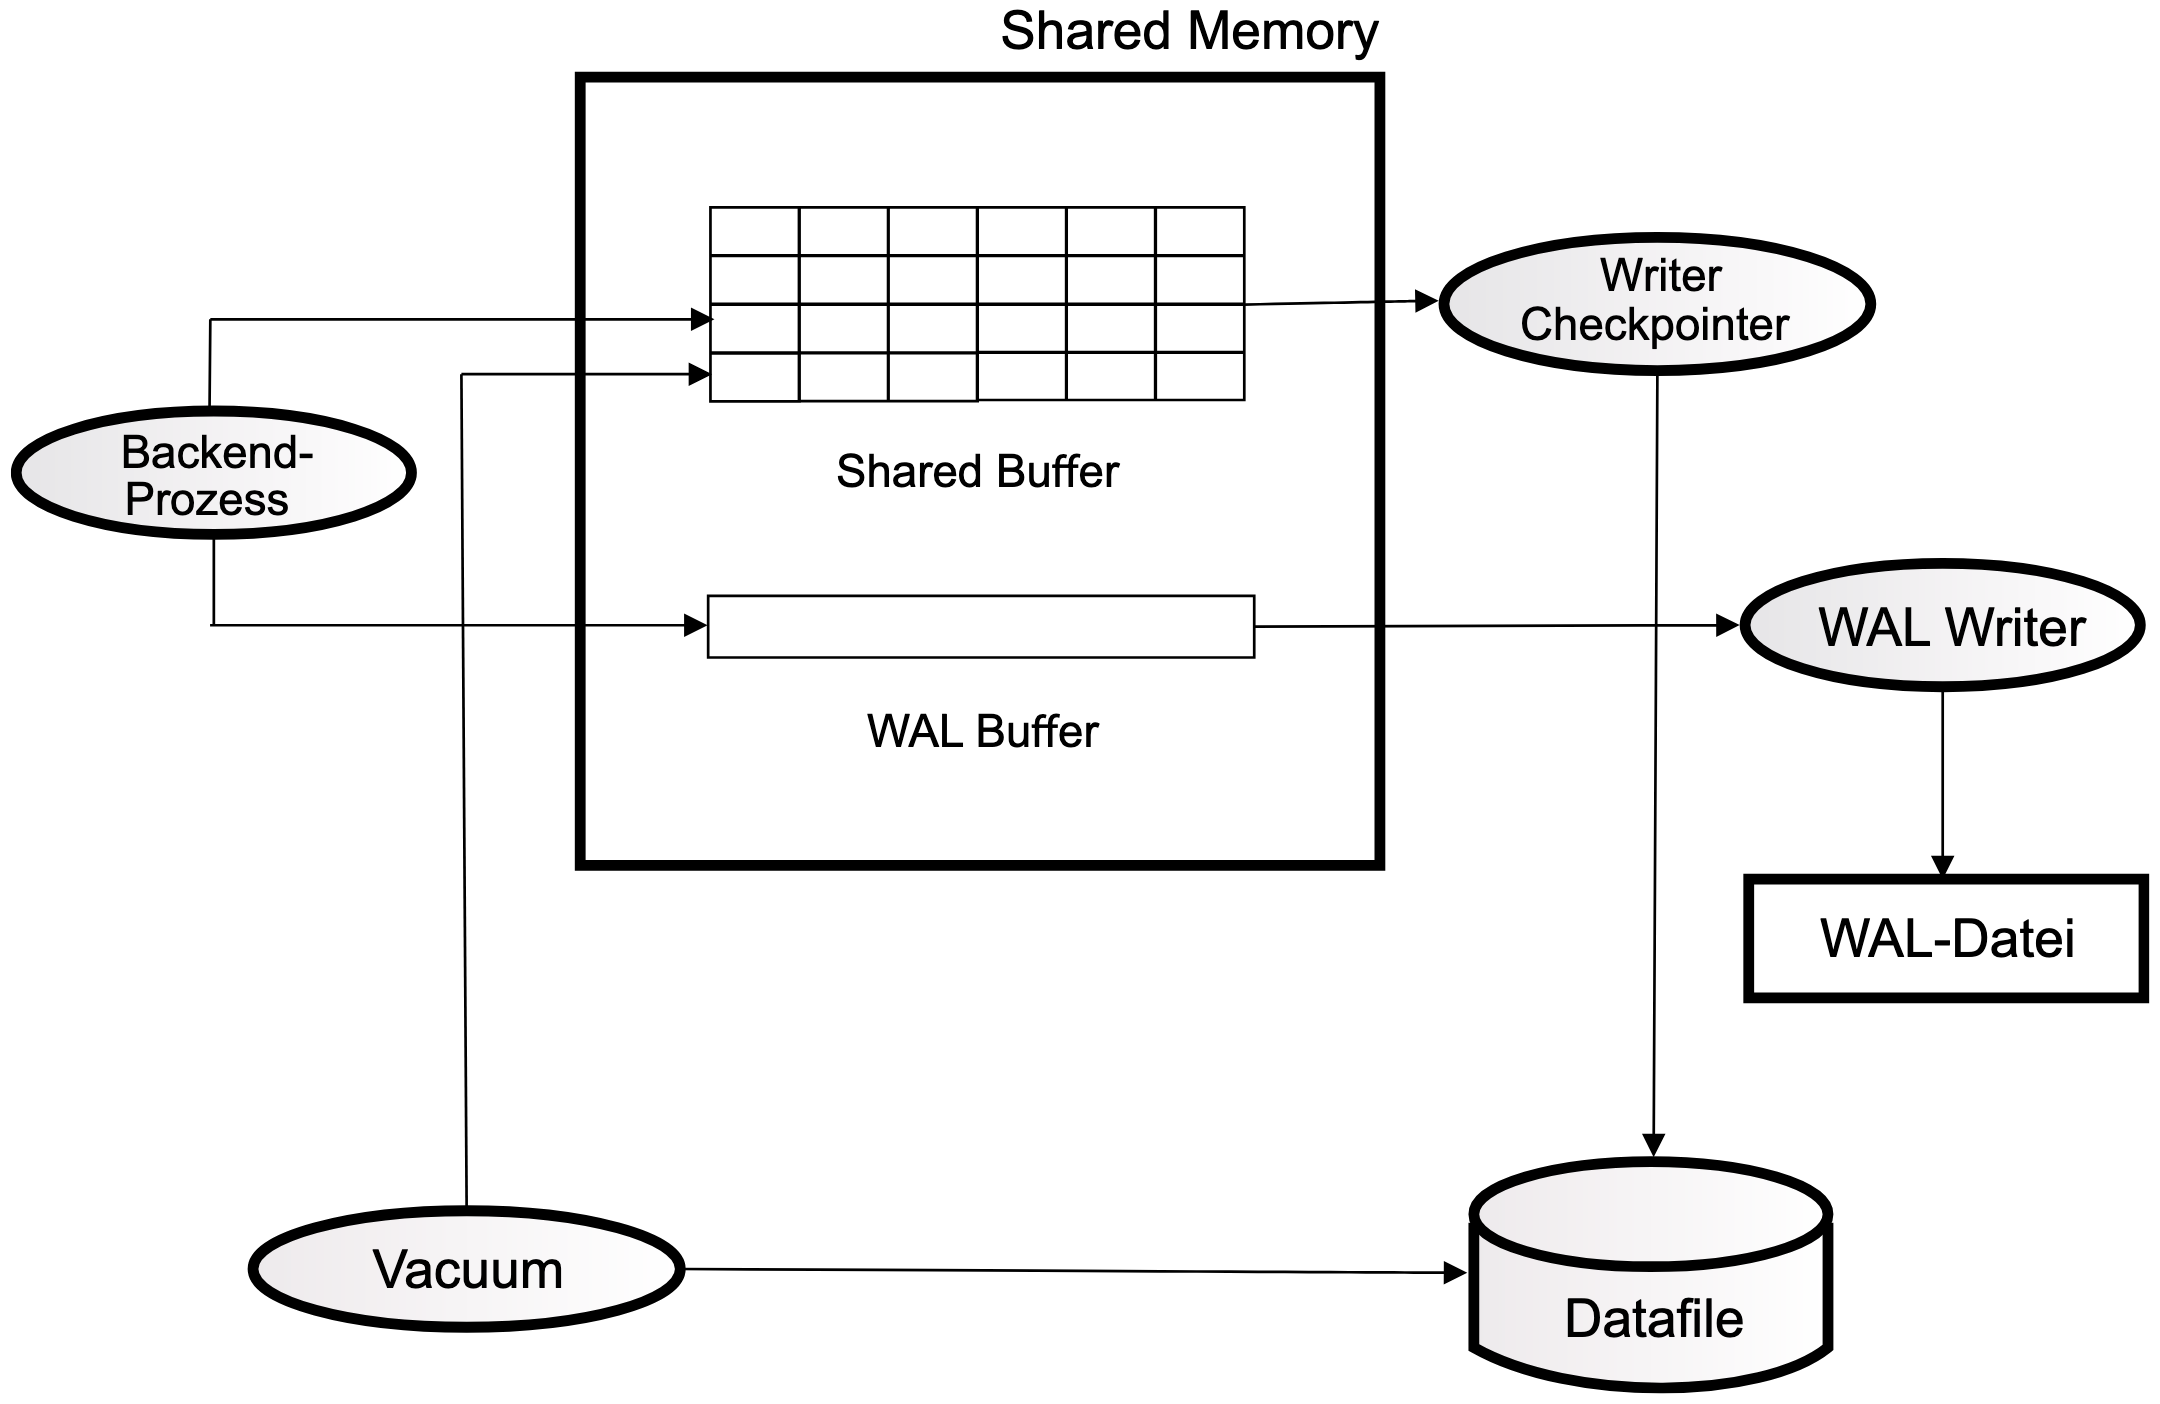
\includegraphics[width=\textwidth]{img/PostgreSQL Aufbau.png}
\caption{PostgreSQL Architektur. Quelle: \cite{Froehlich2022} S. 33 Bild 4.1}
\label{fig:Architektur}
\end{figure}

PostgreSQL besteht aus einer Kombination von Speicher und Prozessen. Bei Unix-Systemen sind diese Prozesse eigenständig, während sie bei Windows als Threads umgesetzt werden. Die wichtigsten Prozesse, die die Funktionalität von PostgreSQL abbilden, sind:
\begin{description}
    \item[Postmaster:] Der Hauptprozess, der die Verwaltung der anderen Prozesse übernimmt.
    \item[Checkpointer:] Dieser Prozess sorgt dafür, dass alle Änderungen in der Datenbank regelmäßig auf die Festplatte geschrieben werden.
    \item[Writer:] Verantwortlich für das Schreiben von geänderten Datenblöcken auf die Festplatte.
    \item[WAL Writer:] Handhabt das Schreiben von Transaktionsdaten in die Write-Ahead Log (WAL).
    \item[Autovacuum Launcher:] Dieser Prozess führt automatische Bereinigungen der Datenbank durch.
    \item[Archiver:] Archiviert die WAL-Dateien für eine verbesserte Rückverfolgbarkeit und Monitoring, besonders wichtig in produktiven Systemen.
    \item[Stats Collector:] Sammelt statistische Daten über die Nutzung von Sessions und Tabellen.
    \item[BGWorker:] Übernimmt verschiedene Hintergrundaufgaben.
\end{description}

\begin{figure}[h]
\centering
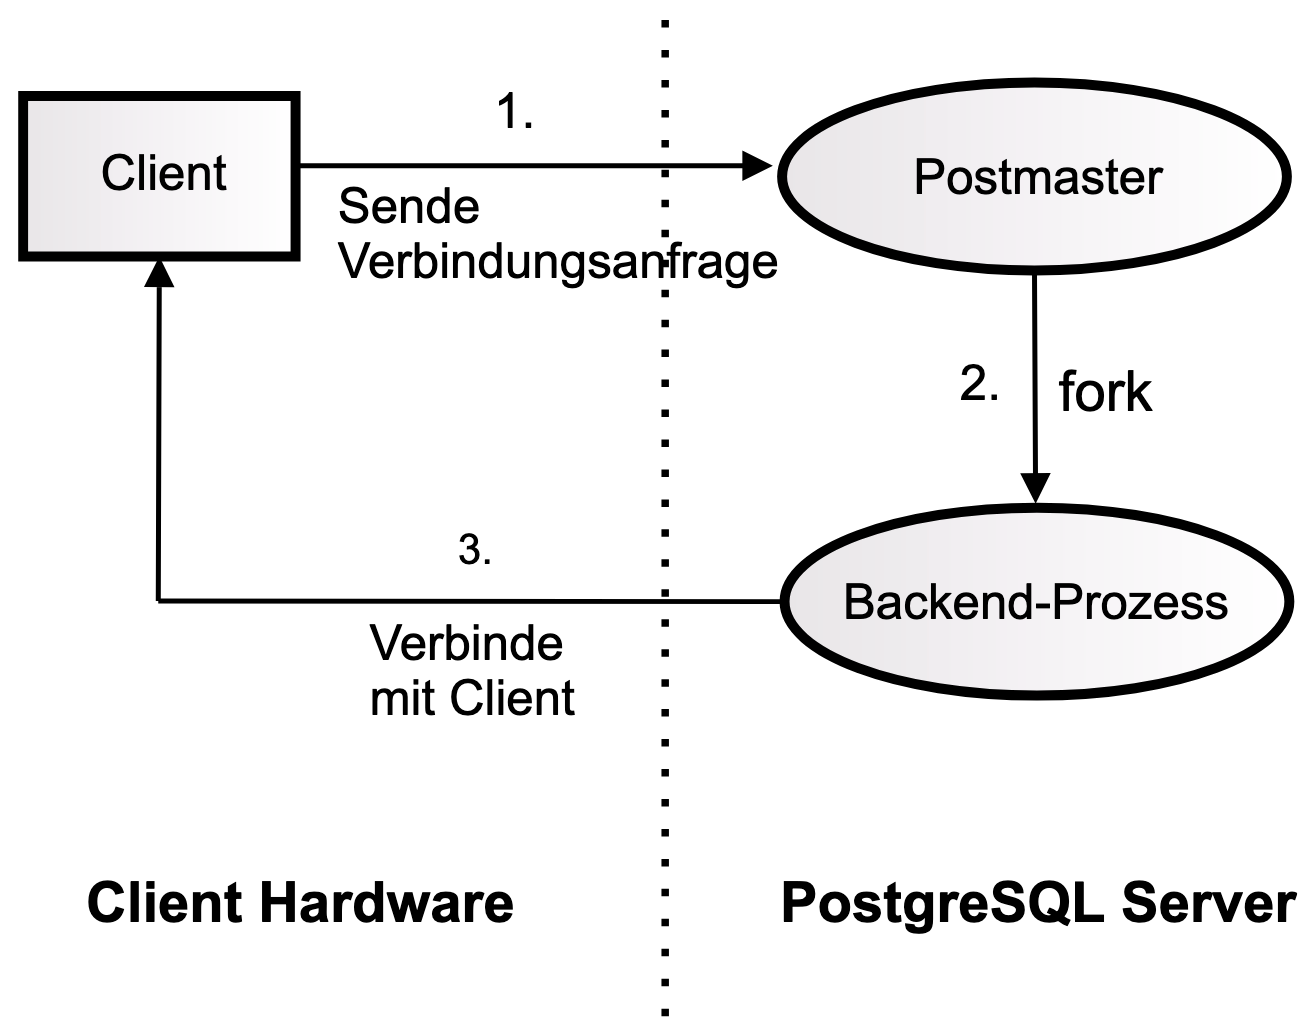
\includegraphics[width=\textwidth]{img/PostgreSQL Verbindungsaufbau.png}
\caption{Verbindungsaufbau von Client zum Server. Quelle: \cite{Froehlich2022} S. 35 Bild 4.3}
\label{fig:Verbindungsaufbau}
\end{figure}

Beim Aufbau einer Verbindung durch einen Client erstellt der Postmaster-Prozess nach erfolgreicher Authentifizierung und Autorisierung einen eigenen Backend-Thread. Die maximale Anzahl gleichzeitig aktiver Backend-Threads ist limitiert (Standard 100), was bedeutet, dass nach Erreichen dieser Grenze weitere Verbindungen abgelehnt werden.

\subsubsection{Speicherverwaltung und Performanceoptimierung}
Die Verwaltung von Speicher und die Optimierung der Zugriffszeiten auf Daten sind entscheidend für die Leistung von PostgreSQL. Da das Lesen von Daten von einer Festplatte vergleichsweise zeitaufwendig ist, setzt PostgreSQL auf verschiedene Mechanismen zur Verbesserung der Performance.

\begin{figure}[h]
\centering
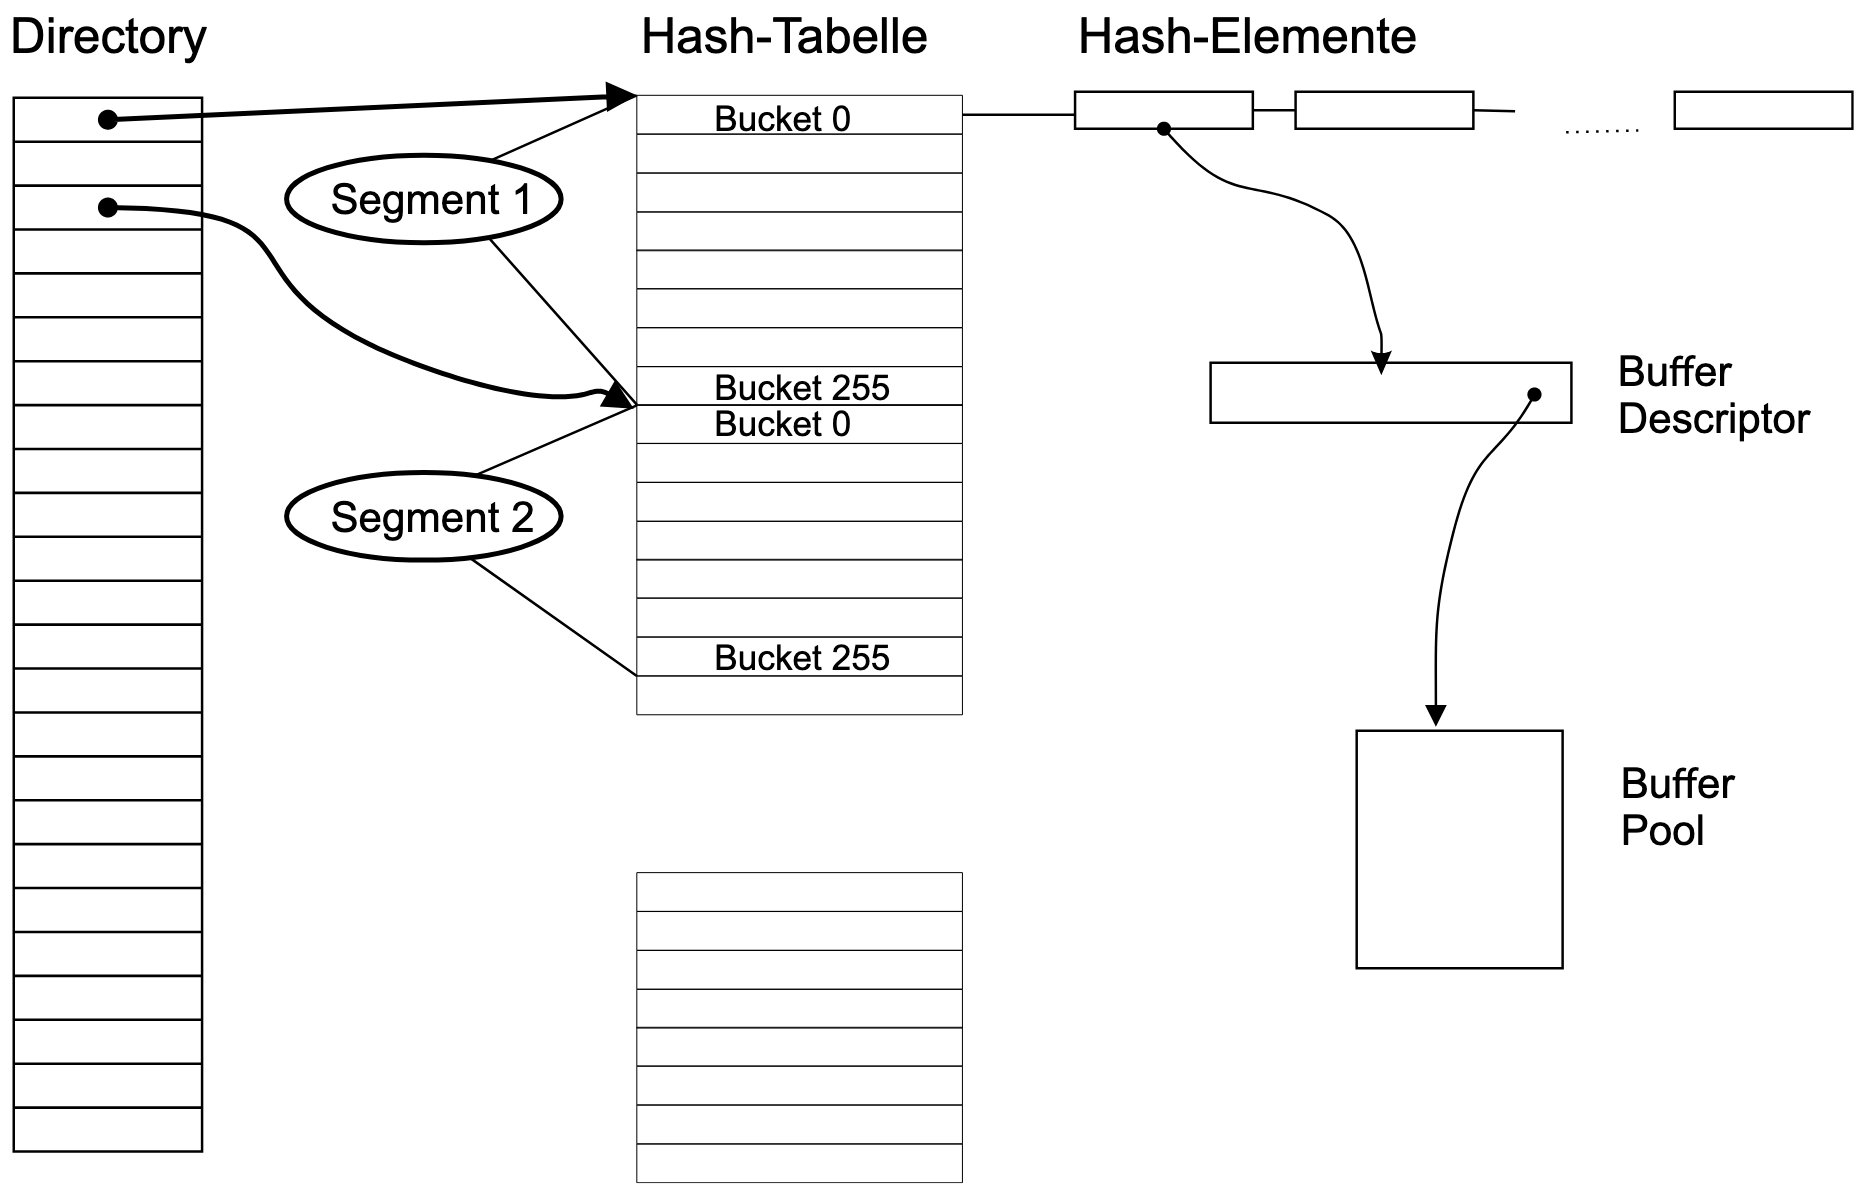
\includegraphics[width=\textwidth]{img/PostgreSQL Speciheraufbau.png}
\caption{PostgreSQL Speicherarchitektur. Quelle:  \cite{Froehlich2022} S. 37 Bild 4.4}
\label{fig:Speicheraufbau}
\end{figure}

\paragraph{Geteilter Speicher (Shared Buffer)}
Der Shared Buffer in PostgreSQL dient dazu, die Anzahl der Operationen auf der Festplatte zu reduzieren, indem er schnellen Speicher im RAM bereitstellt. Er besteht aus einer Hash-Tabelle, Hash-Elementen, einer Bufferbeschreibung und einer Buffersammlung. Die Hash-Tabelle ermöglicht ein schnelles Auffinden von Datensätzen, indem Hashwerte in Segmenten sortiert werden. Diese Segmente können sehr schnell durchsucht werden, da ihre Länge fest ist, was effiziente Speicherzugriffe ermöglicht.

Die Bufferbeschreibung enthält wichtige Steuerungsvariablen, wie z.B. den \code{\url{usage count}}, der die Relevanz eines Datensatzes im Speicher angibt. Der Speicherbereinigungsprozess (Eviction Process) durchsucht regelmäßig den Buffer nach irrelevanten Blöcken. Blöcke, die als irrelevant eingestuft werden, können überschrieben werden, sobald neuer Speicherplatz benötigt wird.

\paragraph{WAL Buffer und Checkpoints}
Der \ac{wal} Buffer ist darauf ausgelegt, Daten effizient auf die Festplatte zu schreiben. Dadurch müssen schreibende Prozesse nicht auf die tatsächliche Schreiboperation warten, sondern können die zu schreibenden Daten in den Buffer verlagern. Der \ac{wal} Buffer wird in regelmäßigen Intervallen (Standard 200 Millisekunden) überprüft und die Daten werden im Permanentspeicher gesichert, um die Ausfallsicherheit zu gewährleisten.

\code{Insert}-, \code{Update}- und \code{Delete}-Anweisungen werden über den \ac{wal}-Buffer verarbeitet. Diese Anweisungen werden in sogenannten \ac{wal}-Records gespeichert und sichern den Zustand der Daten auch bei einem Systemausfall. Ein Checkpoint, der den Speicherinhalt endgültig auf die Festplatte schreibt, wird unter bestimmten Bedingungen ausgeführt, wie etwa nach Ablauf eines festgelegten Intervalls, Erreichen einer bestimmten Buffergröße oder dem manuellen Auslösen eines Checkpoints.

\paragraph{Mehrere Datenblockversionen und Defragmentierung}

PostgreSQL unterstützt die gleichzeitige Bearbeitung von Datensätzen durch mehrere Sessions. Um sicherzustellen, dass sich die Sessions nicht gegenseitig beeinträchtigen, erhalten Datensätze eine Versionsnummer. Diese ermöglicht es, bei gleichzeitigen Abfragen und Bearbeitungen konsistente Daten bereitzustellen. Wenn eine Abfrage gestartet wird, kann anhand der Versionsnummer bestimmt werden, welcher Datensatz zum Zeitpunkt des Abfragestarts aktuell war.

Alte Datensätze, die nicht mehr benötigt werden, werden gelöscht, wodurch Lücken in der Tabelle entstehen. Diese Lücken werden durch den Autovacuum-Prozess freigegeben, sodass der Speicher für neue Datenblöcke verwendet werden kann. Bei Bedarf führt PostgreSQL ein \code{fullvacuum} durch, der die Tabelle vollständig defragmentiert, um Speicherplatz zurückzugewinnen und die Integrität der Versionsnummern zu gewährleisten.

\subsubsection{Permanentspeicherverwaltung}

Die Datenbanken von PostgreSQL werden im Verzeichnis \code{base} gespeichert, während der Tablespace in einem separaten Verzeichnis liegt. Tabellen und Indizes werden in Dateien von maximal einem Gigabyte Größe gespeichert; bei Überschreiten dieser Größe wird eine weitere Datei angelegt. Zusätzlich werden Dateien mit den Endungen \code{\_fsm} (Free Space Map) zur Adressierung des freien Speicherplatzes und \code{\_vm} (Visibility Map) zur Markierung von veralteten Datensätzen gepflegt.

Die Datenblocksammlung (Page) enthält Pointers auf die tatsächlichen Datenblöcke (Tuples). Jeder Datenblock wird durch eine Kombination aus der Datenblocksammlungsnummer und dem Offset des Pointers identifiziert. \cite{Froehlich2022}

\subsection{Exkurs: MongoDB}
MongoDB ist eine führende dokumentenorientierte NoSQL-Datenbank, die sich durch ihre Flexibilität und Skalierbarkeit auszeichnet. Sie wurde entwickelt, um einige der Einschränkungen traditioneller relationaler Datenbanken zu überwinden und bietet eine leistungsfähige Lösung für Anwendungen, die große Mengen an unstrukturierten oder semi-strukturierten Daten verarbeiten müssen. Im Gegensatz zu relationalen Datenbanken, die auf einem festen Schema basieren, erlaubt MongoDB ein dynamisches, schemaloses Datenmodell, das sich ideal für moderne, agile Entwicklungsprozesse eignet. In diesem Exkurs werden die Architektur und die technischen Merkmale von MongoDB detailliert beleuchtet, um deren Eignung für das \ac{nomtis}-Projekt zu bewerten.

\subsubsection{Speicherstruktur und Organisation}
MongoDB speichert Daten im \ac{bson}-Format, einem binären Format, das speziell für die Speicherung von Dokumenten mit \ac{json}-Syntax entwickelt wurde. \ac{bson} bietet eine effiziente Speicherung und Verarbeitung von Dokumenten, da es im Vergleich zu herkömmlichem \ac{json} kompakter und schneller zu verarbeiten ist. \ac{bson}-Dokumente können direkt in \ac{json} konvertiert werden, was die Integration mit Anwendungen erleichtert, die \ac{json} verwenden.

Die Speicherorganisation in MongoDB ist hierarchisch aufgebaut:
\begin{description}
    \item[Datenbank:] An der Spitze steht eine Datenbank, die mehrere Sammlungen (engl. Collections) enthalten kann.
    \item [Katalog:] Darunter befindet sich der Katalog, der Informationen über die Sammlungen und Indizes speichert.
    \item [Sammlung (engl. Collection)]: Eine Sammlung ist eine Gruppe von Dokumenten, die thematisch zusammengehören und ähnliche Strukturmerkmale aufweisen.
    \item [Dokument:] Auf der untersten Ebene steht das Dokument, das die eigentlichen Daten enthält.
\end{description}

\subsubsection{Katalog und Speicherverwaltung}

Der Katalog von MongoDB ist für die Verwaltung der Metadaten von Sammlungen und Indizes verantwortlich. Es gibt zwei Arten von Katalogen:
\begin{description}
    \item[Persistenter Katalog:] Dieser speichert Informationen dauerhaft auf der Festplatte und stellt sicher, dass Metadaten auch nach einem Neustart des Systems verfügbar bleiben. Der persistente Katalog wird in BSON-Dateien mit der Endung \code{\_mdb\_catalog} gespeichert und enthält Details über die Eigenschaften und Indizes der Sammlungen.
    \item [Memory-Katalog:] Der Memory-Katalog hält die Metadaten im RAM vor, um schnellen Zugriff zu gewährleisten und Ladezeiten zu minimieren. Operationen wie das Erstellen, Suchen, Iterieren und Schließen von Sammlungen werden im Memory-Katalog durchgeführt.
\end{description}

Um Dateninkonsistenzen zu vermeiden, wird der Memory-Katalog regelmäßig mit dem persistenten Katalog synchronisiert. Eine Versionsverwaltung stellt sicher, dass Änderungen korrekt nachvollzogen werden können, ohne dass es zu Lese-Schreib-Kollisionen kommt. MongoDB verwendet dabei das Copy-on-Write-Prinzip, bei dem nur dann eine Kopie des Datensatzes erstellt wird, wenn tatsächlich Änderungen vorgenommen werden. Dies minimiert den Speicherbedarf und erhöht die Effizienz.

\subsubsection{Speicherverwaltung und Defragmentierung}
Beim Löschen eines Eintrags in MongoDB erfolgt dieser Prozess in zwei Schritten:
\begin{enumerate}
    \item Löschen des Katalogeintrags: Zunächst wird der Eintrag sowohl im Memory-Katalog als auch im persistenten Katalog entfernt. Ein Verweis auf die Sammlung wird an den sogenannten \glqq Reaper\grqq{} übergeben, um sicherzustellen, dass keine neuen Zugriffe auf die Sammlung erfolgen, während aktive Lesezugriffe abgeschlossen werden.
    \item Endgültiges Löschen: Nachdem sichergestellt wurde, dass kein Rollback erfolgen kann, der die Daten der Sammlung wiederherstellen könnte, werden die Daten endgültig gelöscht.
\end{enumerate}

Freier Speicher, der durch das Löschen von Daten entsteht, wird in regelmäßigen Abständen für neue Datensätze freigegeben. Wenn der Speicher fragmentiert wird und viele kleine Lücken entstehen, führt MongoDB eine Defragmentierung durch. Dieser Prozess ordnet den Speicher neu an, kann jedoch Lese- und Schreiboperationen blockieren, was die Performance beeinträchtigen könnte. Daher sollte die Defragmentierung möglichst selten durchgeführt werden.

\subsubsection{Indizes und Abfragen}
Indizes in MongoDB werden hauptsächlich als B-Baum-Strukturen gespeichert, die eine effiziente Suche und Sortierung von Daten ermöglichen. Ein B-Baum-Index speichert die Daten strukturiert, ähnlich wie ein Dokument, und ermöglicht schnelle Zugriffe auf häufig abgefragte Felder. MongoDB erlaubt es auch, benutzerdefinierte Speicherstrukturen für Indizes zu erstellen, um spezifische Anwendungsanforderungen zu erfüllen. \cite{IamXander2024} \cite{themattman2024}

\subsubsection{BSON - Binary JSON}

\ac{bson} ist das zugrunde liegende Format für die Speicherung von Dokumenten in MongoDB. Es handelt sich dabei um ein binäres Format, das sogenannte Key-Value-Paare speichert und direkt in \ac{json} konvertiert werden kann. \ac{bson} ist jedoch deterministischer als \ac{json}, da es keine Flexibilität in der Darstellungsform bietet. Dies bedeutet, dass ein Datensatz in \ac{bson} immer in einer einzigen, festen Form dargestellt wird.

Ein \ac{bson}-Dokument beginnt immer mit einem 32-Bit-Ganzzahlwert, der die Länge des Dokuments angibt, und endet mit einem Null-Byte. Aufgrund dieser Struktur kann ein \ac{bson}-Dokument maximal ca. 2,147 Gigabyte an Daten umfassen. Die verschiedenen Datentypen, die \ac{bson} unterstützt, umfassen unter anderem:
\begin{description}
    \item[Int32 und Int64:] 4- bzw. 8-Byte lange Ganzzahlen.
    \item[Double:] 8-Byte lange Gleitkommazahlen nach dem IEEE 754-Standard.
    \item[Decimal128:] 16-Byte lange Gleitkommazahlen für hohe Präzision.
    \item[Array:] Ein Feld, das eine Liste von Werten speichert, wobei die Elemente wie Dokumente behandelt werden.
    \item[Null-Wert:] Ein spezieller Marker, der das Fehlen eines Wertes kennzeichnet.
    \item[Min- und Max-Schlüssel:] Marker, die den minimalen bzw. maximalen Wert eines Feldes darstellen.
\end{description}

Die strikte Struktur von \ac{bson} sorgt für eine konsistente und effiziente Speicherung und Verarbeitung von Dokumenten, was MongoDB zu einer leistungsfähigen Lösung für Anwendungen macht, die flexible und skalierbare Datenbanken benötigen. \cite{Velikhov}

\subsection{Diskurs: Vergleich von PostgreSQL und MongoDB für NOMTIS}
Die Auswahl der geeigneten Datenbanklösung ist ein zentraler Aspekt bei der Entwicklung von \ac{nomtis}. Da die internen Richtlinien PostgreSQL und MongoDB als verfügbare Optionen vorsehen, ist es entscheidend, die spezifischen Anforderungen von \ac{nomtis} zu analysieren und zu bestimmen, welche der beiden Datenbanken diese am besten erfüllt.

\subsubsection{Technische Anforderungen an NOMTIS}
\ac{nomtis} muss Benachrichtigungen effizient speichern, verwalten und flexibel verarbeiten können. Ein Hauptmerkmal von \ac{nomtis} ist die Fähigkeit, Benachrichtigungen mit potenziell komplexen und verschachtelten Datenstrukturen zu verwalten. Diese Datenstrukturen können variieren und sind oft nicht im Voraus vollständig definiert. Zudem sind eine hohe Zuverlässigkeit, Konsistenz und Skalierbarkeit erforderlich, um den Anforderungen eines modernen Benachrichtigungssystems gerecht zu werden.

\subsubsection{PostgreSQL: Technische Stärken und Grenzen}
PostgreSQL ist eine relationale Datenbank, die für ihre starke Unterstützung von \ac{acid}-Transaktionen, Datenintegrität und komplexen relationalen Abfragen bekannt ist. Diese Eigenschaften machen PostgreSQL ideal für Anwendungen, bei denen strenge Konsistenzanforderungen und komplexe Datenbeziehungen im Vordergrund stehen.

Die feste Struktur von PostgreSQL kann jedoch zu Einschränkungen führen, wenn es darum geht, dynamische und verschachtelte Datenstrukturen zu verwalten. Änderungen am Datenmodell erfordern eine Anpassung des Schemas, was in einem dynamischen Umfeld, wie es \ac{nomtis} erfordert, potenziell problematisch sein kann. Zudem ist PostgreSQL weniger effizient im Umgang mit tief verschachtelten oder unvorhersehbaren Datenstrukturen, was die Flexibilität des Systems einschränken könnte.

\subsubsection{MongoDB: Flexibilität und Skalierbarkeit}
MongoDB hingegen ist eine dokumentenorientierte NoSQL-Datenbank, die sich durch ihre schemalose Architektur und hohe Flexibilität auszeichnet. Die Speicherung erfolgt im BSON-Format, das eine effiziente Handhabung von \ac{json}-ähnlichen Dokumenten ermöglicht. Diese Struktur erlaubt es, Daten ohne festes Schema zu speichern, was für \ac{nomtis} von Vorteil ist, da die Benachrichtigungen beliebig komplexe und verschachtelte Daten enthalten können.

Ein weiterer zentraler Vorteil von MongoDB ist seine horizontale Skalierbarkeit. MongoDB unterstützt das sogenannte \glqq Sharding \grqq, bei dem Daten über mehrere Server verteilt werden, um eine hohe Verfügbarkeit und Performance sicherzustellen. Diese Fähigkeit zur horizontalen Skalierung ist besonders in einer Umgebung wie der \ac{sit} von Bedeutung, wo das Datenvolumen und die Anzahl der Nutzer kontinuierlich wachsen können.

Laut einer Untersuchung der MongoDB-Datenbank von Anjali Chauhan bietet MongoDB darüber hinaus eine hohe Leistung durch die Verwendung eingebetteter Datenmodelle, die E/A-Aktivitäten reduzieren, sowie durch Indizes, die schnellere Abfragen ermöglichen. \cite{Chauhan2019}
Diese Leistungsmerkmale machen MongoDB besonders geeignet für Anwendungen, die auf hohe Geschwindigkeit und effizienten Datenzugriff angewiesen sind.

\subsubsection{Schlussfolgerung: PostgreSQL als geeignete Wahl für Sensora}
Im Projekt Sensora ergibt sich aus den strukturellen Anforderungen und den funktionalen Zugriffsmustern ein klarer Bedarf an einem relationalen, transaktional konsistenten Datenbanksystem. Die Datenstruktur ist vordefiniert und weitgehend stabil. Pflanzen, Sensoren, Aktoren, Gruppen und Räume bilden klar abgegrenzte Entitäten mit definierten Beziehungen zueinander. Diese Relationen sind nicht nur logisch konzipiert, sondern stellen funktionale Notwendigkeiten dar – etwa wenn Sensoren bestimmten Pflanzen zugeordnet sind oder Aktionen nur innerhalb definierter Gruppenzugehörigkeiten zulässig sind.

Die Abfrageanforderungen im operativen Betrieb bestehen aus einer Mischung aus punktuellen Zugriffen (etwa auf aktuelle Sensorwerte oder Soll-Ist-Vergleiche) und zeitbasierten Auswertungen über große Datenmengen – insbesondere für die letzten 24 Stunden. Diese Anforderungen sind auf ein konsistentes, indexoptimiertes Schema angewiesen, das Joins effizient unterstützt und sich nicht durch Schema-Flexibilität, sondern durch strukturelle Integrität auszeichnet. Gleichzeitig ist paralleler Zugriff durch mehrere Microservices erforderlich, sodass Transaktionssicherheit und Isolation nicht nur erwünscht, sondern notwendig sind, um Inkonsistenzen bei konkurrierenden Schreiboperationen zu vermeiden.

PostgreSQL bietet genau für diese Art von Workload die passende Grundlage. Die stark normierten Strukturen des Sensora-Datenmodells profitieren von PostgreSQLs ausgefeilter Optimierung relationaler Abfragen, der zuverlässigen Durchsetzung referenzieller Integrität sowie der Möglichkeit, durch gezieltes Indexing auf Zeitstempel-Feldern hochfrequente historische Abfragen performant abzubilden. Selbst bei wachsendem Datenvolumen lassen sich durch Partitionierung oder die spätere Ergänzung durch TimescaleDB – ohne Verlassen der PostgreSQL-Basis – die Performanceanforderungen langfristig erfüllen, ohne strukturelle Kompromisse einzugehen.

Die fehlende Notwendigkeit für dynamische Schemas, polymorphe Dokumente oder eingebettete Strukturen eliminiert die Hauptargumente für ein dokumentenbasiertes System wie MongoDB. Vielmehr würde dessen Flexibilität in diesem Kontext eher potenzielle Inkonsistenzen begünstigen und zusätzliche Validierungslogik auf Anwendungsebene erforderlich machen – ein Mehraufwand, der durch das klar strukturierte Datenmodell nicht gerechtfertigt ist.

In Summe ist PostgreSQL damit nicht nur die technisch bessere Wahl, sondern die natürlichere Fortsetzung der bereits im Projektdesign angelegten Prinzipien: strukturierte, konsistente und integrierte Datenhaltung, auf die performant und sicher gleichzeitig von vielen Systemkomponenten zugegriffen werden kann.

  \section{Auswahl der Technologien f\"ur die entwickelten \\ Schnittstellen-Services}

Die im Rahmen des Projekts \textit{Sensora} entwickelten Schnittstellen-Services \"ubernehmen unterschiedliche Aufgaben innerhalb der Systemarchitektur, stellen jedoch alle zentrale Bausteine zur Kommunikations- und Steuerungsebene dar. Ihre Implementierung erfordert eine wohl\"uberlegte Auswahl geeigneter Technologien, die sowohl den funktionalen Anforderungen als auch den architekturellen, sicherheitstechnischen und betrieblichen Rahmenbedingungen gerecht werden.

In diesem Kapitel werden die getroffenen Technologieentscheidungen f\"ur jeden entwickelten Service einzeln erl\"autert, mit vergleichbaren Alternativen kontextualisiert und unter R\"uckbezug auf die definierten Anforderungen begr\"undet.

\subsection{Technologieauswahl f\"ur den Authentifizierungs- und Registrierungsdienst (Auth-Service)}

\subsubsection*{Zielsetzung und Kontext}

Der Auth-Service ist eine der sicherheitskritischsten Komponenten des Sensora-Systems. Er ist daf\"ur verantwortlich, neue IoT-Controller kontrolliert ins System aufzunehmen, ihnen eindeutige Kommunikationsidentit\"aten zuzuweisen und die Authentizit\"at dieser Ger\"ate eindeutig zu \"uberpr\"ufen. Zudem verwaltet er die Registrierung von Controllern in der zentralen Datenbank und erzeugt differenzierte Zugriffskan\"ale innerhalb der Messaging-Infrastruktur.

\subsubsection*{Verwendete Programmiersprache: Python}

F\"ur die Umsetzung des Auth-Service wurde die Programmiersprache \textbf{Python} gew\"ahlt. Python bietet eine sehr hohe Ausdrucksst\"arke bei gleichzeitig niedriger Komplexit\"at in der Syntax\cite{python_flask_prototyping}. Dies erlaubt eine fokussierte Umsetzung sicherheitskritischer Logik mit hoher Lesbarkeit und reduziertem Fehlerpotenzial. Die Sprache bietet native Unterst\"utzung f\"ur REST-APIs (via Flask), HMAC-Berechnungen (via \texttt{hashlib}) und JSON-Verarbeitung, was sie ideal f\"ur die Umsetzung des Auth-Service macht.

Im Vergleich zu Alternativen wie Java oder Go zeigt Python zwar leistungstechnische Schw\"achen bei hochfrequenten Systemen, bietet daf\"ur jedoch wesentlich h\"ohere Entwicklungsproduktiv\"itat \textendash{} ein entscheidender Vorteil im Rahmen eines begrenzten studentischen Projektzeitraums.

\paragraph*{Alternative Bewertung:}

Java bietet mit Spring Security zwar eine \"au\ss{}erst robuste Infrastruktur f\"ur Authentifizierungsmechanismen, ist jedoch deutlich komplexer im Deployment und ben\"otigt mehr Konfigurationsaufwand. Go bietet starke Performance und native Concurrency-Modelle, jedoch eine im Vergleich zu Python eingeschr\"ankte Bibliothekslandschaft f\"ur Security-Workflows. 

\paragraph*{Begr\"undung der Auswahl:}

Angesichts der Priorisierung von Entwicklungszeit, Lesbarkeit, Testbarkeit und Verf\"ugbarkeit passender Security-Tools wurde Python als die geeignetste Sprache f\"ur den Auth-Service identifiziert.

\subsubsection*{Authentifizierungsmechanismus: HMAC-basiertes Challenge-Response-Verfahren}

F\"ur die Authentifizierung der IoT-Ger\"ate wurde ein leichtgewichtiges Challenge-Response-Verfahren auf Basis von HMAC (Hash-based Message Authentication Code) implementiert. Diese Entscheidung basiert auf den Anforderungen an ein sicheres, serverseitig validierbares Verfahren ohne Notwendigkeit, Klartext-Zugangsdaten zu speichern oder zu \"ubertragen.

\paragraph*{Alternative Technologien:}
\begin{itemize}
  \item \textbf{OAuth 2.0:} Standard f\"ur Benutzer-Authentifizierung, jedoch komplex in der Implementierung f\"ur Maschinen-zu-Maschinen-Kommunikation.
  \item \textbf{JWT (JSON Web Token):} Geeignet f\"ur Token-basierte Sessions, jedoch problematisch hinsichtlich Zustandslosigkeit bei Ger\"aten mit hohem Sicherheitsanspruch.
  \item \textbf{Client-Zertifikate:} Sehr sicher, aber schwergewichtig in der Verwaltung f\"ur dynamisch zu registrierende IoT-Ger\"ate.
\end{itemize}

\paragraph*{Begr\"undung der Auswahl:}

Das HMAC-Verfahren erm\"oglicht die Validierung eines vorab generierten Ger\"ateschl\"ussels (Token), ohne diesen selbst senden zu m\"ussen. Durch serverseitige Generierung einer Challenge, die vom Ger\"at korrekt beantwortet werden muss, wird ein sicheres, manipulationsresistentes Protokoll etabliert, das gleichzeitig ressourcenschonend und einfach zu implementieren ist. Die Entscheidung orientiert sich damit an Best Practices f\"ur Ger\"ateauthentifizierung in Embedded-Umgebungen \cite{rfc2104_hmac}.

\subsubsection*{Kommunikationsmodell: REST-basierte API}

Der Service stellt seine Funktionalit\"at \"uber HTTP/REST-Endpunkte zur Verf\"ugung. Die Entscheidung f\"ur ein REST-Modell basiert auf der Notwendigkeit, den Dienst sowohl von Web-Frontends als auch von anderen Services (z.\,B. Mail-Service oder Solace-Konfiguration) ansprechbar zu machen.

\paragraph*{Alternative Technologien:}
\begin{itemize}
  \item \textbf{gRPC:} Hohe Effizienz, jedoch schwerer in Browser-Umgebungen integrierbar.
  \item \textbf{MQTT:} Bietet nur Publish/Subscribe, nicht geeignet f\"ur Request/Response-Workflows mit stateless APIs.
\end{itemize}

\paragraph*{Begr\"undung:}

REST bietet mit seiner stateless Architektur und breiten Toolunterst\"utzung (z.\,B. Swagger, Postman, curl) die optimale Basis f\"ur verteilte Systeme, insbesondere f\"ur administrative Operationen wie die Controller-Registrierung.

\subsubsection*{Interner Konfigurationsspeicher: JSON-Datei}

Die Informationen \"uber aktive Challenges und bereits registrierte Ger\"ate werden zus\"atzlich zur Datenbank in einer strukturierten JSON-Datei gespeichert. Dies erm\"oglicht schnelle Zugriffe auf tempor\"are Daten ohne Overhead einer persistierten Transaktion. Dieser pragmatische Kompromiss ist im Kontext studentischer Prototypen vertretbar.

\subsection{Technologieauswahl f\"ur den E-Mail-Verifikationsdienst (Mail-Service)}

\subsubsection*{Zielsetzung und Kontext}

Der Mail-Service stellt eine sicherheitsrelevante Verbindung zwischen Benutzerschnittstellen und Backend dar. Seine prim\"are Aufgabe ist die Versendung von E-Mail-\\Verifizierungslinks nach der Benutzerregistrierung. Damit fungiert er als zentrale Instanz zur initialen Verifikation von Benutzeridentit\"aten. Neben der Kommunikation mit einem SMTP-Server stellt der Dienst auch eine kontrollierte API zur Entgegennahme von Verifizierungsanfragen bereit.

\subsubsection*{Verwendete Programmiersprache: Python}

Die Entscheidung f\"ur Python basiert auf \"ahnlichen Argumenten wie beim Auth-Service. Python bietet durch Bibliotheken wie \texttt{smtplib} und \texttt{email.mime} einfache Schnittstellen zur Realisierung von SMTP-Kommunikation. Zus\"atzlich erlaubt die Verwendung von Flask eine unkomplizierte REST-Anbindung mit geringen Komplexit\"atsh\"urden. Im Rahmen des Projekts erm\"oglichte dies eine schnelle, wartbare und lesbare Implementierung des Dienstes.

\paragraph*{Vergleich mit Alternativen:}

Java (z.\,B. mit Spring Boot Mail) h\"atte eine robustere Infrastruktur geboten, w\"are jedoch mit erheblich h\"oherem Konfigurationsaufwand verbunden gewesen. Node.js wiederum bietet durch Pakete wie \texttt{nodemailer} eine gute Grundlage, ist jedoch im Team hinsichtlich Erfahrung weniger etabliert gewesen.

\paragraph*{Begr\"undung der Auswahl:}

Im Hinblick auf Entwicklungszeit, Lesbarkeit, Bibliotheksunterst\"utzung und Teamkompetenz wurde Python als pragmatische und effektive L\"osung gew\"ahlt.

\subsubsection*{E-Mail-Kommunikationsprotokoll: SMTP \"uber TLS}

F\"ur den Versand von Verifizierungsnachrichten wurde das Simple Mail Transfer Protocol (SMTP) in Kombination mit einer Transport Layer Security (TLS)-Verbindung eingesetzt. Diese Kombination bietet einen etablierten Standard f\"ur ausgehende Mail-Kommunikation mit Basisverschl\"usselung.\cite{smtp_tls}

\paragraph*{Alternativen:}

\begin{itemize}
  \item \textbf{REST-basierte Mailservices (z.\,B. SendGrid, Mailgun):} Bieten einfache APIs und statistische Auswertung, erfordern aber Drittanbieterkonten und externe Infrastruktur.
  \item \textbf{SMTP ohne Verschl\"usselung:} Unsicher und nicht datenschutzkonform.
\end{itemize}

\paragraph*{Begr\"undung:}

Die Entscheidung f\"ur SMTP \"uber TLS wurde getroffen, da ein Gmail für eine nicht zu Hohe Menge an Mails dies kostenlos ermöglicht und bereits zur Verf\"ugung stand und keine Drittanbieterintegration gew\"unscht war. Gleichzeitig konnten Sicherheitsanforderungen gewahrt bleiben.

\subsubsection*{Zugriffsschutz: Pre-Shared Key (PSK)}

Um zu verhindern, dass Dritte beliebige Verifizierungsanfragen senden, wurde der REST-Endpunkt des Mail-Service mit einem Pre-Shared Key abgesichert. Nur Systeme, die diesen kennen, k\"onnen autorisiert E-Mails ausl\"osen.

\paragraph*{Alternative Schutzmechanismen:}
\begin{itemize}
  \item \textbf{OAuth 2.0 oder API Tokens:} Sicher, aber unn\"otig komplex f\"ur einen geschlossenen Service.
  \item \textbf{Keine Authentifizierung:} Sicherheitsrisiko.
\end{itemize}

\paragraph*{Begr\"undung:}

Der Einsatz eines PSK ist ein einfacher, aber effektiver Schutzmechanismus, der in einem geschlossenen Systemumfeld wie Sensora praktikabel und ausreichend sicher ist.

\subsection{Technologieauswahl f\"ur den Datenpersistenzdienst (Database Writer)}

\subsubsection*{Zielsetzung und Kontext}

Der Database Writer nimmt eine zentrale Rolle in der persistenznahen Verarbeitung eingehender Sensordaten ein. Seine Hauptaufgabe besteht darin, kontinuierlich Datenpakete aus der Messaging-Infrastruktur entgegenzunehmen, diese auszuwerten und in strukturierter Form in das zugrunde liegende Datenbanksystem zu \"ubertragen. Eine besondere Herausforderung besteht dabei in der Notwendigkeit, sowohl hohe Verf\"ugbarkeit als auch Integrit\"at der Messdaten zu gew\"ahrleisten, selbst bei tempor\"aren Netzwerkproblemen oder inkonsistenten Eingangsnachrichten.

\subsubsection*{Programmiersprache: Python}

Die Implementierung des Database Writers erfolgte in Python. Die Entscheidung basiert auf der Kombination aus vorhandener Expertise im Projektteam, umfangreicher Bibliotheksunterstützung für JSON-Verarbeitung, Messaging-Systeme und Datenbankzugriffe sowie der leichten Wartbarkeit der Servicestruktur. In Python stehen mit Bibliotheken wie \texttt{paho-mqtt}\cite{python_mqtt}, \texttt{psycopg2} und \texttt{json} sofort einsatzfähige und stabile Werkzeuge für alle Teilaufgaben zur Verfügung.

\paragraph*{Vergleich mit Alternativen:}

Eine Implementierung in Go w\"are performant und speichereffizient, jedoch mit deutlich h\"oherem Aufwand bei der Bibliotheksintegration verbunden gewesen. Java h\"atte ebenfalls umfassende JDBC-basierte Anbindungen an relationale Datenbanken geboten, ist aber insbesondere f\"ur prototypische Implementierungen \"uberdimensioniert und aufw\"andig in Bezug auf Konfiguration und Deployment.

\paragraph*{Begr\"undung:}

Die Wahl von Python stellt einen optimalen Kompromiss zwischen Funktionalit\"at, Einfachheit und Flexibilit\"at dar. Dar\"uber hinaus konnte die gemeinsame Sprache mit den \"ubrigen Schnittstellen-Services genutzt werden, was die Homogenit\"at und Wartbarkeit der Gesamtplattform verbessert.

\subsubsection*{Messaging-Empfang: MQTT}

Der Database Writer konsumiert eingehende Nachrichten \"uber das MQTT-Protokoll, das vom zentralen Messaging-System vermittelt wird. MQTT wurde ausgew\"ahlt, da es mit seinem Publish/Subscribe-Paradigma und dem minimalen Protokoll-Overhead ideal auf intermittierende und latenzempfindliche Kommunikationsbeziehungen zwischen Sensoren und Auswertungssystemen zugeschnitten ist.\cite{mqtt_overview}

\paragraph*{Alternative Protokolle:}

\begin{itemize}
  \item \textbf{AMQP:} Industriestandard f\"ur Messaging, jedoch schwergewichtiger und nicht speziell f\"ur IoT optimiert.
  \item \textbf{HTTP Push:} Einfach zu implementieren, aber ungeeignet f\"ur kontinuierliche, bidirektionale Datenstr\"ome.
  \item \textbf{WebSockets:} Echtzeitf\"ahig, jedoch komplexer in der Integration mit klassischen Persistenzsystemen.
\end{itemize}

\paragraph*{Begr\"undung:}

MQTT bietet ein exzellentes Gleichgewicht zwischen Zuverl\"assigkeit, Ressourceneffizienz und Verbreitung im IoT-Bereich. Die Persistenzfunktionen des zugrunde liegenden Messaging-Brokers stellen zudem sicher, dass keine Daten durch kurzzeitige Netzwerkausf\"alle verloren gehen.

\subsubsection*{Fehlerbehandlung und Wiederholungsmechanismen}

Im Database Writer wurden explizite Retry-Mechanismen f\"ur die Datenbankanbindung integriert, um Datenverluste bei vor\"ubergehender Nichtverf\"ugbarkeit zu verhindern. Dies erfolgt \"uber ein warteschlangenbasiertes Zwischenspeichern nicht erfolgreicher Schreiboperationen, die periodisch erneut angesto\"ossen werden.

\paragraph*{Alternative Ans\"atze:}

\begin{itemize}
  \item \textbf{Fire-and-Forget-Ansatz:} Einfach, aber inakzeptabel bei Sicherheits- oder Zuverl\"assigkeitsanforderungen.
  \item \textbf{Transaktionsbasierte Protokolle:} W\"aren robuster, jedoch mit hohem Implementierungsaufwand verbunden.
\end{itemize}

\paragraph*{Begr\"undung:}

Die gew\"ahlte Methode stellt sicher, dass Datenverlust unter realistischen Bedingungen nahezu ausgeschlossen ist, ohne den Entwicklungsaufwand \"uber Geb\"uhr zu erh\"ohen. Die Wiederholungslogik kann bei Bedarf skalierbar erweitert werden.

\subsection{Technologieauswahl f\"ur die Zielwert-Schnittstelle (Setpoint API)}

\subsubsection*{Zielsetzung und Kontext}

Die Setpoint API erm\"oglicht die gezielte \"Ubertragung von Sollwerten an Steuercontroller, welche wiederum f\"ur die Regelung der Wasserzufuhr einzelner Pflanzen verantwortlich sind. Damit bildet sie eine Br\"ucke zwischen Benutzeranwendungen bzw. Systemkomponenten mit Steuerlogik und der dezentralen Aktorik des Systems. Die wesentliche Herausforderung besteht darin, eine flexible, zielgerichtete Kommunikation mit hoher Ausfallsicherheit und Ger\"atespezifit\"at zu gew\"ahrleisten.

\subsubsection*{Programmiersprache und Framework: Python mit Flask und Flasgger}

Die Implementierung erfolgte in Python, da bereits andere Systemkomponenten mit dieser Sprache realisiert wurden und eine hohe Wiederverwendbarkeit von Code sowie Konsistenz bei der Konfiguration gew\"ahrleistet werden sollte. Flask wurde als Web-Framework verwendet, da es eine schlanke Struktur mitbringt, sich hervorragend f\"ur RESTful-Services eignet und geringe Anforderungen an die Serverinfrastruktur stellt. Erg\"anzt wurde dies durch die Nutzung von Flasgger zur Generierung einer automatisierten Swagger-\\Dokumentation der REST-Endpunkte.\cite{flasgger_docs}

\paragraph*{Vergleich mit Alternativen:}

Alternativ w\"are FastAPI als modernere REST-Plattform denkbar gewesen, die native OpenAPI-Dokumentation, Validierung und asynchrone Verarbeitung unterst\"utzt. Allerdings wurde Flask aufgrund des stabileren Lern- und Erfahrungsstands im Team sowie vorhandener Funktionalit\"at bevorzugt.

\paragraph*{Begr\"undung:}

Die Kombination aus Flask und Flasgger erm\"oglichte eine wartbare und klar dokumentierte Schnittstelle mit kurzer Entwicklungszeit und einfacher Erweiterbarkeit. Die REST-Architektur passte gut zur Anforderung, kontrolliert und gezielt Steuerinformationen zu senden.

\subsubsection*{Kommunikationsmodell: Publish/Subscribe via MQTT \"uber Topics}

F\"ur die Weiterleitung der Sollwertnachrichten an den jeweiligen Controller wird das MQTT-Protokoll mit einer thematischen Strukturierung der Topics genutzt. Jeder Controller erh\"alt ein dediziertes Topic, dessen Aufbau die eindeutige Zuordnung der Nachricht erm\"oglicht. Dies entspricht dem Prinzip der Device-Adressierung in der IoT-Kommunikation.

\paragraph*{Vergleich mit Alternativen:}

\begin{itemize}
  \item \textbf{HTTP POST:} W\"are theoretisch f\"ur Push-Verhalten geeignet, erfordert jedoch persistente Adressen und erschwert dynamische Subscriptions.
  \item \textbf{AMQP:} Komplexer, mit mehr Overhead f\"ur das Szenario der gezielten Steuerung einzelner Endpunkte.
\end{itemize}

\paragraph*{Begr\"undung:}

MQTT erm\"oglicht eine sehr leichtgewichtige \"Ubermittlung mit der Option, persistente oder volatile Nachrichten zu senden. Die Topic-Struktur bietet eine flexible Adressierung ohne zus\"atzliche Verwaltungslogik. Die vorhandene Messaging-Infrastruktur mit Solace wurde konsequent weiterverwendet, was den Integrationsaufwand gering hielt.

\subsubsection*{Nachrichtenerstellung und Serialisierung}

Die Struktur der Sollwertnachricht wurde als JSON konzipiert, um sowohl Menschenlesbarkeit als auch Systemkompatibilit\"at zu sichern. Die Erstellung erfolgt mit Hilfe von Python-Bordmitteln, wodurch externe Abh\"angigkeiten minimiert werden konnten.

\paragraph*{Alternative Formate:}
\begin{itemize}
  \item \textbf{XML:} Etabliert, aber komplexer in der Verarbeitung.
  \item \textbf{Protobuf:} Effizient, aber f\"ur kleinere Projekte \"uberdimensioniert und weniger transparent.
\end{itemize}

\paragraph*{Begr\"undung:}

JSON bietet einen ausgezeichneten Kompromiss zwischen Standardisierung, Einfachheit und Interoperabilität. Es ist gut durch Firewalls und Broker-Systeme hindurch transportierbar und in praktisch jeder Sprache verarbeitbar.

\subsection{Technologieauswahl für den Initialisierungsskript-Dienst (Solace Init)}
\subsubsection*{Zielsetzung und Kontext}
Der Solace Init-Dienst wurde als automatisierter Initialisierungsmechanismus konzipiert, um beim Start des Systems die f\"ur die Kommunikationsarchitektur erforderlichen Messaging-Objekte auf dem Solace Broker anzulegen. Dabei handelt es sich insbesondere um Queues mit spezifischen Topic-Subscriptions, deren Struktur die Grundlage f\"ur das ger\"ateindividuelle Messaging im gesamten Sensora-System bildet. Ziel war es, eine einmalige, reproduzierbare und konfigurierbare Initialisierung ohne manuelle Eingriffe zu erm\"oglichen.

\subsubsection*{Begr\"undung der Broker-Wahl: Solace PubSub+ als Messaging-Plattform}
Die Wahl des Message Brokers stellt eine der zentralen Architekturentscheidungen im Sensora-Projekt dar. Die Anforderung bestand darin, ein performantes, fehlertolerantes und hochflexibles Messaging-System zu integrieren, das sowohl klassische Publish/Subscribe-Kommunikation als auch spezifische Anforderungen an Filterung, Persistenz und Authentifizierung erf\"ullt. Nach einem Vergleich mehrerer etablierter Systeme fiel die Entscheidung auf \textbf{Solace PubSub+}.\cite{solace_overview}

\paragraph*{Vergleich mit Alternativen:}

\begin{itemize}
  \item \textbf{Apache Kafka:} Hervorragend f\"ur Event-Streaming und hohe Datenvolumina, jedoch nicht nat\"urlich auf Topic-basiertes IoT-Publish/Subscribe ausgerichtet und ohne eingebaute Message Routing Features wie Topic Wildcards.\cite{mqtt_vs_kafka}
  \item \textbf{RabbitMQ:} Solide AMQP-Implementierung mit guter Dokumentation, jedoch schw\"acher in Bezug auf native MQTT-Unterst\"utzung, dynamische Topic-Strukturen und granulare Zugriffssteuerung auf Topics.
  \item \textbf{Mosquitto:} Leichtgewichtig und speziell auf MQTT ausgelegt, aber eingeschr\"ankt in Bezug auf Sicherheitsfeatures, Persistence-Mechanismen und Administration auf Enterprise-Niveau.
\end{itemize}

\paragraph*{St\"arken von Solace:}

Solace PubSub+ verbindet als Enterprise-Grade-Plattform mehrere Vorteile, die sich direkt aus den Anforderungen des Sensora-Projekts ergeben:

\begin{itemize}
  \item \textbf{Native Unterst\"utzung mehrerer Protokolle:} Solace unterst\"utzt MQTT, REST, AMQP und WebSockets nativ auf einem Broker. Damit konnten sowohl sensornahe Kommunikation \textit{(MQTT)} als auch service-interne Schnittstellen \textit{(REST)} integriert werden, ohne unterschiedliche Middleware-L\"osungen kombinieren zu m\"ussen.
  \item \textbf{Feingranulare Topic-Strukturen und Wildcards:} F\"ur die Adressierung einzelner Controller oder Sensortypen wurden hierarchische Topics mit Wildcard-\\Unterst\"utzung genutzt, wodurch sich flexible Abonnements realisieren lie\ss{}en.
  \item \textbf{Skalierbare Persistenzmechanismen:} Solace bietet sowohl volatile als auch persistente Delivery-Modes mit garantierter Zustellung, was f\"ur zeitkritische Steuerinformationen entscheidend ist.
  \item \textbf{Zentrale Administration via SEMPv2:} Die REST-basierte Konfigurationsschnittstelle (SEMPv2) erlaubt automatisierte, containerkompatible Initialisierungsskripte wie den hier beschriebenen Init-Service.
  \item \textbf{MQTT optimiert f\"ur IoT:} Die MQTT-Implementierung von Solace ist mit Fokus auf Latenzreduktion, Lastverteilung und Delivery-Garantien implementiert und eignet sich ideal f\"ur Embedded-Ger\"atekommunikation.
  \item \textbf{Security-Features:} ACL-Management, Authentifizierung auf Benutzer- und Topic-Ebene sowie TLS-Unterst\"utzung erm\"oglichen ein differenziertes Sicherheitskonzept.
\end{itemize}

\paragraph*{Zusammenfassende Begr\"undung:}

Solace PubSub+ wurde gew\"ahlt, da es in einzigartiger Weise hohe Anspr\"uche an Zuverl\"assigkeit, Integrationstiefe und Skalierbarkeit erf\"ullt. Die native Unterst\"utzung von MQTT ist f\"ur IoT-Anwendungen essenziell, w\"ahrend die gleichzeitige Verf\"ugbarkeit von Management- und Sicherheitsfunktionen auf Enterprise-Niveau den reibungslosen Betrieb in containerisierten Umgebungen sicherstellt. Dar\"uber hinaus empfiehlt auch der Hersteller Solace selbst den Einsatz von Python f\"ur schnelle Prototypenentwicklung im Bereich IoT \cite{solace_python_doc}.

\subsubsection*{Konfigurationsbasis: JSON-Datei}

Als zentrales Format f\"ur die Definition der zu erstellenden Queues und ihrer jeweiligen Subscriptions wurde eine strukturierte JSON-Datei verwendet. Dieses Format erlaubt eine deklarative Spezifikation der gesamten Messaging-Infrastruktur und kann sowohl von Menschen editiert als auch maschinell verarbeitet werden.\cite{json_best_practices}

\paragraph*{Vergleich mit Alternativen:}

\begin{itemize}
  \item \textbf{YAML:} Ebenfalls menschenlesbar, jedoch fehleranf\"alliger bei komplexeren Strukturen und nicht nativ durch alle Python-Standardbibliotheken unterst\"utzt.
  \item \textbf{XML:} Formal stark, aber syntaktisch schwergewichtig und in der Praxis f\"ur Konfigurationszwecke oft \"uberdimensioniert.
\end{itemize}

\paragraph*{Begr\"undung:}

JSON erf\"ullt im Kontext des Projekts das optimale Gleichgewicht zwischen Lesbarkeit, Standardisierung und Softwareunterst\"utzung. Es erm\"oglicht eine flexible Erweiterung der Initialisierungskonfiguration, z.\,B. durch Hinzuf\"ugen weiterer Queues oder komplexerer Subscription-Filter, ohne strukturelle Anpassungen am Code erforderlich zu machen.

\subsubsection*{Schnittstelle zur Messaging-Infrastruktur: Solace SEMPv2 API}

Die eigentliche Initialisierung erfolgt \"uber HTTP-Requests an die SEMPv2-API von Solace PubSub+, einer offiziellen Verwaltungs- und Konfigurationsschnittstelle des Brokers. Diese REST-basierte Schnittstelle erlaubt das Anlegen, Konfigurieren und Pr\"ufen von Messaging-Komponenten wie Queues, Topics und ACLs im laufenden Betrieb.

\paragraph*{Vergleich mit Alternativen:}

\begin{itemize}
  \item \textbf{Admin GUI:} Bedienerfreundlich, aber nicht automatisierbar und nicht reproduzierbar.
  \item \textbf{CLI-Tools (solacectl):} Eher f\"ur DevOps-Prozesse geeignet, jedoch aufwendiger in der Einbettung in einen containerisierten Microservice.
\end{itemize}

\paragraph*{Begr\"undung:}

Die REST-API von Solace war f\"ur den Projektkontext besonders geeignet, da sie eine serviceinterne und vollautomatische Ansteuerung erm\"oglichte. Die Authentifizierung konnte \"uber Umgebungsvariablen geregelt werden, die in Docker Compose konfiguriert wurden, sodass die Schnittstelle sowohl sicher als auch einfach nutzbar war. Zudem erm\"oglicht SEMPv2 die Definition granulare Subscription-Filter direkt beim Queue-Erstellen, was eine exakte Abbildung der Messaging-Logik erm\"oglicht.

\subsubsection*{Fehlertoleranz und Wiederanlauf}

Das Init-Skript enth\"alt einfache Mechanismen zur Wiederanlaufbarkeit. Existierende Queues werden nicht erneut erstellt, sondern \"ubersprungen oder aktualisiert. Fehler bei der Kommunikation mit dem Solace-Broker werden protokolliert, und das Skript kann bei Bedarf mehrfach ohne Seiteneffekte ausgef\"uhrt werden.

\paragraph*{Begr\"undung:}

Diese Idempotenz ist essenziell f\"ur automatisierte Umgebungen, etwa bei der Nutzung von Docker Compose oder CI/CD-Pipelines. Durch sie wird vermieden, dass der Initialisierungsprozess bei einem Neustart ungewollt Konfigurationsfehler verursacht oder bestehende Objekte zerst\"ort.

	\section{Mobile Kompilierung mit Capacitor}
\label{chap:capacitor}

Ein zentrales Ziel der entwickelten Anwendung ist ihre Nutzbarkeit nicht nur als Web-App, sondern auch als mobile Applikation auf Android-Geräten. Dies wird durch die Integration von Capacitor ermöglicht.

\subsection{Funktionsweise von Capacitor}
Capacitor fungiert als moderne Brückentechnologie zwischen Web-Technologien und nativer Funktionalität. Die Vue-Anwendung wird dabei in eine WebView eingebettet und über ein Plugin-System mit nativen Funktionen verbunden, was eine hybride Nutzung nativer Hardware-Ressourcen und Web-Technologien erlaubt \cite{Singh2021, Giordano2024}. Der Build-Prozess beginnt mit dem Erzeugen des Produktions-Builds der Vue-App mittels \texttt{vite build}. Anschließend wird mit dem Befehl \texttt{npx cap add android} ein natives Android-Projekt erstellt. Die WebAssets der Anwendung werden mit \texttt{npx cap sync} in das Android-Projektverzeichnis \texttt{android/app/src/main/assets} überführt. Danach kann die App entweder direkt in Android Studio geöffnet oder mit der Kommandozeile gestartet werden.

\subsection{Nutzung nativer APIs}
Capacitor stellt eine Reihe nativer APIs zur Verfügung, die aus der Vue-Anwendung heraus direkt verwendet werden können. Dazu zählen unter anderem der Zugriff auf die Kamera, auf das Dateisystem sowie UI-Funktionen wie StatusBar, SplashScreen und Toast-Benachrichtigungen \cite{Singh2021}. Diese APIs werden durch offizielle \texttt{@capacitor}-Plugins bereitgestellt und erlauben den Zugriff auf Systemfunktionen, ohne dass plattformspezifischer Code geschrieben werden muss.

\subsection{Besonderheiten und Herausforderungen}
Bei der Entwicklung für mobile Geräte ergeben sich mehrere technische Herausforderungen. So muss der Vue Router im sogenannten "History-Modus" betrieben werden, da es sonst zu Problemen mit Deep-Links unter Android kommen kann \cite{CapacitorDocs}. Bei falscher Konfiguration können Routen nicht korrekt aufgelöst werden, was 404-Fehler zur Folge hat. Zudem führt die Nutzung der Bildschirmtastatur auf Mobilgeräten dazu, dass Eingabefelder teilweise verdeckt werden. Dieses Verhalten muss durch gezielte Event-Behandlung oder gestalterische Workarounds ausgeglichen werden. Auch der Zugriff auf Systemfunktionen wie Kamera oder Medien setzt unter neueren Android-Versionen explizite Berechtigungsabfragen voraus, die sorgfältig umgesetzt werden müssen \cite{Singh2021}.

\subsection{Vor- und Nachteile der Verwendung von Capacitor}
Der Einsatz von Capacitor bringt sowohl Vorteile als auch Einschränkungen mit sich. Ein wesentlicher Vorteil besteht darin, dass die Anwendung weiterhin auf Web-Technologien basiert und somit eine einheitliche Codebasis für Web- und Mobile-Plattformen verwendet werden kann. Zudem unterstützt Capacitor Hot Reloading, was die Entwicklung und das Debugging deutlich beschleunigt \cite{Singh2021}. Die Anwendung kann darüber hinaus nicht nur als native App, sondern auch als Progressive Web App (PWA) bereitgestellt werden. Auf der anderen Seite ergeben sich durch die Nutzung der WebView geringere Performancewerte im Vergleich zu vollständig nativen Anwendungen \cite{Giordano2024}. Auch ist der Zugriff auf bestimmte Systemfunktionen eingeschränkt, und die Pflege des nativen Projekts setzt Kenntnisse in Android Studio und dem Android-Entwicklungsprozess voraus.

\subsection{Bewertung für das Projekt}
Für die im Rahmen dieser Arbeit entwickelte Anwendung stellt Capacitor eine sinnvolle und praktikable Lösung dar. Da die gesamte Logik auf Web-Komponenten basiert und der Bedarf an nativer Funktionalität auf wenige Aspekte wie Kameranutzung beschränkt ist, bietet Capacitor eine effiziente Möglichkeit, eine mobile Version mit minimalem Mehraufwand bereitzustellen. Die Integration in den Entwicklungsworkflow verläuft nahtlos, wodurch die mobile Erweiterung der smarten Bewässerungssteuerung sowohl benutzerfreundlich als auch wartbar bleibt.



	\section{Auswahl von Vue.js für die Implementierung}
\label{sec:auswahl-vue}

Im Rahmen der Entwicklung eines webbasierten Frontends für ein intelligentes Bewässerungssystem fiel die Wahl auf Vue.js. Die Entscheidung begründet sich auf mehreren Faktoren:

\subsection{Modularität und Komponentenstruktur}
Vue ermöglicht eine klare Trennung von Funktionalität, Darstellung und Stil durch das Single-File-Component-Modell. Dies unterstützt die Wiederverwendbarkeit und die Wartbarkeit in mittelgroßen Anwendungen wie der vorliegenden \cite{VueGuide2024}. Komponenten lassen sich dabei hierarchisch strukturieren, durch Props und Events miteinander verknüpfen und flexibel wiederverwenden. Die damit verbundene Modularität ist ein zentraler Vorteil im Vergleich zu klassischen Monolith-Strukturen.

\subsection{Reaktivität und Datenbindung}
Die Composition API in Vue 3 erlaubt die strukturierte Wiederverwendung von Logik und bietet eine feinere Kontrolle über Komponentenlebenszyklen. Die Reaktivierung ist deklarativ und effizient, was zu einer reduzierten Komplexität führt \cite{VueCompositionAPI2020}. Im Gegensatz zur eher komplexen Reaktivierung in Angular oder den teils manuell zu verwaltenden Hooks in React bietet Vue ein konsistentes Modell, das einfacher zu testen und zu debuggen ist \cite{VueReactivity2016}. Insbesondere die automatische DOM-Synchronisierung bei Zustandsänderungen verringert den Entwicklungsaufwand erheblich.

\subsection{Community, Dokumentation und Lernkurve}
Im Vergleich zu Angular bietet Vue eine flachere Lernkurve und ist dennoch umfangreicher als React in seiner Grundausstattung. Besonders für kleine bis mittelgroße Teams ohne dedizierte DevOps- oder Backend-Abteilungen eignet sich Vue durch seine einfache Integration und das konsistente "{O}kosystem \cite{Allotey2023}. Die offizielle Dokumentation von Vue gilt als eine der besten im Bereich der Webframeworks und trägt wesentlich zur schnellen Produktivität bei \cite{VueGuide2024}. Hinzu kommt ein aktives Community-Umfeld mit einer Vielzahl an Open-Source-Bibliotheken und Erweiterungen.

\subsection{Flexibilität, Integration und Zukunftssicherheit}
Ein weiterer Vorteil von Vue ist seine hohe Flexibilität im Hinblick auf Tooling und Integration. Vue-Projekte können leicht mit modernen Build-Tools wie Vite kombiniert werden, welches durch schnelle Entwicklungszyklen und modulare Hot-Reloading-Mechanismen eine effiziente Frontendentwicklung ermöglicht. Durch die strikte Trennung von View- und Logikschicht lässt sich Vue problemlos mit REST-APIs, GraphQL oder WebSockets kombinieren. Zudem wird Vue kontinuierlich weiterentwickelt: Die Long-Term-Support-Strategie sowie eine klare Roadmap sprechen für eine hohe technologische Zukunftssicherheit.

\subsection{Vergleich: Options API vs. Composition API in Vue.js}
Vue.js unterstützt zwei zentrale Paradigmen zur Strukturierung von Komponenten: die klassische Options API und die moderne Composition API. Beide Modelle ermöglichen die Definition von Zuständen, Methoden, Lebenszyklus-Hooks und Reaktivität innerhalb einer \ac{SFC}, unterscheiden sich jedoch fundamental im Aufbau und in der Ausdrucksstärke.

\paragraph{Options API}
Die Options API stellt das klassische und lange Zeit dominante Paradigma zur Definition von Komponenten in Vue.js dar. Ihr zentraler Vorteil liegt in der klar strukturierten Gliederung der Komponentenlogik nach spezifischen Optionen wie data, methods, computed, watch und Lebenszyklus-Hooks. Diese Trennung erleichtert insbesondere Einsteigerinnen und Einsteigern den Zugang zur komponentenbasierten Entwicklung, da die Zuständigkeiten der einzelnen Blöcke unmittelbar nachvollziehbar sind. Die durchgängige Unterstützung in der offiziellen Vue.js-Dokumentation sowie in zahlreichen Community-Plugins trägt zusätzlich zur Zugänglichkeit und zur breiten Akzeptanz dieses Modells bei. Auch historisch bedingt ist die Options API weiterhin vollständig kompatibel und wird aktiv gepflegt, was ihre Relevanz in bestehenden Projekten unterstreicht \cite{VueGuide2024}.

\newpage
\begin{lstlisting}[caption=Beispiel Options API]
export default {
	data() {
		return {
			counter: 0
		}
	},
	methods: {
		increment() {
			this.counter++
		}
	}
}
\end{lstlisting}

Den Vorteilen stehen jedoch mehrere signifikante Einschränkungen gegenüber. Insbesondere bei wachsender Komplexität einer Komponente stößt die Options API an strukturelle Grenzen. Da Zustände und zugehörige Methoden nach Typ gruppiert und nicht funktional zusammenhängend strukturiert werden, entsteht bei umfangreicher Logik schnell eine fragmentierte Darstellung. Diese Fragmentierung erschwert nicht nur die Lesbarkeit, sondern auch die Wartbarkeit und Wiederverwendbarkeit von Code – vor allem dann, wenn sich Logik über mehrere Komponenten hinweg wiederholt. Zudem leidet die Options API unter einer eingeschränkten Typsicherheit im Umgang mit TypeScript, da Kontextinformationen wie this nicht ohne Weiteres typensicher aufgelöst werden können. Dies kann zu Laufzeitfehlern führen und behindert die statische Analyse durch TypeScript-Compiler \cite{VueGuide2024}.

\paragraph{Composition API}
Die mit Vue 3 eingeführte Composition API bietet eine moderne und hochgradig modulare Alternative zur klassischen Options API. Sie zielt insbesondere auf eine bessere Wiederverwendbarkeit und thematische Gruppierung von Logik ab. Ein zentrales Merkmal ist, dass Zustände, Methoden und Nebenwirkungen innerhalb der \texttt{setup()}-Funktion definiert werden. Dadurch lassen sich zusammenhängende Funktionsblöcke logisch gruppieren und als sogenannte Composables wiederverwenden. Dies erhöht die Wartbarkeit bei wachsender Komponentenkomplexität erheblich \cite{CompositionAPIFAQ}.

Ein weiterer Fortschritt besteht in der Einführung des sogenannten \texttt{<script setup>}-Blocks, der in Vue 3 als syntaktischer Zucker (syntactic sugar) über der Composition API liegt. Im Gegensatz zur expliziten Verwendung von \texttt{setup()} in einem klassischen \texttt{<script>}-Block vereinfacht \texttt{<script setup>} die Struktur, reduziert Boilerplate-Code und macht die Komponenten deklarativer und kompakter. Dabei werden alle im \texttt{<script setup>} definierten Variablen automatisch im Template verfügbar gemacht, ohne dass ein \texttt{return} erforderlich ist \cite{ScriptSetup}.
\newpage
\begin{lstlisting}[caption=Beispiel für die Composition API mit \texttt{<script setup>},numbers=left,label=lst:scriptsetup,language=html]
	<script setup lang="ts"> 
		import { ref } from 'vue' 
		const counter = ref(0) 
		const increment = () => { counter.value++ } 
	</script>
	\end{lstlisting}

Hier wird ein reaktiver Zustand \texttt{counter} über die Funktion \texttt{ref()} erstellt, welcher automatisch mit dem DOM synchronisiert wird. Die Funktion \texttt{increment} verändert diesen Zustand und steht im Template zur Verfügung.

Die Vorteile dieses Ansatzes liegen auf der Hand: Logik ist gruppiert, leicht extrahierbar und testbar, insbesondere durch Composables. Darüber hinaus bietet die Composition API eine exzellente Typsicherheit, insbesondere im Zusammenspiel mit TypeScript \cite{VueCompositionAPI2020}.

Allerdings ergeben sich auch gewisse Herausforderungen. Für Neulinge kann der reduzierte strukturelle Rahmen der \texttt{setup()}-Funktion zunächst weniger Orientierung bieten als die Options API. Zudem besteht bei unstrukturierter Nutzung die Gefahr einer unübersichtlichen, flachen Anordnung vieler Logikelemente ohne klare Gruppierung, was die Lesbarkeit und Wartbarkeit negativ beeinflussen kann \cite{CompositionAPIFAQ}.

Während die Options API ihre Stärken in der Klarheit und dem geringeren Einstieg hat, bietet die Composition API insbesondere in Kombination mit \texttt{<script setup>}, eine moderne, typsichere und wiederverwendbare Struktur für Vue-Komponenten - insbesondere für mittlere bis große Anwendungen mit komplexer Zustandslogik \cite{CompositionAPIFAQ}.

\paragraph{Einordnung im Projektkontext}
In der vorliegenden Anwendung wurde bewusst die Composition API eingesetzt, da sie sich durch eine deklarative, modulare und testfreundliche Struktur auszeichnet. Besonders in Kombination mit Composables, wie etwa für API-Zugriffe oder Formularvalidierungen, ließ sich dadurch eine bessere Trennung von Logik und Darstellung erreichen. Die Integration mit dem State-Management-Tool Pinia ist ebenfalls eng an die Composition API gekoppelt, was die Konsistenz im Projekt stärkt.


\subsection{Einschränkungen und Gegenmaßnahmen}
Vue bringt zwar Einschränkungen hinsichtlich \ac{SEO} mit sich, insbesondere ohne \ac{SSR}. Diese lassen sich jedoch durch Techniken wie Prerendering oder den Einsatz von Frameworks wie Nuxt.js abmildern. Für komplexes State-Management stehen mit Pinia und Vuex leistungsfähige Bibliotheken zur Verfügung \cite{VueMastery2023}.

\bigskip
Insgesamt stellt Vue.js einen geeigneten Kompromiss zwischen Einfachheit, Leistung und Erweiterbarkeit dar und erweist sich als besonders geeignet für domänenspezifische Anwendungen mit moderater Komplexität. Die Balance zwischen Einstiegstauglichkeit und technischer Tiefe macht das Framework sowohl für Lernzwecke als auch für professionelle Webentwicklung attraktiv.


	\section{Einsatz von Tailwind CSS und Shadcn-Vue}

Moderne Webentwicklung nutzt zunehmend Utility-First-CSS-Frameworks wie Tailwind CSS und komponentenbasierte UI-Bibliotheken wie Shadcn-Vue zur effizienten Erstellung ansprechender Benutzeroberflächen. Diese Werkzeuge bieten im Kontext von Vue.js signifikante Vorteile hinsichtlich Geschwindigkeit, Wartbarkeit und Designkonsistenz \cite{TailwindCSS}, \cite{ShadcnVue2023}.

\subsection{Tailwind CSS: Utility-First-Ansatz}
Tailwind CSS ist ein Utility-First-CSS-Framework, das es Entwicklern erlaubt, direkt im HTML Code Styling zu betreiben, anstatt klassische CSS-Klassen zu definieren. Dies erleichtert die Wiederverwendbarkeit und reduziert übermäßige Stylesheet-Komplexität \cite{TailwindCSS}.

\paragraph{Vorteile:}
\begin{itemize}
	\item \textbf{Performance:} Tailwind eliminiert ungenutztes CSS im Produktionsbuild.
	\item \textbf{Responsives Design:} Vordefinierte Breakpoints erleichtern die Anpassung an verschiedene Bildschirmgrößen.
	\item \textbf{Designkonsistenz:} Einheitliche Farben, Abstände und Größen durch Konfiguration.
\end{itemize}

\paragraph{Integration in Vue.js}
Durch vordefinierte Klassen lässt sich Tailwind optimal in Vue-Komponenten einbetten. Der Code bleibt deklarativ und wartbar. Mit Tailwind können komplexe Layouts wie Grid-basierte Dashboards oder mobile Navigationsleisten ohne zusätzliche CSS-Dateien umgesetzt werden.

\subsection{Shadcn-Vue: Komponentenbibliothek f\"ur Vue 3}
Shadcn-Vue ist ein Community-getriebener Port der beliebten React-Bibliothek Shadcn/UI f\"ur Vue 3. Sie basiert auf Radix UI und Tailwind CSS, womit sie eine hohe Anpassbarkeit bei gleichzeitiger Konsistenz gew\"ahrleistet \cite{ShadcnVue2023}.

\paragraph{Modularer Aufbau}
Im Gegensatz zu anderen UI-Bibliotheken installiert Shadcn-Vue Komponenten selektiv. Dies f\"uhrt zu einer schlankeren Anwendung und erh\"oht die Kontrolle \"uber das Styling.

\paragraph{Beispiele aus dem Projekt}
Die Anwendung verwendet u.a. folgende Shadcn-Komponenten:
\begin{itemize}
	\item \texttt{Tabs}, \texttt{Cards}, \texttt{DropdownMenus} in der Pflanzen- und Sensordarstellung
	\item \texttt{Switches} und \texttt{Tooltips} in der Detailansicht und den Einstellungen
	\item \texttt{AlertDialogs} f\"ur Benutzerbest\"atigungsprozesse
\end{itemize}

\subsection{Kombination beider Technologien im Frontend-Projekt}
Tailwind CSS dient als stilistisches Fundament, w\"ahrend Shadcn-Vue darauf aufbaut und vorgefertigte interaktive Komponenten zur Verf\"ugung stellt. Das Ergebnis ist eine moderne, performante und barrierearme Benutzeroberfl\"ache, die sowohl f\"ur Desktop als auch f\"ur mobile Endger\"ate optimiert ist.

\paragraph{Fazit}
Die Kombination von Tailwind CSS und Shadcn-Vue stellt eine moderne und leistungsf\"ahige L\"osung f\"ur das Design von Vue.js-basierten Single-Page-Anwendungen dar. Sie reduziert Entwicklungsaufwand, erh\"oht die Designkonsistenz und verbessert die Nutzererfahrung signifikant \cite{Guimaraes2021}, \cite{TailwindCSS}.

	\section{Internationalisierung der Anwendung in Vue.js}
\label{sec:i18n}

Die Internationalisierung (i18n) ist ein zentrales Gestaltungsprinzip moderner Webanwendungen, das es erlaubt, Benutzeroberflächen an verschiedene Sprachen, Kulturräume und regionale Konventionen anzupassen. Sie leistet einen essenziellen Beitrag zur globalen Zugänglichkeit und Nutzerzufriedenheit, indem sie Inhalte sprachlich und kontextuell an die Erwartungen der NutzerInnen anpasst \cite{Stallmann2015}.

\subsection{Motivation und Bedeutung}
Internationale NutzerInnen erwarten digitale Produkte in ihrer Muttersprache und kulturell vertrauten Darstellung. Studien und Marktanalysen belegen, dass eine Lokalisierung von Inhalten die Nutzungsbereitschaft sowie die Conversion Rates deutlich erhöht. Zudem werden Missverständnisse vermieden, die sich aus abweichenden Symbolsystemen, Farbcodes oder Datums- und Zahlenformaten ergeben können \cite{Stallmann2015}.

Auch aus Sicht der Systemarchitektur trägt Internationalisierung zur Skalierbarkeit und Nachhaltigkeit digitaler Anwendungen bei. Internationale Standards wie Unicode und Locale-Formate ermöglichen eine konsistente Darstellung über verschiedene Plattformen hinweg. Die konsequente Trennung von Quellcode und Textressourcen gilt dabei als Best Practice \cite{vuei18nDocs2024}.

\subsection{Technologiewahl: vue-i18n}
Zur Umsetzung der sprachlichen und regionalen Anpassung wurde in der vorliegenden Vue.js-Anwendung das etablierte Plugin \texttt{vue-i18n} eingesetzt. Es ist der De-facto-Standard im Vue-\"Okosystem zur Internationalisierung und bietet eine modulare Integration für Komponenten, Routing und State Management \cite{vuei18nDocs2024}. Das Plugin erlaubt unter anderem:

\begin{itemize}
	\item Sprachumschaltung zur Laufzeit mit Reaktivität.
	\item Einbindung sprachspezifischer JSON-Ressourcen.
	\item Nutzung der \texttt{Intl}-API zur Formatierung von Datum, Uhrzeit und Zahlen.
	\item Unterstützung von Platzhaltern, Mehrzahlformen und dynamischen Textkomponenten \cite{Krukowski2024}.
\end{itemize}

\subsection{Fazit}
Die Nutzung von \texttt{vue-i18n} erwies sich im Projektkontext als leistungsfähig, flexibel und zukunftssicher. Durch die Verbindung mit nativen JavaScript-Standards (\texttt{Intl}) sowie die einfache Einbindung in die Vue-Komponentenarchitektur konnten sprachliche Anforderungen effizient umgesetzt werden. Die gewählte Lösung orientiert sich an etablierten Best Practices und stellt eine skalierbare Grundlage für weitere Internationalisierungsschritte dar.



	\section{State-Management mit Pinia und Persistenz}
\label{chap:pinia}

Ein zentraler Bestandteil moderner Frontend-Anwendungen ist das effiziente und wartbare Zustandsmanagement. Im Kontext der Webanwendung zur Steuerung eines smarten Bewässerungssystems kommt die State-Management-Bibliothek \texttt{Pinia} zum Einsatz. Dieser Abschnitt behandelt die Motivation, Konzeption und Persistierung des globalen Applikationszustands mittels Pinia in Vue.js.

\subsection{Einordnung von State Management in SPAs}

In Single Page Applications liegt die Verantwortung für das Daten- und UI-Management vollständig im Frontend. Daraus ergeben sich Anforderungen wie die zentrale Verwaltung globaler Zustände etwa für eingeloggte Benutzer oder verbundene Geräte, die Wiederverwendung von Daten über Komponenten hinweg, die Synchronisierung mit Backend-Endpunkten sowie die Notwendigkeit einer dauerhaften Speicherung über Seitenreloads hinaus. Pinia, als moderne und offizielle Ablösung von Vuex in der Vue-3-Welt, erfüllt diese Anforderungen durch seine modulare, typesichere und reaktive Struktur \cite{Vuex} \cite{Allotey2023}.



\subsection{Persistenz mit \texttt{pinia-plugin-persistedstate}}

Ein zentrales Merkmal der Anwendung ist die Fähigkeit, den Zustand auch bei einem Seitenreload zu bewahren. Dies wird mithilfe des Plugins \texttt{pinia-plugin-persistedstate} erreicht, das es ermöglicht, ausgewählte Stores automatisch im \texttt{localStorage} des Browsers zu speichern \cite{VueMastery2023}. Jeder Store konfiguriert explizit, ob und wie persistiert wird.



\subsection{Bewertung und Grenzen}

Im praktischen Einsatz zeigt Pinia deutliche Vorteile hinsichtlich Strukturierung und Wartbarkeit des Zustands. Die modulare Trennung erlaubt eine gute Übersicht und fördert die Wiederverwendbarkeit einzelner Logikkomponenten. Durch TypeScript wird zudem eine hohe Typsicherheit erzielt, was insbesondere in größeren Projekten die Fehleranfälligkeit reduziert. Auch das Debugging gestaltet sich dank der Integration in die Vue DevTools effizient. Die Persistenz erlaubt Offline-Szenarien und schützt vor ungewolltem Datenverlust. Eine Herausforderung besteht in der Handhabung verschachtelter Ressourcenbeziehungen. So referenziert eine Pflanze beispielsweise ihren Raum, dieser wiederum eine Gruppe. Dieses potenzielle Problem wird in der Anwendung durch gezielte Backendabfragen und das gezielte Laden zusammengehöriger Ressourcenstrukturen bei Bedarf entschärft.

\subsection*{Fazit}

Pinia mit Persistenz stellt ein robustes und wartbares State-Management für Vue-Frontends bereit. Es erfüllt die Anforderungen an Konsistenz, Wiederverwendbarkeit, Performanz und Sicherheit und bildet damit die solide Grundlage für ein reaktives und benutzerfreundliches Smart-Gardening-System.


	
	\newpage
	
	\chapter{Umsetzung}
	\section{Beschreibung des Datenbankaufbaus}
Die Datenbank des Systems Sensora ist im Schema sensora organisiert und verfolgt eine klar strukturierte, relationale Modellierung mit durchdachter Referentialität und Typisierung. Sie unterstützt die zentralen Funktionen des Systems wie Benutzerverwaltung, Gruppenzugehörigkeit, Raum- und Pflanzenzuordnung sowie Sensor- und Steuerdaten.
\newpage
\begin{figure}[H]
\centering
%  \includesvg[width=\linewidth, height=0.9\textheight, keepaspectratio,inkscapelatex=false]{img/Datenbank Diagramm.svg}
  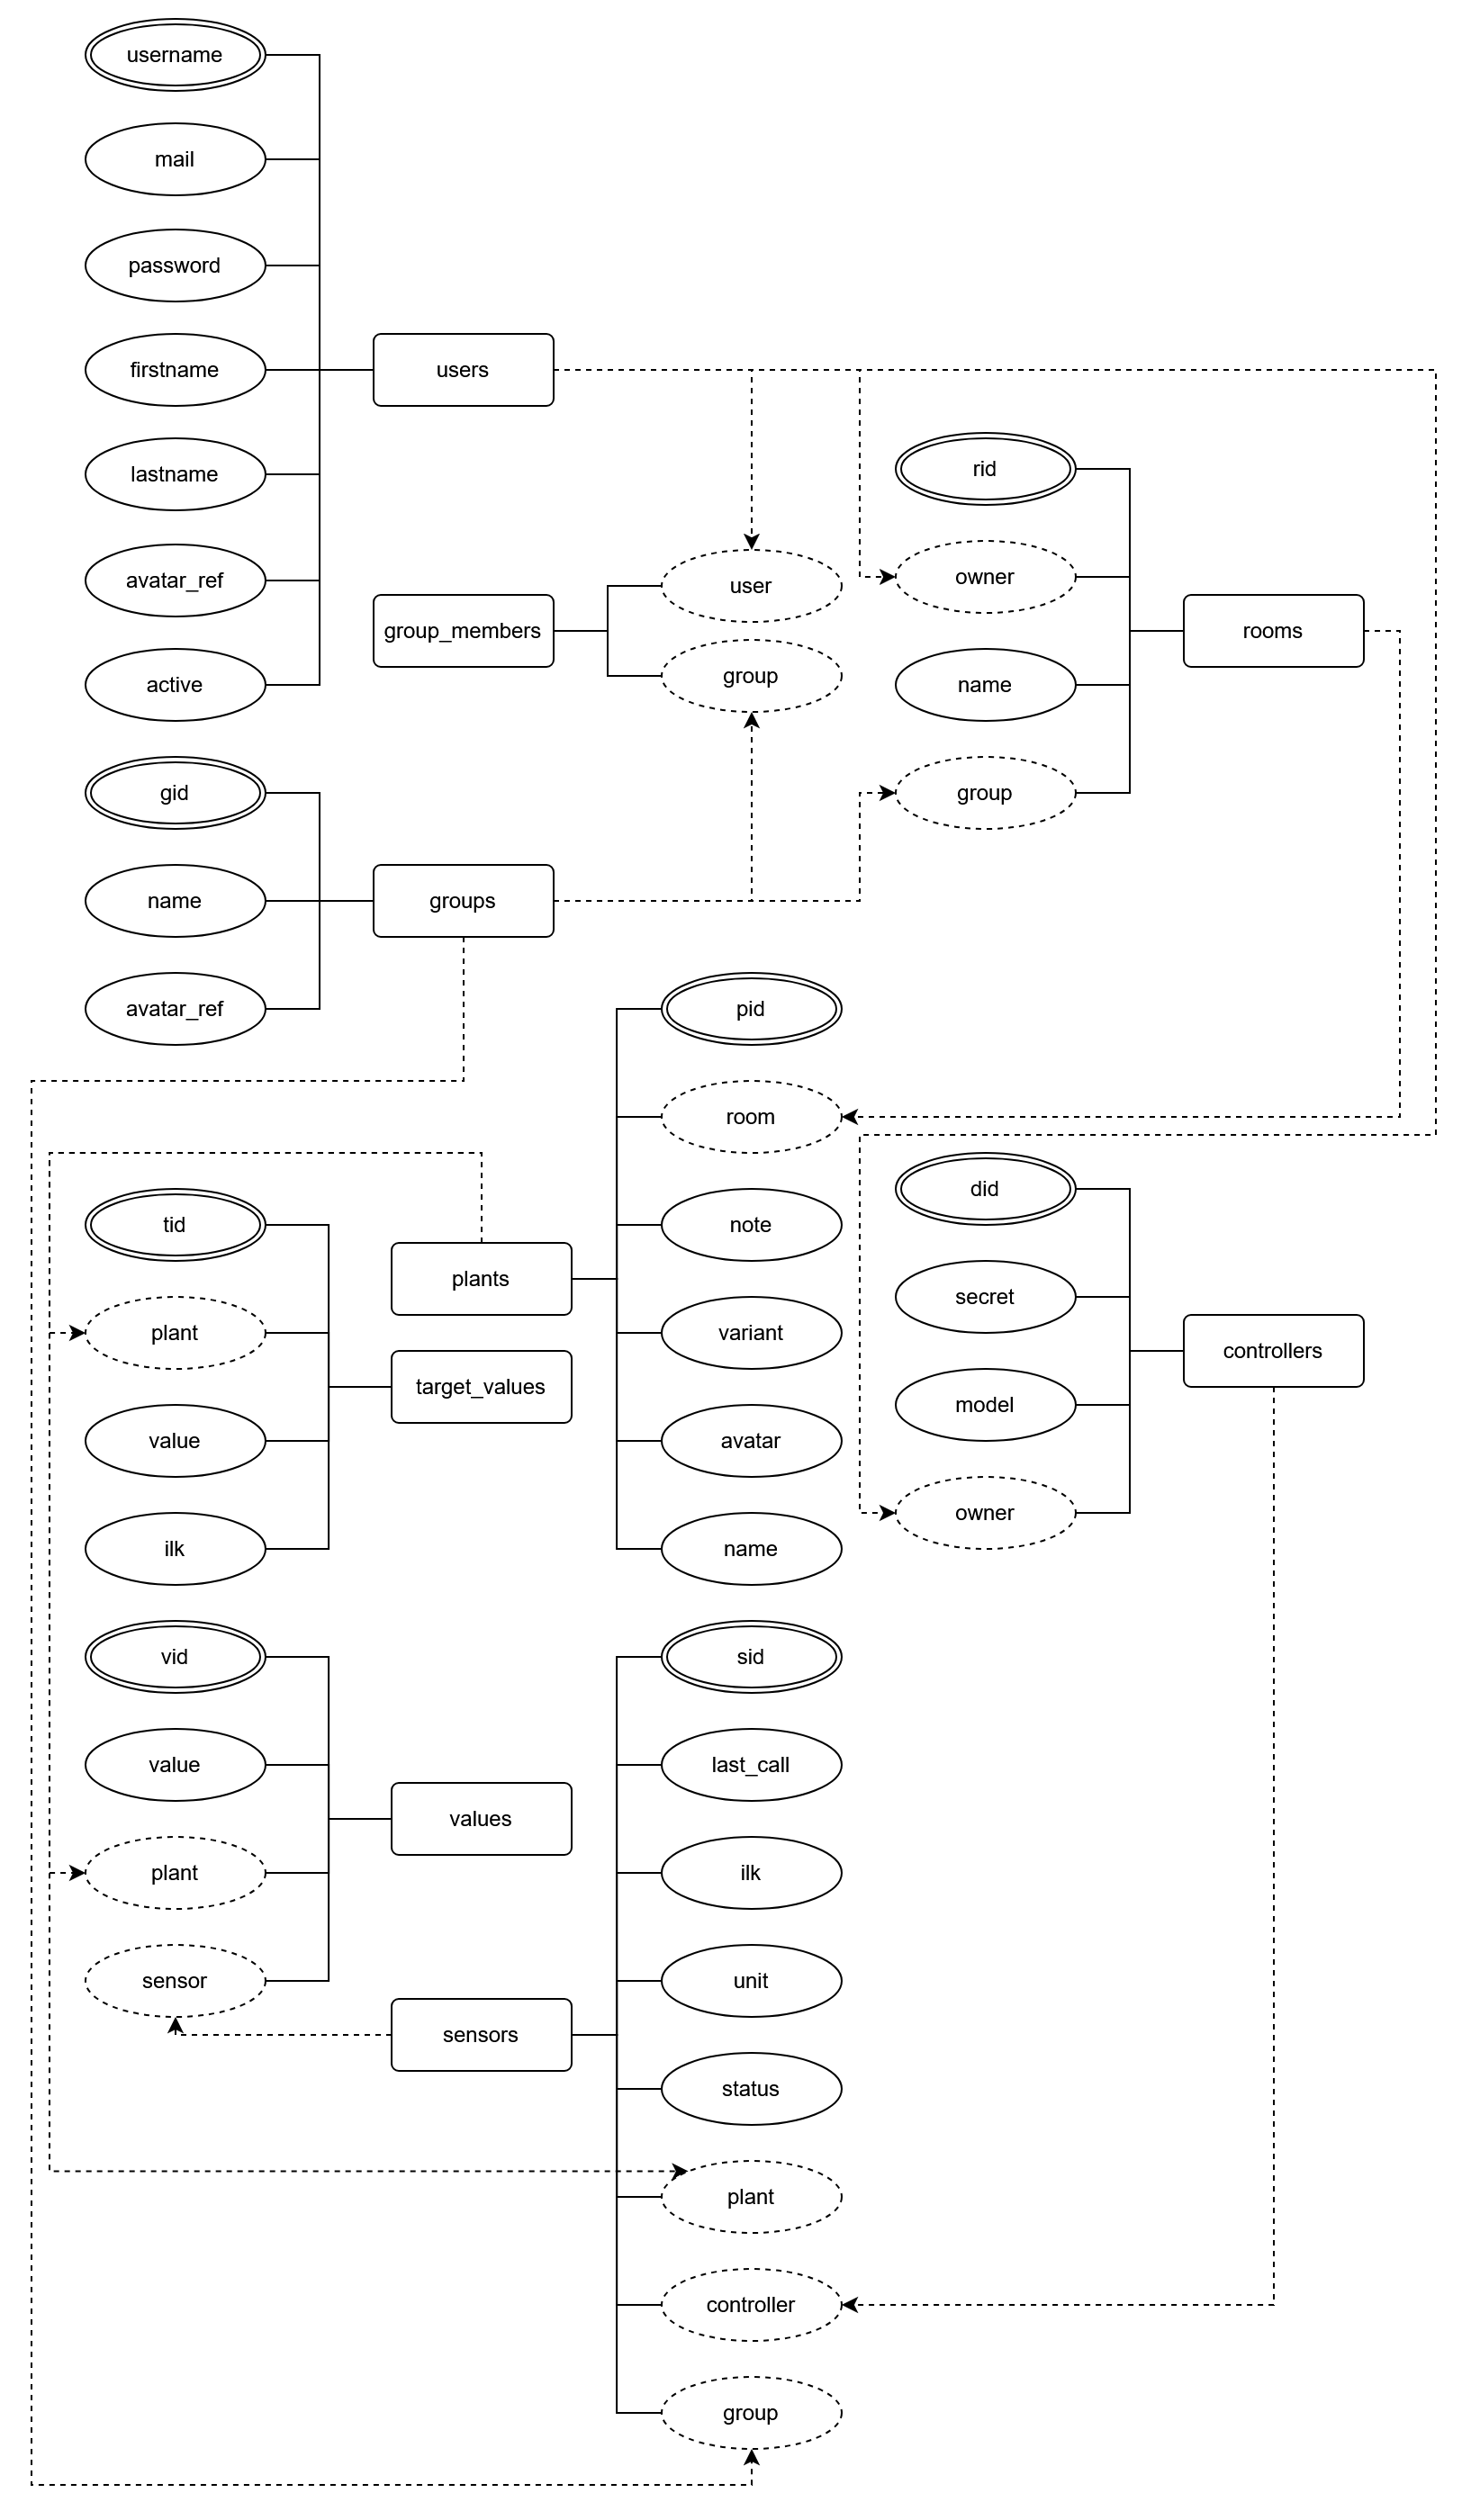
\includegraphics[width=\linewidth, height=0.9\textheight]{img/Datenbank Diagramm.png}
\caption{Sensora Datenbank Struktur}
\label{fig:sensora_datenbank}
\end{figure}
\newpage

\subsection{Struktur und Besonderheiten}
\begin{description}
    \item[Benutzerverwaltung:]
    Die Tabelle users bildet die zentrale Entität für Benutzer ab. Jeder Benutzer besitzt Pflichtangaben sowie einen referenzierten Avatar aus dem dedizierten ENUM-Typ sensora.avatar. Die E-Mail-Adresse ist eindeutig.
    \item[Gruppen \& Mitgliedschaften:]
    Gruppen (groups) können mehrere Mitglieder haben, realisiert durch die Join-Tabelle group\_members. Diese bildet eine klassische Many-to-Many-Beziehung zwischen Nutzern und Gruppen ab.
    \item[Räume \& Pflanzen:]
    Räume (rooms) können Gruppen zugeordnet sein und besitzen jeweils einen Eigentümer. Pflanzen (plants) sind immer einem Raum zugeordnet und dienen als Ankerpunkt für Messwerte.
    \item [Sensorik \& Steuerung:]
    Sensoren (sensors) sind mit Controllern (controllers) verknüpft und optional direkt mit einer Pflanze oder Gruppe verbunden. Jeder Sensor verwendet den ENUM-Typ sensora.status, um seinen Zustand zu klassifizieren.
    \item [Zielwerte \& Messdaten:]
    Pflanzen können über target\_values Zielgrößen definieren. Tatsächliche Messwerte werden in der Tabelle values gespeichert und jeweils einem Sensor sowie einer Pflanze zugeordnet.
\end{description}

\subsection{Technische Merkmale}
\begin{itemize}
    \item Es kommen ENUM-Typen zum Einsatz, um Felder wie Avatar und Status typensicher und standardisiert zu definieren.
    \item Sämtliche Fremdschlüsselbeziehungen nutzen CASCADE-Strategien zur Pflege von Konsistenz (z.B. beim Löschen von Benutzern oder Pflanzen).
    \item Indizes auf eindeutige Felder (z.B. mail, secret) erhöhen die Performanz gezielter Abfragen.
    \item Die Nutzung von Timestamps mit Standardwerten erlaubt eine automatische Protokollierung von Ereignissen wie Sensoraktivität.
\end{itemize}

Diese Datenbankstruktur ermöglicht eine flexible, erweiterbare und gleichzeitig robuste Grundlage für die Backend-Logik und garantiert eine nachvollziehbare Abbildung der fachlichen Entitäten.
  \section{Auth-Service: Geräteregistrierung und HMAC-Authentifizierung}
Der Auth-Service implementiert die sichere Registrierung und Anmeldung von Controllern mittels eines Challenge-Response-Verfahrens auf Basis eines vorab geteilten Geheimnisses (PSK). Dieser Dienst ist als Flask-Webanwendung realisiert und stellt HTTP-Routen für die Controller-Initialisierung, -Verifikation sowie eine Admin-Registrierung bereit. Er bildet damit das sicherheitskritische Bindeglied zwischen neuen Geräten und der Systeminfrastruktur: 
Geräte erhalten hier ihre individuellen Messaging-Zugangsdaten, sofern sie einen kryptographischen Besitznachweis erbringen. Im Folgenden werden die Architektur und der Ablauf des Auth-Service beschrieben, gefolgt von besonderen Implementierungsdetails wie der PSK-Überprüfung, Wiederanlaufbarkeit und der automatischen Broker-Konfiguration.
\subsection{Architektur und persistente Datenhaltung}
Der Auth-Service ist als Flask-Applikation mit dokumentierter REST-API (via Swagger/Flasgger) umgesetzt. Kern der Implementierung ist eine zentrale Konfigurationsdatei (auth\_config.json), die folgende Informationen persistent speichert:

\begin{enumerate}
    \item Authorized Controllers: eine Liste aller registrierten Controller mit deren Controller-ID (eindeutige Kennung), zugehörigem PSK (token) sowie einem Hash dieses Tokens (token\_hash). Zusätzlich werden Metadaten wie Modell, Besitzer (Benutzername) und Beschreibung gespeichert. Diese Datei dient als kleine lokale Datenbank, um bereits registrierte Geräte und ihre Geheimnisse nachzuhalten.
    \item Active Challenges: temporäre Herausforderungen (Challenges) im laufenden Authentifizierungsprozess.
    Für jeden angeforderten Auth-Vorgang wird ein zufälliger Challenge-String erzeugt und unter dem Schlüssel des token\_hash zwischengespeichert.
    Dies ermöglicht es, eingehende Antworten eindeutig der zuvor ausgegebenen Challenge zuzuordnen, selbst bei parallelen Anfragen.
    \item Solace Credentials: bereits für Controller erstellte Zugangs-Credentials für den Message Broker (Solace). Pro Gerät wird hier der erzeugte Broker-Benutzername und das Passwort abgelegt, um bei wiederholter Authentifizierung nicht erneut einen Broker-Account anlegen zu müssen.
\end{enumerate}
Die Konfigurationsdaten werden auf dem Container-Dateisystem unter /config/auth\_config.json verwaltet und durch Volume-Mounting persistent gehalten. Dadurch bleiben Registrierung und vergebene Credentials auch beim Neustart des Dienstes erhalten – ein wesentlicher Aspekt für Wiederanlaufbarkeit. Ergänzend hält der Auth-Service eine Datenbankverbindung (PostgreSQL via psycopg2) bereit, um neue Controller auch in der zentralen Systemdatenbank (sensora) zu registrieren. In der Tabelle sensora.controllers werden u.a. Device-ID, Modell, Besitzer und ein vom System generierter geheimer Schlüssel abgelegt. Letzterer unterscheidet sich vom PSK und dient ggf. anderen Zwecken (z.B. der Kommunikation mit externen Anwendungen), ohne das eigentliche PSK offenzulegen. Die doppelte Ablage (Datei und DB) der Registrierungsdaten mag auf den ersten Blick redundant erscheinen, ermöglicht jedoch sowohl schnelle lokale Zugriffe während des Auth-Handshakes als auch die Integration ins relationale Gesamtdatenmodell.

\subsection{Ablauf der Geräte-Registrierung und Authentifizierung}
Der Auth-Service bietet drei Haupt-Endpoints, die den Lebenszyklus eines Geräts abbilden: (a) Registrierung eines neuen Controllers (nur Admin), (b) Initialisierung des Authentifizierungs-Handshakes durch das Gerät und (c) Verifikation der Challenge-Response. 

Der Authentifizierungsablauf erfolgt in mehreren Schritten:
\begin{enumerate}
    \item Admin-Registrierung: Zunächst muss ein neuer Controller in das System aufgenommen werden. Ein Administrator (oder ein automatisierter Setup-Prozess) ruft dazu den Endpoint /api/admin/controller auf und übermittelt zumindest den gewünschten Besitzer (username) sowie optional eine vorgegebene Controller-ID und Modellbeschreibung. Der Request ist durch einen speziellen Admin-API-Key (Header X-Admin-Key) geschützt, sodass nur berechtigte Instanzen Geräte hinzufügen können. Bei Aufruf generiert der Service serverseitig ein zufälliges Token (PSK) für das Gerät (hier als UUID v4). Zusätzlich wird ein Token-Hash berechnet: mittels HMAC-SHA256 über das Token mit einem globalen Server-Geheimnis (TOKEN\_SECRET). Dieser Hash dient als öffentlicher Identifikator des Geräts, der das eigentliche Token nicht preisgibt. Anschließend werden die Gerätedaten in der auth\_config.json persistiert (authorized\_controllers) und ein Eintrag in der DB-Tabelle controllers erzeugt. Der Response an den Admin enthält Controller-ID, Token und Token-Hash, welche sicher an das Gerät für die Inbetriebnahme weitergegeben werden (z.B. manuell oder per Provisioning-App). Dieser einmalige Out-of-Band-Schritt stellt sicher, dass jedes Gerät ein individuelles geheimes Token besitzt, das dem Server bekannt ist.
    \item Challenge-Anforderung (Gerät → Auth-Service): Hat das Gerät vom Admin sein Token erhalten und wird erstmals online genommen, initiiert es den Authentifizierungsprozess über den Endpoint /api/controller/init. Dabei sendet das Gerät nur den Hash seines Tokens (token\_hash) im Request – das eigentliche Token bleibt geheim und wird nie direkt übertragen. Der Auth-Service prüft den Request und generiert eine kryptographisch zufällige Challenge (16 Byte Hex-String via secrets.token\_hex) als Antwort. Diese Challenge wird im Server-Konfigurationsspeicher unter active\_challenges zusammen mit einem Zeitstempel abgelegt, indiziert durch den token\_hash. Die Response an das Gerät enthält die Challenge als JSON. Aus Sicherheitsgründen findet an dieser Stelle noch keine Verifizierung statt – auch ein unbekannter Token-Hash erhält (vorläufig) eine Challenge. Der eigentliche Abgleich erfolgt erst im nächsten Schritt. Dieses zweistufige Verfahren erhöht die Sicherheit, da ein Angreifer ohne Besitz des PSK aus der Challenge alleine keinen Zugang erlangt. Wichtig ist, dass jede Challenge unvorhersehbar und einmalig ist, um Replay-Angriffe auszuschließen. Der Auth-Service stellt dies durch Verwendung eines Kryptografie-Moduls sicher (Python secrets \cite{pythonSecrets} bietet laut Dokumentation einen sicheren Zufallszahlengenerator für solche Token).
    \item Challenge-Response (Gerät → Auth-Service): Nach Erhalt der Challenge berechnet das Gerät die Antwort: Es verwendet sein geheimes Token und wendet darauf die gleiche Hash-Funktion an, die auch der Server kennt. Im Code wird dazu HMAC-SHA256 genutzt, wobei das Token als Schlüssel und der Challenge-String als Nachricht dient. Das Ergebnis ist die Challenge-Response (Hex-String). Diese Antwort schickt das Gerät zurück an den Auth-Service, zusammen mit seinem token\_hash (zur Identifikation der Challenge) und meist einem Benutzernamen oder Kontoinformationen des Eigentümers. Der Auth-Service schlägt nun in seiner Konfiguration den Eintrag zum token\_hash nach: Dort findet er das ursprünglich registrierte Token (PSK) und die zugehörige Controller-ID. Sollte kein Eintrag existieren, wird der Prozess abgebrochen – das Gerät war nie registriert oder der Hash unbekannt (Fehler 403). Andernfalls vergleicht der Server die vom Gerät gesendete HMAC-Antwort mit dem erwarteten Wert, den er selbst berechnet (hmac.compare\_digest() verhindert Timing-Angriffe bei der String-Bewertung). Stimmen Response und eigener Wert überein, ist bewiesen, dass das Gerät das geheime Token besitzt und somit authentisch ist. Dieses Challenge-Response-Verfahren stellt eine sichere Authentifizierung dar\cite{hmacRFC}, ohne das PSK selbst über das Netzwerk zu senden. Ein abgehörter Challenge/Response-Wert kann später nicht wiederverwendet werden, da bei der nächsten Anmeldung eine andere Challenge zum Einsatz kommt (kein statisches Passwort)
    \item Broker-Zugangsdaten erstellen: Nach erfolgreicher Verifizierung entfernt der Auth-Service die verwendete Challenge (Verbrauch der einmaligen Challenge) und fährt mit der Provisionierung des Geräts für das Messaging-System fort. Hier greift eine weitere wichtige Implementierungsentscheidung: Der Service konfiguriert den Solace-MQTT-Broker dynamisch über dessen Management-API (SEMP v2). Konkret wird geprüft, ob für den Controller bereits Broker-Zugangsdaten in solace\_credentials vorliegen. Ist dies der erste erfolgreiche Auth-Vorgang für dieses Gerät, generiert der Service mittels der Hilfsfunktion create\_solace\_user(controller\_id) einen dedizierten Broker-Account:
    \begin{enumerate}
        \item Es wird ein eindeutiger Client-Username für den Controller erstellt (z.B. controller\_ab12... gekürzt auf Basis der ID) und ein zufälliges Passwort (secrets.token\_urlsafe(32)).
        \item Für feingranulare Zugriffskontrolle richtet der Service ein eigenes ACL-Profil auf dem Broker ein. Dies geschieht über HTTP-Aufrufe an die SEMPv2-Konfigurationsschnittstelle des Solace-Brokers. Das ACL-Profil für den Controller erlaubt ausschließlich die für diesen Anwendungsfall nötigen Operationen:
        \begin{enumerate}
            \item Publish-Erlaubnis: Das Gerät darf nur auf seinem eigenen Topic-Pfad Messwerte publizieren. Im Prototoll wird das Topic-Muster sensora/v1/send/{controller\_id} verwendet. Über SEMP wird ein Topic Exception hinzugefügt, die genau dieses Topic für Publish freigibt (alle anderen werden per Default “disallow” gesetzt).
            \item Subscribe-Erlaubnis: Analog erhält das Gerät das Recht, Sollwert-Nachrichten zu abonnieren, die an sein spezifisches Target-Topic gesendet werden. Dies ist typischerweise sensora/v1/receive/{controller\_id}/targetValues. Auch hierfür wird programmgesteuert eine Ausnahme im ACL-Profil hinterlegt. Damit ist sichergestellt, dass der Controller nur Nachrichten empfängt, die explizit an ihn adressiert sind (und z.B. keine fremden Gerätedaten).
        \end{enumerate}
        \item Nachdem ACL-Profil und Berechtigungen erfolgreich angelegt wurden, erstellt der Service über die SEMP-API den Broker-Client-User und weist ihm dieses ACL-Profil zu. Sollte einer der Schritte fehlschlagen (z.B. aufgrund bereits existierender Einträge oder Verbindungsfehler zum Broker), bricht die Funktion ab und der Auth-Vorgang resultiert in einem Server-Fehler (HTTP 500). Im Erfolgsfall erhält der Auth-Service nun ein Credential-Paket bestehend aus Broker-URL, Username und Passwort für den neuen Controller.
    \end{enumerate}
    Die Nutzung der Solace Element Management Protocol API ermöglicht es, die Broker-Konfiguration zu automatisieren. Solace SEMP ist eine RESTful-Schnittstelle\cite{SolaceSEMP}, die das Anlegen von Objekten (Queues, Benutzer, ACLs etc.) per Skript erlaubt. Dadurch wird eine dynamische Inbetriebnahme neuer Geräte ohne manuelle Eingriffe möglich – ein wichtiger Vorteil im IoT-Kontext. Durch entsprechende Fehlerbehandlung (Auswerten des HTTP-Status: 200 Erfolg, 409 „Conflict“ bei bereits vorhandenen Ressourcen) ist die Funktion weitgehend wiederholbar, ohne Inkonsistenzen zu erzeugen. Beispielsweise würde ein erneuter Aufruf für denselben Controller erkennen, dass dessen Benutzerkonto schon existiert (der Auth-Service speichert dies ja auch in seiner config) und überspringt die Neuanlage. So bleibt der Prozess idempotent und ein Gerät könnte die Authentifizierung bei Bedarf erneut durchlaufen, um z.B. verlorene Credentials abzurufen.
    \item Registrierung abschließen und Antwort an Gerät: Zum Abschluss der /verify-Route führt der Auth-Service noch zwei Aktionen aus: (a) Eintrag in der Systemdatenbank: Falls noch nicht geschehen, wird der Controller endgültig in der sensora.controllers-Tabelle der DB vermerkt (inkl. Besitzverknüpfung zum Benutzerkonto, was zuvor im Request mitgesendet wurde). Außerdem kann hier optional ein Default-Sensor für den Controller in der DB angelegt werden (im Code wird bspw. ein Platzhalter-Sensor für Temperatur erstellt, um direkt Messwerte speichern zu können). (b) Secure Credential Delivery: Die vom Broker erzeugten Verbindungsdaten (Username/Passwort, Host) müssen nun dem Gerät mitgeteilt werden. Da diese Angaben sehr sensitiv sind, wurden besondere Maßnahmen getroffen, um sie vertraulich und integer zum Gerät zu übertragen. Der Server generiert zunächst einen einmaligen Session Key (eine randomisierte Byte-Sequenz mittels Fernet.generate\_key()), mit dem er die Credentials symmetrisch verschlüsselt (Fernet nutzt intern AES-128 in GCM-Modus\cite{fernetSpec} mit eingebauter HMAC für Integrität). Die so entstehende Ciphertext-Nutzlast wird als encrypted\_credentials bereitgestellt. Zusätzlich erzeugt der Server einen Credential-HMAC (credential\_key), indem er den Session Key mit dem ursprünglichen Geräte-PSK mittels HMAC-SHA256 signiert. Anschließend sendet der Auth-Service dem Gerät folgende Daten im JSON-Response:
    \begin{enumerate}
        \item session\_key: der im Base64-Format kodierte symmetrische Schlüssel,
        \item credential\_key: der HMAC (Hex-String) zur Absicherung,
        \item encrypted\_credentials: die verschlüsselten Broker-Zugangsdaten (Base64-Text).
    \end{enumerate}
    Diese Konstruktion erlaubt es dem Gerät, die erhaltenen Credentials auf Vertrauenswürdigkeit zu prüfen: Nur wenn es den gleichen HMAC über den Session Key mit seinem PSK berechnet und dieser mit dem credential\_key übereinstimmt, stammen die Daten eindeutig vom Auth-Service (der das PSK kennt). Damit ist ein Schutz gegen Man-in-the-Middle-Angriffe erreicht, selbst wenn kein vollwertiger TLS-Kanal vorhanden wäre – ein Angreifer könnte zwar den Session Key und Ciphertext stehlen, hätte aber ohne PSK keine Möglichkeit, gültige Daten vorzutäuschen. Nach erfolgreicher HMAC-Prüfung entschlüsselt das Gerät mit dem Session Key die Credentials und erhält so seinen persönlichen Broker-Login. Ab diesem Zeitpunkt kann sich der Controller am MQTT-Broker anmelden und regulär Sensordaten austauschen. Der einmalig verwendete Session Key ist nun obsolet.
\end{enumerate}
Abschließend bestätigt der Auth-Service dem Gerät die erfolgreiche Verifikation mit HTTP 200. Intern protokolliert er die erfolgreiche Authentifizierung und der Prozess ist abgeschlossen. Jegliche Fehlersituationen unterwegs (z.B. falscher Token, falsche Response, fehlende Eingabefelder) wurden mit aussagekräftigen HTTP-Codes (400 Bad Request, 403 Forbidden) und Log-Meldungen abgefangen, sodass das Gerät bzw. der Administrator direkt Rückmeldung über den Grund eines Scheiterns erhalten.


\section{Mail-Service: E-Mail-Verifikation von Benutzerkonten}
Der Mail-Service ist ein eigenständiger Webservice, der die Verifizierung von Benutzer-E-Mailadressen übernimmt. Im Gesamtsystem wird dieser Service genutzt, um nach einer Benutzerregistrierung sicherzustellen, dass die angegebene E-Mail dem Nutzer gehört und erreichbar ist – ein gängiges Verfahren, um Kontoaktivierungen durch den Nutzer selbst via Klick auf einen Bestätigungslink durchzuführen. Der Mail-Service wurde mit FastAPI (Python) umgesetzt, was die Erstellung asynchroner HTTP-Handler ermöglicht. Die Hauptaufgaben des Dienstes sind: Empfang der Verifikationsanfrage, Validierung mittels eines Pre-Shared Key (zur Absicherung interner Aufrufe), Generierung eines eindeutigen Bestätigungs-Tokens, Versand einer E-Mail mit Bestätigungslink via SMTP und abschließend die Verarbeitung des Bestätigungs-Clicks (Aktivierung des Kontos in der Datenbank).
\subsection{Architektur und Ablauf der E-Mail-Verifikation}
Der Mail-Service verfügt über zwei wesentliche Endpoints: einen POST-Endpoint /verify zum Anfordern einer Verifikationsmail und einen GET-Endpoint /confirm/{username}/{token} zum Bestätigen. Intern nutzt der Service eine PostgreSQL-Datenbankverbindung (asynchron via asyncpg), um Benutzerdatensätze zu prüfen und zu aktualisieren. Der Ablauf lässt sich wie folgt zusammenfassen:
\begin{enumerate}
    \item Anfrage zur Verifikation (POST /verify): Diese Schnittstelle wird vom übergeordneten System (z.B. dem Web-Frontend oder einem anderen Service) aufgerufen, sobald ein Benutzer eine Registrierung abgeschlossen hat oder eine E-Mail-Bestätigung angefordert wird. Der Request enthält typischerweise den Benutzernamen und die E-Mail-Adresse des Kontos. Zusätzlich erwartet der Service einen geheimen Schlüssel (key), der mitgeschickt wird. Dieser PSK (Mailservice) ist eine einfache Sicherungsmaßnahme, damit nur autorisierte Systeme (etwa das Frontend-Servermodul) den Versand von Verifizierungs-Mails auslösen können – damit wird verhindert, dass Unbefugte massenhaft Verifikations-E-Mails über die öffentliche API triggern. Der Service prüft also zuerst, ob der mitgesandte Schlüssel mit dem in den Umgebungsvariablen hinterlegten Wert (MAILSERVICE\_PSK) übereinstimmt. Ist dies nicht der Fall, wird mit HTTP 403 abgebrochen.
    Ist die Anfrage autorisiert, wird die angegebene Kombination aus username und mail in der Datenbank gesucht (SELECT * FROM sensora.users WHERE username=\%s AND mail=\%s). Nur wenn ein entsprechender Benutzeraccount existiert und noch als inaktiv markiert ist (dies wird indirekt geprüft, indem z.B. ein Feld active in der DB auf FALSE stehen sollte – im Code wird bei Nichtexistenz direkt 404 gemeldet), wird der Verifikationsprozess fortgesetzt. Im nächsten Schritt erzeugt der Service ein zufälliges Token als einmaligen Bestätigungscode. Hierzu wird Python secrets.token\_urlsafe(16) verwendet\cite{pythonSecrets}, was einen ~22 Zeichen langen kryptographisch sicheren String liefert. Das Token wird in einer in-memory Datenstruktur (tokens Dictionary) unter dem Schlüssel des Benutzernamens gespeichert. Anschließend wird ein Bestätigungslink erstellt, der die URL des Confirmation-Endpoints enthält (inkl. Pfadparameter für Username und Token). Dieser Link hat z.B. die Form: https://meinserver/confirm/alice/AbCdEfGh... – er enthält also das geheime Token.
    Nun versendet der Mail-Service eine E-Mail an die Adresse des Nutzers. Dafür wird ein SMTP-Server (hier Gmail SMTP auf Port 587) verwendet. Über Pythons smtplibwird eine TLS-geschützte Verbindung aufgebaut, der Mailaccount authentifiziert (SMTP-User und Passwort liegen in den Settings) und dann eine Textnachricht verschickt. Der E-Mail-Inhalt besteht aus einem kurzen Text mit der Aufforderung, den Link anzuklicken, um die Registrierung abzuschließen. Absender und Betreff sind entsprechend gesetzt (z.B. "Bitte bestätige deine E-Mail"). Nach erfolgreichem Versand gibt der/verify-Endpoint eine Erfolgsmeldung zurück ({"message": "Verification email sent."}mit HTTP 200). Fehlerfälle:
    Wenn die E-Mail-Adresse nicht existiert oder der DB-Zugriff fehlschlägt, wird ein HTTP 404 bzw. 500 zurückgegeben. Ein falscher PSK führt zu 403. Falls der SMTP-Versand scheitert (Exception), wird diese von FastAPI als Serverfehler zurück an den Aufrufer propagiert – in einer robusteren Version könnte man hier spezifisch mitHTTPException` antworten, doch im gegebenen Code wird auf die eingebaute Exception-Behandlung vertraut.
    \item Bestätigungsaufruf (GET /confirm/{username}/{token}): Diese Route wird aufgerufen, wenn der Benutzer den Link in der Verifikationsmail anklickt. In einem üblichen Web-Anwendungsfluss würde dieser Link z.B. zu einer Erfolgsmeldungsseite führen. Der Mail-Service übernimmt hier im Hintergrund die Aktivierung des Benutzerkontos. Er prüft zunächst, ob zum gegebenen username ein Token in seinem Zwischenspeicher vorliegt und ob es mit dem übermittelten Token übereinstimmt. Ist das Token falsch oder nicht (mehr) vorhanden, wird eine HTTP 400 Fehlermeldung erzeugt ("Invalid or expired token."). Dies deckt sowohl falsch manipulierte URLs als auch abgelaufene Tokens ab – letzteres, weil der Service das Token nach Gebrauch löscht oder nach einem Neustart vergisst (siehe weiter unten). Wenn das Token stimmt, wird mittels Datenbank-Update das Benutzerkonto aktiviert (UPDATE sensora.users SET active = TRUE WHERE username = ...). Danach entfernt der Service den genutzten Token aus seinem tokens-Dictionary (damit der Link nicht erneut verwendet werden kann, One-Time Use). Schließlich liefert der Endpoint eine einfache HTML-Antwort zurück, die dem Nutzer bestätigt, dass die E-Mail erfolgreich verifiziert wurde (im Code: Rückgabe eines kleinen <h1>-HTML mit Erfolgstext). Dieses HTML wird durch FastAPI mithilfe der HTMLResponse direkt ausgegeben – so sieht der Nutzer unmittelbar im Browser eine Bestätigung.
\end{enumerate}
Der Mail-Service arbeitet ereignisgetrieben: Nur bei Bedarf wird eine Mail erzeugt, es gibt keinen dauerhaften Hintergrundprozess außer der DB-Verbindung. Durch FastAPI’s asyncio-basierte Architektur \cite{fastAPI}kann der Service viele Anfragen gleichzeitig abwickeln, ohne dass der Versand einer Mail (der einige Sekunden dauern kann) den gesamten Server blockiert. In unserem Fall wird zwar smtplib (synchron) genutzt – was den Event Loop blockiert – doch da der zu erwartende Aufrufdurchsatz gering ist (E-Mails nur bei Registrierung, nicht ständig), wurde auf komplexere nebenläufige Auslagerung verzichtet.

\section{Database Writer: MQTT-Datenpersistierung in PostgreSQL}
Der Database Writer Service ist ein Hintergrunddienst, der eingehende Sensordaten von den Geräten entgegennimmt und diese zuverlässig in der relationalen Datenbank speichert. Er bildet damit das Bindeglied zwischen der Echtzeit-MQTT-Datenebene und der persistenten Speicherung. Aus den Anforderungen geht hervor, dass Messwerte nicht verloren gehen sollen und zeitlich historisiert abrufbar sein müssen. Daher wurde eine Lösung implementiert, die auf nachrichtenbasierten Warteschlangen und garantierter Zustellung basiert. Der Database Writer subscribiert nicht einfach flüchtig auf MQTT-Themen, sondern nutzt den Solace-Broker mit einer persistenten Queue, um eine ausfallsichere Verarbeitung zu gewährleisten.
\subsection{Architektur: Dauerhafter Queue-Consumer}
Im Gegensatz zu den zuvor beschriebenen Webservices läuft der Database Writer ohne HTTP-Schnittstelle – er startet bei Systembeginn und läuft kontinuierlich als Daemon. Implementiert wurde er in Python unter Verwendung der Solace-eigenen Python API (solace.messaging), welche eine JMS-ähnliche Schnittstelle bietet. Die Hauptkomponenten sind:
\begin{enumerate}
    \item Solace-Verbindung: Beim Start baut der Service zunächst eine Verbindung zum Solace PubSub+ Broker auf. Dafür werden die Verbindungsparameter (Host, VPN, Username, Passwort) aus Umgebungsvariablen gelesen. Im Docker-Setup zeigt z.B. SOLACE\_HOST auf den internen Broker (tcp://solace:55555 für non-SSL MQTT über das interne Solace-Protokoll). Der Code versucht bis zu 10 mal in einem Retry-Loop die Verbindung herzustellen, mit Wartezeit, da der Broker evtl. noch am Hochfahren ist. Dieser Mechanismus erhöht die Robustheit: sollte der Broker zum Zeitpunkt des Writer-Starts nicht bereit sein, gibt der Service nicht sofort auf, sondern wartet insgesamt bis zu ~50 Sekunden auf eine erfolgreiche Verbindung.
    \item Persistente Queue und Konsument: Nach Verbindungsaufbau erstellt der Service einen Consumer auf einer durablen Message-Queue namens sensor\_data. Diese Queue ist so konfiguriert, dass sie alle relevanten Sensor-MQTT-Nachrichten aufnimmt. Die Zuordnung erfolgt über Subscriptions, die der Queue im Broker zugewiesen sind (dazu später mehr im Solace-Init Teil). Damit fungiert die Queue als Pufferspeicher: eintreffende MQTT-Publishs der Geräte werden vom Broker auf dieser Warteschlange zwischengespeichert, bis der Database Writer sie abholt. Die Verwendung einer persistenten Queue garantiert, dass keine Daten verlorengehen, selbst wenn der Consumer zwischenzeitlich ausfällt oder Netzwerkprobleme auftreten – der Broker hält die Nachrichten vor. Die Queue ist im Compose-Setup als exclusive deklariert, d.h. sie wird nur von einem Consumer genutzt, was sicherstellt, dass genau ein Service-Exemplar alle Daten chronologisch verarbeitet (kein Load Balancing hier gewünscht). Der Database Writer startet einen asynchronen Empfang auf dieser Queue mittels receiver.receive\_async(MessageHandler()). Hier wird ein benutzerdefinierter MessageHandler (eine Klasse, die eine on\_message-Methode überschreibt) verwendet, was dem Entwurf eines Event-Callbacks entspricht: Jede eingehende Nachricht triggert den Aufruf von SensorMessageHandler.on\_message.
    \item Verarbeitung eingehender Nachrichten: Im on\_message-Callback wird die erhaltene Nachricht zuerst vom proprietären Format in einen String dekodiert und dann als JSON geparst. Die erwartete Struktur der Nachrichten – dies wurde im theoretischen Teil des Datenformats definiert – beinhaltet in der obersten Ebene eine Controller-Kennung (did) und eine Liste von Sensor-Datensätzen (sensors). Jede Sensorstruktur enthält eine Sensor-ID (sid), einen Status (status) und ggf. einen Array von Messwerten (values). Der Database Writer iteriert über alle Sensoren in der Nachricht und führt für jeden folgende Schritte aus:
    \begin{enumerate}
        \item Status-Update (Heartbeat): Unabhängig davon, ob Messwerte vorliegen, wird die Information genutzt, dass ein Sensor Daten gesendet hat. Über die Hilfsfunktion update\_last\_call(sensor\_id, status) wird in der Datenbank der letzte Meldungszeitpunkt (last\_call Timestamp) und der Status des Sensors aktualisiert. Dies dient dazu, die Erreichbarkeit bzw. Aktivität von Sensoren nachzuverfolgen. Im Code wird hierbei ein frischer DB-Verbindungszyklus genutzt: update\_last\_call öffnet eine DB-Verbindung, führt ein UPDATE sensora.sensors SET last\_call = NOW(), status = \%s WHERE sid = \%s, und schließt die Verbindung wieder. Der Status wird auf den vom Gerät gemeldeten Wert gesetzt (typischerweise "active" bei normaler Meldung). Damit implementiert der Service ein Heartbeat-Monitoring: jedes Gerät signalisiert durch Senden (selbst von Messwerten) seine Aktivität.
        \item Messwertspeicherung: Falls der Sensor Messwerte im JSON mitgeliefert hat (values-Array nicht leer), werden diese in der Datenbank persistiert. Hierzu ruft der Handler die Funktion save\_sensor\_data(sensor\_id, values, controller\_id) auf. Innerhalb dieser Routine findet eine detaillierte Behandlung statt:
        \begin{enumerate}
            \item Zunächst wird sichergestellt, dass der referenzierte Controller existiert (Datenintegrität). Dazu wird in der Tabelle sensora.controllers per SELECT geprüft, ob did = controller\_id vorhanden ist. Ist dies nicht der Fall, wird ein Warnhinweis geloggt und die Speicherung für diesen Sensor abgebrochen – das System ignoriert also Messdaten von unbekannten Geräten. Im Normalfall sollten alle Controller aus dem Auth-Service bekannt sein.
            \item Als nächstes wird geprüft, ob der spezifische Sensor bereits in der Datenbank angelegt ist. Die Sensoren sind in der Tabelle sensora.sensors modelliert, mit Primärschlüssel sid. Falls das SELECT ergibt, dass dieser Sensor noch nicht existiert, interpretiert der Service dies als erstmalige Meldung eines neuen Sensors an diesem Controller. In unserem Systemdesign könnten Sensoren dynamisch erkannt werden (z.B. wenn ein Controller ein neues Sensormodul bekommt). In so einem Fall legt der Database Writer automatisch einen neuen Sensor-Datensatz in der DB an. Hierfür entnimmt er der Nachricht, falls vorhanden, Meta-Informationen über den Sensor (im JSON ggf. enthalten unter "sensor\_info"). Im Code wird die erste Value-Nachricht auf sensor\_info geprüft und daraus z.B. der Sensortyp (ilk, z.B. "humidity" oder "temperature") und Einheit (unit, z.B. "\%", "°C") extrahiert. Diese werden zusammen mit der Sensor-ID und der Controller-ID in sensora.sensors eingefügt. Dadurch wird der Sensor dem System bekannt gemacht. Wichtig: Beim Insert wird plant = NULL gesetzt, da initial der Sensor noch keiner Pflanze zugeordnet ist. Nach diesem Insert wird sofort ein commit durchgeführt, damit der neue Sensor auch in weiteren Schritten verfügbar ist. Zudem loggt das System die Anlage des Sensors.
            \item Zuordnungsprüfung: Ein kritischer Aspekt ist, dass Messwerte nur gespeichert werden sollen, wenn klar ist, welcher Pflanze sie zugeordnet sind. Im Datenmodell hat jeder Sensor optional einen Fremdschlüssel auf sensora.plants. Direkt nach dem Insert (oder wenn Sensor schon existierte) wird daher plant\_id aus dem Sensor-Datensatz ausgelesen. Ist plant\_id NULL (Sensor keiner Pflanze zugeordnet), bricht die Funktion ab ohne die Messwerte zu speichern. Dieser Schritt stellt sicher, dass Daten erst dann persistiert werden, wenn die organisatorische Verknüpfung hergestellt wurde –  um zu vermeiden, dass "verwaiste" Messwerte in der Datenbank landen, die keiner Pflanze zugeordnet sind. In der Praxis würde ein Nutzer in der Applikation also zunächst einen Sensor einer Pflanze (Topf) zuweisen, bevor Werte fließen. Nicht zugeordnete Sensoren melden zwar ihren Status (wodurch last\_call aktualisiert wird), aber ihre Werte werden bis zur Zuweisung verworfen (im Code durch Log "Sensor ist keiner Pflanze zugeordnet. Werte werden nicht gespeichert." gekennzeichnet).
            
            \item Werte-Insert: Falls ein plant\_id vorhanden ist, iteriert der Service über alle übermittelten Messwerte im values Array. Jeder Eintrag enthält typischerweise einen Zeitstempel (timestamp) und einen numerischen Wert (value). Wenn kein Timestamp angegeben ist, wird im Code "CURRENT\_TIMESTAMP" als Platzhalter genutzt, was die DB veranlasst, den Einfügezeitpunkt zu nehmen. Für jeden Wert generiert der Service eine eindeutige ID (vid via UUID4) und führt ein INSERT in die Tabelle sensora.values aus. Dabei werden Wert, Timestamp, Sensor-ID und Plant-ID gespeichert. Die Verwendung einer eigenen UUID für jeden Messwert garantiert, dass Einträge eindeutig sind; alternativ hätte man ein Serien-ID der DB nutzen können – hier zeigte sich aber der Designwunsch nach verteilbar eindeutigen IDs (was in IoT-Systemen mit mehreren Quellen sinnvoll sein kann). Nach dem Schleifendurchlauf über alle Werte werden die Insertionen per conn.commit() in der DB finalisiert. Abschließend wird die DB-Verbindung geschlossen. Im Log erscheint dann pro Sensor eine Bestätigung ("Alle Werte für Sensor X gespeichert.").
            \item Fehler während der DB-Operationen werden aufgefangen und als Fehler geloggt, ohne dass der gesamte Service abstürzt. Sollte z.B. während der Inserts ein DB-Fehler auftreten, würde zwar dieser Aufruf fehlschlagen, aber der Message Handler an sich fängt die Exception und beendet nicht den Prozess (siehe nächster Punkt).
        \end{enumerate}
        \item Message Acknowledgement: Nachdem alle Sensoren einer Nachricht verarbeitet wurden, bestätigt der Database Writer dem Broker den erfolgreichen Empfang mittels receiver.ack(message). Dies ist ein wichtiger Schritt im Zusammenspiel mit der persistenten Queue: Erst durch das Acknowledge wird die Nachricht aus der Queue entfernt. Sollte der Service abstürzen oder es käme zu einem nicht behandelten Fehler vor dem Ack, würde die Nachricht in der Queue bleiben und später erneut zugestellt werden können (garantierte mindestens-einmal-Zustellung). Im implementierten Code wird das Ack nur im erfolgreichen JSON-Verarbeitungsfall aufgerufen. Bei bestimmten Fehlern, z.B. JSON-Parsing-Error oder falls essentielle Felder fehlen, wird kein Ack gesendet, was bedeutet, dass die Nachricht in der Queue verbleibt. Im Log wird ein Hinweis ausgegeben ("Nachricht ist kein gültiges JSON" oder "Ungültige Nachricht. Controller-ID fehlt."), aber ein Ack fehlt. Dieses Verhalten könnte zu einer erneuten Zustellung führen (je nach Broker-Einstellung) oder die Nachricht blockiert die Queue. Im aktuellen Setup von Solace würde eine nicht bestätigte Nachricht in einer durable Queue verbleiben; der Consumer könnte z.B. nach einem Timeout neu gestartet werden, um es erneut zu versuchen. Hier wäre eventuell eine Verbesserung, solche Nachrichten nach x Versuchen in eine Dead Message Queue zu verschieben – jedoch ist dies im Code nicht implementiert. Somit wird sich darauf verlassen, dass gut formatierte Nachrichten ankommen. Die bewusste Entscheidung, bei unverarbeitbaren Nachrichten kein Ack zu senden, spiegelt einen Anspruch auf Datenintegrität: Lieber bleibt eine fehlerhafte Nachricht liegen (und ein Admin greift ein), als dass sie fälschlich als verarbeitet markiert wird.

    \end{enumerate}
\end{enumerate}
Zusätzlich zur Callback-Verarbeitung hat der Database Writer einen Nebenprozess zur Überwachung der Sensor-Aktivität:
Timeout-Überprüfung: Mithilfe eines einfachen Endlosschleife-Timers im Hauptthread wird in regelmäßigen Abständen (jede Minute, gemäß CHECK\_INTERVAL = 60 Sekunden) die Funktion check\_sensor\_timeouts() ausgeführt. Diese öffnet eine DB-Verbindung und führt ein Update auf der Sensors-Tabelle aus, um alle Sensoren, deren last\_call älter als 5 Minuten ist, auf Status 'error' zu setzen. Damit wird ein Timeout-Mechanismus realisiert: Wenn ein Sensor 5 Minuten lang keine Daten gesendet hat (und vorher auf 'active' stand), gilt er als potenziell offline oder ausgefallen. Im Datenbankmodell wird dies durch status = 'error' kenntlich gemacht. Dieser Mechanismus ergänzt das oben erwähnte Heartbeat-Tracking. Der Zähler wird nach jedem Lauf zurückgesetzt. Durch die Schleife mit time.sleep(1) wird der CPU-Verbrauch minimal gehalten.

\section{Setpoint API: Sollwert-Vorgabe via REST und MQTT}
Die Setpoint API ermöglicht es, aus dem System heraus Steuerungswerte an die Mikrocontroller zu senden – konkret Sollwerte für bestimmte Sensoren (z.B. Feuchtigkeits-Sollwert für die Bewässerungssteuerung). Damit wird das System bidirektional: Nicht nur melden Sensoren Zustände, sondern Aktoren können angesteuert werden. Der Dienst ist als kleiner Flask-basierter Webservice realisiert, der eine REST-Endpoint bereitstellt, über den ein Sollwert gesetzt werden kann. Intern publiziert der Service diesen Sollwert dann als MQTT-Nachricht auf den Broker, sodass der Ziel-Controller ihn empfängt. Im Grunde handelt es sich also um einen Protokollübergang von HTTP zu MQTT.
\subsection{Funktionsweise und Ablauf}
Der Setpoint-Service stellt den Endpoint /sollwert (HTTP POST) bereit. Der typische Ablauf, um einen Sollwert zu setzen, ist:
\begin{enumerate}
    \item Eine externe Entität – z.B. eine Web-Frontend-Anwendung oder ein Benutzer via App – sendet einen HTTP-POST an die Setpoint API mit den Parametern:
    \begin{enumerate}
        \item controller\_id: die Kennung des Ziel-Controllers (Gerät),
        \item sensor\_id: die Kennung des Sensors (bzw. des Aktors) auf diesem Gerät, für den der Sollwert gelten soll,
        \item sollwert: der anzustrebende Wert (numerisch, z.B. Feuchtigkeit in \% oder ein Schwellwert).
    \end{enumerate}
    \item Die API prüft eingehend, ob alle nötigen Felder vorhanden und gültig sind. Falls etwas fehlt, wird mit HTTP 400 Bad Request geantwortet und ein Fehlerjson zurückgegeben.
    \item Ist die Eingabe valide, generiert der Service eine MQTT-Nachricht. Dazu wird ein JSON-Objekt erstellt, das wie folgt aussieht:
    \begin{lstlisting}
    {
        "targetValues": [
            {
                "did": "<controller_id>",
                "sid": "<sensor_id>",
                "value": <sollwert>
            }
        ]
    }
    \end{lstlisting}
    Diese Struktur ist angelehnt an das Format, das ggf. vom Gerät erwartet wird (eine Liste von Zielwerten für bestimmte Sensoren/Aktoren). Es wird also der Device-ID und Sensor-ID nochmals eingebettet, damit das Gerät die Nachricht zuordnen kann.
    \item Als nächstes bestimmt der Service das Ziel-Topic für die MQTT-Nachricht. Gemäß der in Auth-Service eingerichteten Konvention wird das Topic sensora/v1/receive/<controller\_id>/targetValues genutzt. Darauf ist der betreffende Controller (bzw. dessen MQTT-Client) berechtigt zu lauschen. Dieses Topic adressiert somit genau den gewünschten Controller.
    \item Der Service publiziert die Nachricht über den Solace-Broker: Hierzu nutzt er die vorab aufgebaute Broker-Verbindung und einen Publisher, der als persistent message publisher initialisiert wurde. Die Nachricht wird mit dem oben genannten Topic abgesendet. Der Broker sorgt dann dafür, dass – sofern der Controller online ist und das Topic abonniert hat – die Nachricht an diesen zugestellt wird. Sollte der Controller momentan nicht verbunden sein, greift je nach Broker-Einstellung die Persistierung: Entweder wurde eine Queue für solche Sollwert-Nachrichten eingerichtet (vgl. mögliches sensor\_setpoints Queue), oder im MQTT-Kontext übernimmt der Broker das Speichern bei QoS>0. Da der Publisher hier als "persistent" konfiguriert ist, lässt sich ableiten, dass die Nachricht als durable versendet wird, was in MQTT-Terminologie etwa QoS 1 entspricht (mindestens einmal zustellen). Solace bietet für MQTT-Clients mit dauerhafter Session auch an, solche Nachrichten zwischenzuspeichern, was vermutlich hier genutzt wird.
    \item Die Setpoint API gibt dem HTTP-Aufrufer eine Erfolgsmeldung zurück (HTTP 200, JSON {"status": "success"}). Damit ist der Vorgang für den Benutzer abgeschlossen. Im Hintergrund allerdings wird nun der Controller die Nachricht empfangen und z.B. seine Konfiguration anpassen (dies ist Teil der Geräte-Firmware und außerhalb dieses Service-Scopes, aber essentiell für den Regelkreis der Bewässerung).
\end{enumerate}

\section{Solace Init: Automatisierte Broker-Konfiguration}
Der Solace Init Service (bzw. Skript) wurde implementiert, um bei Start des Gesamtsystems sicherzustellen, dass der Solace-Broker über alle notwendigen Persistent Queues und Topic-Weiterleitungen verfügt. Er stellt somit eine Infrastruktur-Komponente dar, die eng mit dem Broker zusammenarbeitet. Da in einem Container-Setup der Broker beim ersten Start völlig jungfräulich ist, muss z.B. die sensor\_data Queue angelegt und mit dem entsprechenden Topic verbunden werden. Solace Init erfüllt genau diese Aufgabe über die SEMP v2 Management-API.
\subsection{Vorgehen und Konfiguration}
Solace Init ist als eigenständiges Python-Skript (init.py) konzipiert, das beim Hochfahren des Docker-Compose Stacks einmalig ausgeführt wird und sich danach beendet. Seine Aufgaben sind:
\begin{enumerate}
    \item Einlesen der gewünschten Queue-Konfiguration: Aus einer JSON-Datei (im Code queues.json) werden alle zu erstellenden Queues und ihre Eigenschaften/Subscriptions geladen. Dieses File definiert quasi deklarativ, welche Warteschlangen mit welchen Parametern und Abos existieren sollen. Ein beispielhafter Inhalt könnte so aussehen:
    \begin{lstlisting}
        
    {
      "queues": [
        {
          "queueName": "sensor_data",
          "accessType": "exclusive",
          "egressEnabled": true,
          "ingressEnabled": true,
          "subscriptions": [
            { "subscriptionTopic": "sensora/v1/send/>" }
          ]
        },
        {
          "queueName": "sensor_setpoints",
          "accessType": "exclusive",
          "subscriptions": [
            { "subscriptionTopic": "sensora/v1/receive/>" }
          ]
        }
      ]
    }
    \end{lstlisting}
    Hier würde z.B. festgelegt, dass es eine Queue sensor\_data gibt, die exklusiv ist und sowohl Ingress/Egress aktiviert hat (Standard für persistent Queues), und dass sie alle Topics unter sensora/v1/send abonniert (der > Wildcard deckt alle Unterpfade ab). Ebenso eine Queue sensor\_setpoints für alle sensora/v1/receive Nachrichten. Dieses Konstrukt deckt die zuvor diskutierten Pfade ab: Messwerte und Steuerbefehle.
    \item Verbindung zur SEMP API: Solace Init nutzt Python requests, um HTTP-POSTs an den Broker zu senden. Die notwendigen Zugangsdaten (Admin-User, Passwort, Host:Port) werden aus Env-Variablen bezogen (SOLACE\_USER, SOLACE\_PASS, SOLACE\_HOST\_SEMP). Im Docker Compose sieht man, dass solace-init Container mit depends\_on: solace gestartet wird und erst nach ~80s (wenn Broker läuft) das Skript ausführt. So ist sichergestellt, dass der Broker Management-Port 8080 erreichbar ist. SEMP v2 erfordert Basic-Auth mit dem Admin-Login\cite{solaceSEMP}, was hier als Tuple im requests.post(..., auth=(user, pass)) genutzt wird.
    \item Erstellen von Queues (SEMP /config): Für jede in der JSON gelistete Queue baut das Skript die entsprechende URL und das Payload zusammen. Beispiel: POST http://solace:8080/SEMP/v2/config/msgVpns/default/queues mit JSON 
    \begin{lstlisting}
        {"queueName": "sensor_data", "accessType": "exclusive", "egressEnabled": true, ...}
    \end{lstlisting}.
    Der Broker antwortet mit Status 201 (Created) bei Erfolg. Das Skript prüft den Statuscode:
    \begin{enumerate}
        \item 200/201 wird als Erfolg gewertet und entsprechend geloggt ("Queue erfolgreich erstellt").
        \item 409 (Conflict) bedeutet, die Queue existiert bereits – in diesem Fall loggt das Skript eine Warnung, fährt aber fort. Das ist gewollt, um Idempotenz zu erreichen: Sollte man Solace Init versehentlich zweimal ausführen oder den Broker bereits vorkonfiguriert haben, bricht es nicht ab, sondern erkennt vorhandene Entities.
        \item Andere Fehlercode führt zu einem Fehlerausdruck und Rückkehr aus der Funktion (somit würde die Subscription-Anlage für diese Queue übersprungen).
    \end{enumerate}
    \item Hinzufügen von Topic-Subscriptions: Nach dem Anlegen (oder Erkennen) der Queue iteriert das Skript über alle vorgesehenen Subscription-Themen und sendet für jedes ein POST .../queues/{queueName}/subscriptions mit {"subscriptionTopic": "<topic>"}. Hier gelten ähnliche Statuscodes:
    \begin{enumerate}
        \item 200/201: Subscription hinzugefügt (Logausgabe),
        \item 409: bereits vorhanden (Warnhinweis, aber kein Abbruch),
        \item andere: Fehler ausgeben.
    \end{enumerate}
    \item Abschluss: Nachdem alle Queues aus der Liste abgearbeitet sind, gibt das Skript eine Meldung aus, dass alle Queues und Subscriptions verarbeitet wurden, und endet.
\end{enumerate}

	%%Hier wird alles beschrieben und erklärt, was während in der Praxis passiert ist und gemacht wurde.
\section{Umsetzung des IoT Devices}
Das IoT Device wurde von einer Person als Hauptentwickler und mehreren Unterstützenden Entwicklern erstellt.
    \subsection{Hardware}:
    Für die Hardware wurde ein fertiger Bausatz von Alibaba gekauft, der alle benötigten Komponenten enthielt.
    Darunter ein ESP32, sensoren und eine Pumpe.
    Die Hardware wurde zusammengebaut und testweise in Betrieb genommen, yada yada yada.
    \subsection{Software}:
    Die SOftware wurde in C Entwickelt.
    Es wurden die Komponenten x, y und z implementiert.
    Dabei lief dies gut und das nicht so gut.
   
	\section{Frontendarchitektur und Datenflüsse im System}
Die Frontendarchitektur des smarten Bewässerungssystems wurde nach dem Paradigma komponentenbasierter Webentwicklung realisiert. Ziel war es, eine modular aufgebaute, wartbare und reaktive Benutzeroberfläche zu schaffen, die flexibel auf unterschiedliche Endgeräte und Benutzeranforderungen reagiert. Im Zentrum steht dabei das Framework Vue.js in Verbindung mit dem State-Management-Tool Pinia. Im Folgenden werden die Strukturierung der Views, das Datenflussmodell sowie die Rolle zentraler Technologien im Detail betrachtet.

\subsection{Komponentenbasierte Struktur und Navigationsmodell}
Die Architektur der vorliegenden Anwendung folgt einem komponentenbasierten Ansatz gemäß der Vue.js-Konventionen. Jede View in der Applikation ist als \ac{SFC} implementiert. Eine \ac{SFC} vereint die drei wesentlichen Bestandteile einer Webkomponente in einer Datei: Template, Script und Styles. Das Template definiert die Benutzeroberfläche in HTML-ähnlicher Syntax, das Script implementiert die zugehörige Logik (meist in TypeScript), und der Style-Block regelt das visuelle Layout mittels CSS bzw. Tailwind CSS. Diese Trennung innerhalb einer Datei fördert sowohl die Lesbarkeit als auch die Wiederverwendbarkeit von Komponenten \cite{VueGuide2024}.

Die Views der Anwendung (z. B.	\texttt{HomeView}, 	\texttt{SinglePlantView}, 	\texttt{GroupView}, 	\texttt{SingleSensorView} sowie 	\texttt{PlantListView}) stellen jeweils eigenständige Seiten dar, die durch den Einsatz des Vue Routers dynamisch geladen werden. Jede dieser Views aggregiert untergeordnete Komponenten wie Karten, Dialoge, Navigationsleisten oder Diagramme und bindet dabei die jeweils relevanten Daten aus dem zentralen Zustand.

Die Navigationsstruktur ist hierarchisch aufgebaut. Eine Hauptansicht (\texttt{HomeView}) dient als Einstiegspunkt und aggregiert Informationen aus den verschiedenen Kontexten: Räume, Pflanzen und deren Sensordaten. Ausgehend davon ermöglicht das Routing eine Tiefennavigation bis auf Objektebene, z.\,B. zum Bearbeiten einer bestimmten Pflanze. Dies fördert die kognitive Abbildung realweltlicher Strukturen (Wohnung $\rightarrow$ Raum $\rightarrow$ Pflanze) im digitalen Raum.
 
 \subsection{Pinia als Vermittlungsinstanz zwischen API und Frontend}
 Zur zentralen Zustandsverwaltung kommt Pinia zum Einsatz, welches das offizielle State-Management-System für Vue 3 darstellt \cite{Vuex, Allotey2023}. Anders als bei Vuex erfolgt die Definition eines Stores in Pinia mittels der Funktion \texttt{defineStore}, wobei sowohl State als auch Actions und Getters kapsuliert definiert werden. Diese Struktur unterstützt sowohl die Modularität als auch die Wiederverwendbarkeit der Zustandslogik.
 
 Pinia fungiert im Anwendungskontext als Puffer und vermittelnde Instanz zwischen dem Frontend und der REST-API. Die Stores agieren als Cache: sie speichern persistente Daten über Komponentenlebenszyklen hinweg und reduzieren dadurch die Anzahl notwendiger API-Anfragen. Dies verbessert sowohl die Performance als auch die Benutzererfahrung, da viele Interaktionen lokal bedient werden können. Persistiert wird der Zustand mittels \texttt{pinia-plugin-persistedstate} im \texttt{localStorage}, wodurch Informationen wie eingeloggte Nutzer oder selektierte Objekte auch bei einem Seitenreload erhalten bleiben.
 
 In der Applikation existieren getrennte Stores für Benutzerinformationen (\texttt{user.ts}), Authentifizierung (\texttt{auth.ts}), Pflanzen (\texttt{plant.ts}), Geräte (\texttt{device.ts}) und Räume (\texttt{room.ts}). Jeder Store definiert spezifische Actions, typischerweise asynchrone Methoden, alle die API-Schnittstellen repräsentieren und einige Weitere. Wenn Änderungen stattfinden, werden diese immer direkt an die API gesendet. Wenn Daten abgefragt werden, wird zuerst geprüft ob sie im Store verfügbar sind, wenn nicht wird erst eine Anfrage ans Backend gestellt. Diese neuen Daten werden dann gespeichert und automatisch in die andern Stores synchronisiert. 
 
 Optional kann eine Aktion auch mit einem \texttt{force}-Flag aufgerufen werden, welches eine explizite Aktualisierung erzwingt. Dies geschieht Beispielsweise bei "Pull-to-Refresh". Diese Strategie erlaubt einen kontrollierten Kompromiss zwischen Reaktivitiät und Ressourceneffizienz.
 
Um die Daten vor missbräuchlichen Zugriff zu schützen, wurde eine explizite Clear-Strategie implementiert. Bei Logout oder Benutzerwechsel werden alle Stores mittels \texttt{clearData()} zurückgesetzt, wodurch Persistenzdaten und Zustand explizit gelöscht werden. Das explizite Löschen ist auch über die Benutzereinstellung möglich.

\subsection{Datenfluss nach dem Flux-Prinzip}

Die Applikation folgt in ihrer Zustandslogik dem Flux-Prinzip, das ursprünglich von Facebook zur Beherrschung komplexer UI-Zustände vorgeschlagen wurde. Charakteristisch für dieses Architekturmodell ist ein strikt unidirektionaler Datenfluss: Interaktionen in der Benutzeroberfläche führen zu sogenannten Actions, die logische Operationen wie API-Aufrufe oder Validierungen auslösen. Die dabei gewonnenen Daten werden im zentralen State-Container gespeichert, welcher wiederum die View reaktiv aktualisiert. Dieser Ablauf lässt sich als Kette beschreiben: \texttt{UI $\rightarrow$ Action $\rightarrow$ Backend $\rightarrow$ Store $\rightarrow$ UI} \cite{Flux, facebook_flux}.

Die Trennung der Zuständigkeiten – insbesondere zwischen Anzeige, Logik und Datenhaltung – begünstigt eine konsistente und vorhersehbare Datenverwaltung. Da alle Zustandsveränderungen über dedizierte Actions verlaufen und sich zentral nachverfolgen lassen, verbessert das Modell sowohl die Testbarkeit als auch die Wartbarkeit der Anwendung \cite{Flux}. In Kombination mit Pinia, das als modernes, modulbasiertes State-Management-Tool agiert, ergibt sich eine Architektur, die eng an Flux angelehnt ist, dabei jedoch die Komplexität traditioneller Implementierungen (z.\,B. Redux) vermeidet.

 \subsection{Fazit}
 Die vorliegende Frontend-Architektur basiert auf einem robusten Zusammenspiel modularer Komponenten, zentralisiertem State-Management mit Pinia und asynchroner Datenkommunikation. Die Trennung von Zustandslogik und Darstellung, kombiniert mit der Persistenz und Synchronisationsstrategie, gewährleistet eine wartbare und benutzerfreundliche Applikation.
 
 
	\section{KI-Komponente zur automatisierten Pflanzenklassifikation}
Ziel dieses Moduls war der Aufbau eines robusten Deep-Learning-Modells zur Klassifikation von Pflanzenarten anhand fotografischer Bilddaten. Als Datengrundlage diente der PlantNet-300K-Datensatz, ein umfassender, realweltlicher Datensatz, der über 300.000 Pflanzenbilder aus verschiedenen Regionen und Perspektiven umfasst \cite{Affouard2017}. Der Ausgangsdatensatz enthielt über 1.000 Pflanzenklassen, wobei ein starker Klassenunterschied hinsichtlich der Bildanzahl pro Klasse vorlag – von 1 Bildern bis zu über 5.000 Bildern pro Art. Um ein Mindestmaß an statistischer Repräsentation zu gewährleisten und extreme Ausreißerklassen zu vermeiden, wurden für das Training ausschließlich Klassen berücksichtigt, die mindestens 5 Bilder enthielten. Diese Filterung reduzierte das Klassenspektrum auf 837 distinkte Pflanzenarten.
Diese Klassen besteht zum Großteils aus nicht sehr verbreiteten Pflanzen in Deutschland.

\subsection{Modellarchitektur und Trainingsstrategie}

Die Trainingspipeline basiert vollständig auf einem vortrainierten \ac{ResNet50}-Modell, das von Beginn an zur Initialisierung genutzt wurde. Die Wahl von \ac{ResNet50} ergibt sich aus mehreren architektonischen und empirisch belegten Vorteilen: \ac{ResNet} wurde eingeführt, um ein zentrales Problem tiefer neuronaler Netze zu adressieren – das sogenannte \emph{Degradationsproblem}. Dabei nimmt bei tiefer werdenden Netzen nicht nur die Trainingszeit zu, sondern mitunter sogar die Klassifikationsleistung ab, obwohl das Netz mehr Kapazität besitzt \cite{He2015}.

Der Kernmechanismus zur Lösung dieses Problems sind \emph{Residual-Blöcke}. Statt rohe Ausgaben direkt weiterzureichen, lernen ResNet-Blöcke nur die Abweichung von der Identität\cite{He2015}.

Das \ac{ResNet50}-Modell besteht aus insgesamt 50 Schichten, die sich aufteilen in:
\begin{itemize}
	\item eine initiale Convolution-Schicht (7x7 Convolution + MaxPooling),
	\item 16 sogenannte „Bottleneck“-Blöcke mit je drei Schichten (1x1 $\rightarrow$ 3x3 $\rightarrow$ 1x1 Convolution),
	\item Batch-Normalisierung und ReLU-Aktivierung in jedem Block,
	\item eine globale Average-Pooling-Schicht,
	\item sowie eine abschließende Fully-Connected-Schicht zur Klassifikation.
\end{itemize}

Durch diese Struktur ist \ac{ResNet50} nicht nur leistungsfähig, sondern auch besonders übertragbar auf neue Datendomänen – ein Umstand, der in einer Vielzahl an Transfer-Learning-Studien belegt wurde \cite{Kornblith2019}. Die Tiefe erlaubt es dem Modell, auch feine, visuell komplexe Unterschiede zwischen Pflanzenarten zu modellieren, während die Sprungverbindungen die Stabilität im Training erhalten.

 Im initialen Training wurden alle Schichten des Netzwerks feinjustiert. Nach einer ersten Konvergenz wurde ein Finetuning durchgeführt, bei dem ein Großteil der Layer eingefroren wurde, um ausschließlich die letzten Klassifikationsschichten anzupassen. Dieses zweistufige Vorgehen ist ein gängiger Transfer-Learning-Ansatz, insbesondere wenn ein großes Ausgangsmodell (wie \ac{ResNet}) auf eine domänenspezifische Aufgabe adaptiert wird \cite{Pan2010}.

\subsection{Regularisierung und Datenkonsolidierung}
Zur Verbesserung der Modellrobustheit wurden mehrere datenaugmentierende Verfahren eingesetzt. Dazu zählen insbesondere Mixup \cite{Zhang2018} und CutMix \cite{Yun2019}, welche zu besseren Verallgemeinerungseigenschaften führen, indem sie die Entscheidungsgrenzen im Merkmalsraum glätten. Ergänzt wurden diese Verfahren durch RandAugment, eine robuste Augmentierungsmethode ohne komplexe Hyperparametrierung.

Ein zentrales Vorverarbeitungsschritt war die Anwendung des Moduls \file{\url{create\_merge\_ map.py}}, das vor dem Finetuning genutzt wurde, um Duplikate und taxonomisch redundante Pflanzenklassen zusammenzuführen. Diese Maßnahme reduziert das Risiko semantischer Verwirrung im Trainingsprozess und wurde insbesondere bei identischen oder sehr ähnlichen Arten eingesetzt. Die Notwendigkeit solcher Label-Konsolidierungen ist insbesondere in crowd-basierten, multilinguistisch annotierten Datensätzen wie PlantNet belegt \cite{Horn2018}.

Darüber hinaus wurde zur Kompensation des hochgradig unausgeglichenen Klassenverhältnisses (5–5000 Bilder pro Klasse) ein Weighted Sampling implementiert. Diese Technik erhöht die Wahrscheinlichkeit der Auswahl von Bildern seltener Klassen während des Batch-Trainings und verhindert so die Dominanz überrepräsentierter Arten im Gradientenfluss – ein gängiger Ansatz zur Balancierung von Imbalancen in Klassifikationsaufgaben \cite{Buda2018}.

\subsection{Leistung und Interpretation}

Die Trainingszeit betrug insgesamt 65 Stunden, wobei 50 Stunden auf das initiale, vollständig entfrorene Training und 15 Stunden auf das anschließende Finetuning entfielen.

Das finale Modell demonstrierte eine hohe Klassifikationsfähigkeiten. Die Top-1-Accuracy von 77\% bedeutet, dass das Modell in über drei Viertel aller Fälle die exakte Pflanzenart korrekt identifizierte. Die Top-5-Accuracy von 95\% zeigt, dass sich die wahre Klasse in der Mehrheit der Fälle unter den fünf wahrscheinlichsten Vorhersagen befand – ein Maß, das insbesondere in praktischen Anwendungen wie botanischen Bestimmungs-Apps von Relevanz ist. In der Abbildung \vref{fig:plantAI} sind Beispiel zu sehen.

\begin{figure}[H]
	\centering
	
	% Erste Zeile
	\begin{minipage}[t]{0.40\textwidth}
		\centering
		\includegraphics[angle=-90, width=\linewidth]{./Umsetzung/images/1.jpg}
		\caption{Korrekt erkannt als Anthurium Andraeanum mit 99,72\%}
	\end{minipage}
	\hfill
	\begin{minipage}[t]{0.40\textwidth}
		\centering
		\includegraphics[angle=-90, width=\linewidth]{./Umsetzung/images/2.jpg}
		\caption{Korrekt erkannt als Fragaria X Ananassa mit 90,42\%}
	\end{minipage}
	
	\vspace{0.3em}
	\begin{minipage}{\textwidth}
		\centering
		\small Abbildung oben: Übersicht einiger markanter Testpflanzen.
	\end{minipage}
	
	\vspace{1em}
	
	% Zweite Zeile
	\begin{minipage}[t]{0.40\textwidth}
		\centering
		\includegraphics[angle=-90, width=\linewidth]{./Umsetzung/images/3.jpg}
		\caption{Korrekt erkannt als Lavandula Stoechas mit 99,49\%}
	\end{minipage}
	\hfill
	\begin{minipage}[t]{0.40\textwidth}
		\centering
		\includegraphics[angle=-90, width=\linewidth]{./Umsetzung/images/4.jpg}
		\caption{Korrekt erkannt als Lavandula Angustifolia mit 98,05\%}
	\end{minipage}
	
	\vspace{0.3em}
	\begin{minipage}{\textwidth}
		\centering
		\small Abbildung unten: Vergleich der Genauigkeit zweier Lavendel Arten
	\end{minipage}
	
	\caption{Beispiel für die KI-Erkennung}
	\label{fig:plantAI}
\end{figure}



\subsection{Rolle der KI-Komponente bei der Pflanzenerstellung}

Die KI-Komponente wird im Gesamtsystem insbesondere bei der Erstellung neuer Pflanzeninstanzen eingesetzt. NutzerInnen haben dabei die Möglichkeit, grundlegende Eigenschaften einer Pflanze – wie den Pflanzennamen oder die Artzugehörigkeit – automatisiert durch ein KI-Modul bestimmen zu lassen. Dieser Vorgang kann sowohl durch das Hochladen eines bestehenden Pflanzenbilds als auch direkt über eine Fotoaufnahme im Browser oder auf mobilen Endgeräten ausgelöst werden. Alternativ besteht die Möglichkeit, ohne KI-Unterstützung nach einer Pflanze zu suchen.

Bei Nutzung der KI-Komponente wird das Bild über das Frontend an einen dedizierten Klassifikationsservice übermittelt. Dieser führt eine Inferenz mit dem trainierten \ac{ResNet50}-Modell durch und schlägt basierend auf der Bildanalyse eine Pflanzenart vor. Neben der wahrscheinlichsten Klasse wird zusätzlich eine Liste mit weiteren möglichen Arten inklusive Vorhersagewahrscheinlichkeiten generiert. Es werden aber nur Pflanzen mit über 50\% zurückgegeben. Diese Vorhersage wird visuell im Interface dargestellt und kann von der NutzerIn  bestätigt werden.

Der ausgewählte Vorschlag bildet dann die Grundlage für die Vorbelegung der Eingabefelder zur Pflanzenerstellung, sodass beispielsweise der wissenschaftliche Name, die Spezies und Soll-Werte geschätzt werden. Die KI-Komponente unterstützt somit aktiv die Datenerfassung und sorgt für eine beschleunigte, komfortable Erstellung von Pflanzendatensätzen innerhalb des Systems. Die finale Entscheidung über die Auswahl der vorgeschlagenen Pflanze verbleibt stets bei den Nutzenden.


	\section{Aufbau einer spezifischen View als Vertreter}
Die Datei \texttt{SinglePlantView.vue} bildet das Grundgerüst für die Detailansicht einer einzelnen Pflanze in. Diese View ist modular aufgebaut und umfasst mehrere miteinander koordinierte Komponenten, die sowohl funktional als auch visuell klar voneinander getrennt sind. Die Umsetzung folgt modernen Prinzipien komponentenbasierter Architektur in Vue, wobei jede logische Funktionseinheit in eine eigene Komponente oder ein strukturell abgegrenztes Template-Element eingebettet ist. Die Aufteilung in Subbereiche ergibt sich direkt aus den Bedürfnissen einer klaren Benutzerführung sowie der funktionalen Entkopplung von Darstellung und Logik. Eine Darstellung der kompletten Komponente ist in \vref{fig:SingelPlantView} zu sehen.

\begin{figure}[H]
	\centering
	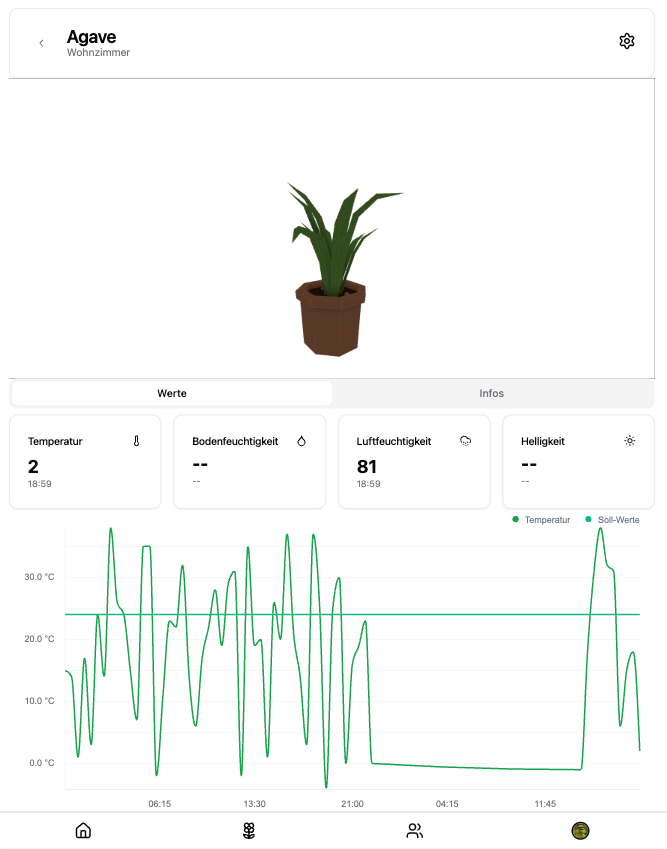
\includegraphics[scale=.5]{"./Umsetzung/images/sensora.png"}
	\caption{SinglePlantView in Aktion}
	\label{fig:SingelPlantView}
\end{figure}

Im oberen Abschnitt ist die Komponente \texttt{NavCard.vue} zu finden. Die ist für Überschriften mit einfacher Navigation zuständig in mehreren Views. Dieser Bereich ist durch die statische Anzeige des Pflanzennamens („Agave“) sowie der Rauminformation („Wohnzimmer“) gekennzeichnet. Diese Informationen werden direkt aus dem zentralen Datenmodell geladen, welches über ein Pinia-Store-Modul eingebunden ist. Der Benutzer erhält hier sofort kontextuelle Informationen zur Zuordnung der Pflanze im System.

Unmittelbar darunter befindet sich die 3D-Visualisierung der Pflanze, welche als zentrales visuelles Element prominent dargestellt ist. Diese Visualisierung basiert auf einem in der Datei \texttt{plantAvatars.ts} definierten Pflanzenmodell, das auf Basis des Pflanzentyps dynamisch geladen wird. Die Komponente zur Darstellung selbst ist als \texttt{<plant3d />} eingebettet, wobei ein Canvas-Rendering mit \texttt{Three.js} verwendet wird. Die visuelle Präsentation trägt zur Gamification der Anwendung bei, indem sie die emotionale Bindung und Wiedererkennung der Pflanzen fördern soll \cite{Werbach2012}.

Darunter folgt ein horizontal geteilter Abschnitt mit zwei Tabs: „Werte“ und „Infos“. Der Reiter „Werte“ ist standardmäßig aktiv, was sich in der visuellen Hervorhebung des Tabs zeigt. Innerhalb dieses Tabs sind vier Kartenkomponenten (Card-Komponenten) zu erkennen, die jeweils einen Umweltsensorwert repräsentieren: Temperatur, Bodenfeuchtigkeit, Luftfeuchtigkeit und Helligkeit. Diese sind als wiederverwendbare UI-Komponenten realisiert, die dynamisch Daten einlesen und anzeigen. Die Temperatur- und Luftfeuchtigkeitswerte sind im dargestellten Beispiel verfügbar („18 °C“ und „70 \%“), während Bodenfeuchte und Lichtstärke als nicht verfügbar („--“) markiert sind – ein Hinweis auf fehlerhafte oder fehlende Sensoranbindung. Jede Karte zeigt zusätzlich den letzten Messzeitpunkt, was eine präzise Einordnung der Datenqualität ermöglicht.

Der untere Teil der View wird durch die Verlaufsgraphen-Komponente dominiert, die in \texttt{PlantMeasuredValuesChart.vue} ausgelagert ist. Diese Komponente nutzt den Wrapper von \texttt{shadcn-vue} für \texttt{unovis}, um Messwerte über einen Zeitraum hinweg grafisch darzustellen. Im dargestellten Screenshot ist ein Temperaturliniendiagramm zu sehen, das über 24 Stunden  Werte anzeigt. Ein horizontaler Zielwert (Soll-Wert) ist ebenfalls dargestellt, was dem Benutzer eine sofortige Einschätzung der Umweltbedingungen erlaubt. Die Auswahl dieses Visualisierungsformats folgt dem Prinzip der kognitiven Entlastung: Durch einfache visuelle Kodierung können Zustände schneller interpretiert werden als durch numerische Tabellen.

Abgeschlossen wird die Komponente durch die \texttt{BottomNavBar.vue}, die über vier Icons eine einfache Navigation innerhalb der Anwendung ermöglicht. Diese sind als feste UI-Komponenten realisiert, wobei ein Button speziell dem Rücksprung zur Pflanzenübersicht oder der Startseite dient.

Insgesamt ergibt sich aus dieser strukturierten Aufteilung ein konsistentes, nutzerzentriertes Interface, das sowohl eine einfache Übersicht als auch eine tiefgehende Analyse einzelner Pflanzendaten erlaubt. Die klare funktionale Trennung – Datenanzeige oben, Visualisierung unten, Navigation ganz unten – folgt bewährten Usability-Prinzipien, die sich in wissenschaftlicher Literatur zur Mensch-Computer-Interaktion vielfach bewährt haben \cite{norman2013design}.



	\section{Benutzerzentriertes Design und UI/UX im Frontend}

Im Bezug auf die theoretische Erläuterung zentraler Konzepte wie \ac{UCD} und den Usability-Heuristiken nach Nielsen sowie dem \ac{UX}-Leitbild des Responsive Designs, wird in diesem Abschnitt die konkrete Umsetzung dieser Prinzipien im Rahmen der Vue.js-basierten Anwendung dargestellt. Ziel ist es, die Überführung theoretischer Vorgaben in praktische Gestaltungslösungen nachvollziehbar zu machen und zu zeigen, wie benutzerzentrierte Entwicklung zur Verbesserung der \ac{UI}-Qualität beiträgt.

\subsection{Anwendung von UCD im smarten Bewässerungssystem}

Die Nutzerforschung erfolgte durch halbstrukturierte Interviews mit VertreterInnen der Zielgruppe (z.\,B. HobbygärtnerInnen, technikaffine Personen). Daraus wurden mehrere Personas abgeleitet, die unterschiedliche Nutzungsmotive wie einfache Bedienung, Transparenz von Sensordaten und Kooperation abbilden. 

Darauf aufbauend wurden Wireframes auf Papier entwickelt, welche die Informationsarchitektur und zentrale Navigationsstrukturen skizzierten. Diese papierbasierten Modelle wurden iterativ angepasst und mit ausgewählten Testpersonen diskutiert. Durch diese formative Evaluation konnte bereits vor der Implementierung auf zentrale Anforderungen reagiert werden.

Auf Basis des Nutzerfeedbacks wurde die Darstellung der Gruppenansicht verbessert. Konkret ergaben sich folgende Anforderungen: Die NutzerInnen wünschten sich eine übersichtliche Darstellung der Gruppen sowie die Möglichkeit, auf einfache Weise die MitgliederInnen einer Gruppe einzusehen, ohne dass zu viele Informationen gleichzeitig auf dem Bildschirm erscheinen. Um diese Bedürfnisse zu erfüllen, wurde die GroupsView als Card-Layout konzipiert.

Diese Card präsentiert auf den ersten Blick nur die wichtigsten Informationen einer Gruppe. Über den Titel oder dem Button können die NutzerInnen die Card bei Bedarf „ausklappen“. Wird der Button gedrückt, erweitert sich die Card dynamisch und zeigt alle zugehörigen MitgliederInnen an. Dies verbessert die Übersichtlichkeit, da nicht alle Details permanent sichtbar sind und die NutzerInnen selbst steuern können, wann sie vertiefte Informationen einsehen.

Besonders benutzerfreundlich ist die neue Lösung auch darin, dass, wenn nur eine einzige Gruppe vorhanden ist, diese Card bereits automatisch ausgeklappt dargestellt wird. Auf diese Weise entfällt ein unnötiger zusätzlicher Klick und der direkte Zugriff auf die Gruppendetails wird erleichtert – ein kleines Detail, das jedoch signifikant zur Verbesserung der User Experience beiträgt.

Eine weitere Optimierung ist auf der SingelPlantView gemacht worden.
Aufgrund Nutzerfeedbacks wurde eine horizontale Linie in das Diagramm integriert, um den Sollwert des Messsatzes optisch darzustellen. Die Linie ermöglicht es den Nutzerinnen und Nutzern sofort zu erkennen, wo sich der Sollwert im Vergleich zu den aktuellen Messwerten befindet, sodass Abweichungen zwischen Soll- und Ist-Werten intuitiv nachvollziehbar werden. Dadurch wird nicht nur die Übersicht verbessert, sondern auch die Entscheidungsfindung optimiert, da eine klare visuelle Referenz bereitgestellt wird, anhand derer schneller und fundierter bestimmt werden kann, ob und in welchem Umfang eine Anpassung – beispielsweise im Bewässerungsprozess – erforderlich ist.

Durch die Integration der horizontalen Linie wird die Anwendung benutzerfreundlicher und nachvollziehbarer gestaltet. Gleichzeitig fügt sich die Linie nahtlos in das bestehende Design der SinglePlantView ein, das auf eine klare und konsistente Visualisierung von Daten setzt und damit zentrale Usability-Heuristiken wie die „Sichtbarkeit des Systemstatus“ sowie „Konsistenz und Standards“ unterstützt.


\subsection{Verwendete Heuristiken in der Anwendung}

Im Rahmen der konkreten Umsetzung wurden mehrere der zehn Usability-Heuristiken nach Nielsen gezielt berücksichtigt und systematisch in die Gestaltung der Benutzeroberfläche integriert:

Die Heuristik der Sichtbarkeit des Systemstatus wird durch die Verwendung von Toast-Notifications umgesetzt. Diese erscheinen automatisch bei allen Backend-Abfragen und informieren die NutzerInnen unmittelbar über den Verlauf und das Ergebnis einer Operation. Zusätzlich zeigen Statusindikatoren den Zustand des Sensors an.

Konsistenz und Standards werden durch den Einsatz von Tailwind CSS in Verbindung mit einheitlich definierten Designvariablen gewährleistet. Farben wie \texttt{primary}, \texttt{secondary}, \texttt{destructive} oder \texttt{background} kommen konsistent in Buttons, Karten und Formularen zum Einsatz und tragen zu einem kohärenten Erscheinungsbild bei \cite{TailwindCSS}.

Zur Umsetzung der Heuristik Fehlervorbeugung wurden alle Formulare mit clientseitiger Validierung ausgestattet. Eingaben werden bereits vor dem Absenden überprüft und Fehler mit Toast-Notifications angezeigt. Leere Eingabefelder enthalten stets einen Platzhalter, der die erwartete Eingabe beschreibt und so die korrekte Nutzung unterstützt.

Die Heuristik Hilfe und Dokumentation wurde durch einige kontextabhängige Tooltips sowie strukturierte Leere-Zustandsanzeigen berücksichtigt. Diese informieren über die nächsten Schritte oder ermöglichen eine direkte Navigation zur entsprechenden Aktion.

Ergänzend wurde auch die Heuristik Entsprechung zwischen System und realer Welt umgesetzt. Die hierarchische Struktur der Anwendung – von der Wohnung über Zimmer bis zu einzelnen Pflanzen – entspricht einem mentalen Modell aus dem Alltagskontext. Diese logische Ordnung fördert die Orientierung und trägt zu einer intuitiven Navigation bei.

Weitere Heuristiken wie Ästhetisches und minimalistisches Design sind durch das reduzierte Tailwind-basierte UI implizit realisiert worden.

Insgesamt zeigt sich, dass zentrale Usability-Prinzipien systematisch in das UI-Design integriert wurden, um eine benutzerfreundliche und robuste Anwendungserfahrung zu gewährleisten.

\subsection{Responsive Design}

Die Umsetzung des Responsive Designs wurde dabei so angelegt, dass die Anwendung unabhängig von der verwendeten Gerätegröße ein konsistentes und nutzerfreundliches Erlebnis bietet. Mithilfe der Tailwind-Breakpoints \texttt{sm}, \texttt{md}, \texttt{lg} und \texttt{xl} können Layout, Typografie und Abstände flexibel an kleinere, mittlere und größere Displays angepasst werden \cite{TailwindCSS}. Dies stellt sicher, dass die einzelnen Interface-Elemente, wie Buttons, Karten und Navigationsmenüs, sich dynamisch skalieren und neu anordnen, um eine optimale Lesbarkeit und Bedienbarkeit zu gewährleisten.

Für alle Gerätetypen wurde zudem eine Bottom-Navigation implementiert, die insbesondere auf mobilen Endgeräten eine intuitive und leicht zugängliche Navigation ermöglicht. Diese Navigation dient als zentrales Steuerelement, das es den NutzerInnen erlaubt, unkompliziert zwischen den Hauptbereichen der Anwendung zu wechseln, ohne auf aufwendige und unübersichtliche Menüstrukturen zurückgreifen zu müssen.

Ein weiteres Gestaltungselement ist das horizontale Scrollen auf der Startseite. Dieses Feature wurde eingeführt, um mehrere Informationskarten kompakt darzustellen, ohne dass der vertikale Platz unnötig beansprucht wird. Durch diese Anordnung können NutzerInnen schnell einen Überblick über verschiedene Inhalte erhalten und bei Bedarf mittels horizontaler Gesten zusätzliche Details abrufen. Insgesamt trägt das responsive Design dazu bei, dass die Anwendung sich flexibel an die individuellen Bedürfnisse und Nutzungsszenarien der AnwenderInnen anpasst und ein nahtloses Nutzungserlebnis über alle Geräte hinweg gewährleistet.

\subsection{User-Stories und funktionale Umsetzung}

Zur nutzerzentrierten Anforderungsdefinition wurden User-Stories eingesetzt, etwa:
\begin{itemize}
	\item \enquote{Als Benutzer möchte ich ein Pflanzenbild hochladen, damit die Pflanze automatisch erkannt wird.}
	\item \enquote{Als Benutzer möchte ich auch Mitglied anderer Gruppeen sein, um gemeinsam mit anderen NutzerInnen Pflanzen zu pflegen.}
\end{itemize}
Diese flossen in die Entwicklung dedizierter Komponenten ein (z.\,B. UploadPhotoView, GroupsView) und sicherten eine nutzergeleitete Gestaltung.

\section{Erweiterte Frontend-Techniken}
\label{sec:frontend-erweitert}

Im Folgenden werden ausgewählte Techniken vorgestellt, die in modernen Front\-end-Ar\-chi\-tek\-tur\-en zum Einsatz kommen. Einige dieser Methoden, wie Lazy Loading und Performance-Audits, wurden im Rahmen dieser Arbeit bereits angewendet. Andere Techniken, wie automatisierte Tests, werden exemplarisch vorgestellt, jedoch im Rahmen dieses \ac{POC} nicht implementiert.

\subsection{Lazy Loading in der Anwendung}

Zur Optimierung der initialen Ladezeit wurde in der entwickelten \ac{SPA} aktiv \emph{Lazy Loading} eingesetzt. Durch die dynamische Einbindung von Komponenten beim Navigieren zwischen Routen konnte die Bundle-Größe signifikant reduziert und die Interaktivität der Anwendung beschleunigt werden. 

Ein Beispiel für Lazy Loading stellt die dynamisch eingebundene Route zur Detailansicht einer Pflanze dar. Die zugehörige View \texttt{SinglePlantView.vue} wird erst bei tatsächlichem Aufruf geladen:

\begin{lstlisting}[caption=Lazy Loading per Route in Vue Router]
	routes: [
		{
			path: '/plant/:id',
			name: 'plantX',
			component: () => import('../views/SinglePlantView.vue'),
			meta: { requiresAuth: true, title: 'title.plant' },
		}
	]
\end{lstlisting}

Dieses Prinzip wurde konsistent auf alle Unterseiten angewendet. Der verwendete Build-Tool \emph{Vite} unterstützt dabei automatisch Code-Splitting und Tree Shaking, wodurch überflüssiger Code im Produktionsbuild entfernt wird \cite{ViteDocs2024,RollupDocs2024}.

\subsection{Frontend-Messung mit Lighthouse}

Zur Bewertung der Qualität der entwickelten Anwendung wurden regelmäßig \emph{Lighthouse-Audits} durchgeführt. Diese wurden in den Chrome Developer Tools erzeugt und analysierten zentrale Metriken wie \cite{GoogleLighthouse2024}:

\begin{itemize}
	\item \textbf{Performance:} First Contentful Paint, Time to Interactive, Speed Index
	\item \textbf{Accessibility:} Farbkontraste, semantische Struktur, ARIA-Rollen
	\item \textbf{Best Practices:} Ressourcennutzung, HTTPS
	\item  \textbf{SEO:}  Meta-Tags
\end{itemize}

Diese Angaben, wurden genutzt um stetig die Anwendung zu verbessern, gleich auch wenn bei einem \ac{POC} nicht der Schwerpunkt auf \ac{SEO} oder Accessability liegt. Die Performance wird auf den verschieden Seiten teilweise sehr unterschiedlich bewertet, da aber keine starken Verzögerungen bei der Bedienung identifiziert wurden, wurde keine allgemeine Optimierung durchgeführt.
	
	\newpage

	
	% ------------- Ende Hautpteil -------------
	
	\chapter{Kritische Reflexion}
	\section{Reflexion zur Frontend-Umsetzung}

Die Umsetzung des Frontends im Rahmen dieses Projekts kann insgesamt als gelungen und stabil bewertet werden. Die Anwendung ist vollständig funktionsfähig und unterstützt sowohl die deutsche als auch die englische Sprache durch ein konsistentes Internationalisierungskonzept. Zusätzlich bietet das Interface die Auswahl zwischen einem Dark Mode und einem Light Mode, was zur Barrierefreiheit und zum Nutzungskomfort beiträgt.

Besonders hervorzuheben ist das moderne, einheitliche und visuell ansprechende Design, das konsequent auf aktuellen UI/UX-Prinzipien basiert. Durch die Integration von Gamification-Elementen wie individuellen Pflanzen-Avataren wurde die Nutzerbindung zusätzlich gestärkt. Die Verwendung bewährter Best Practices in der Frontend-Architektur sowie die Orientierung am Flux-Prinzip sorgen für einen klar strukturierten Datenfluss und eine effiziente Benutzerinteraktion.

Ein wesentlicher Aspekt der Frontend-Gestaltung war die Gewährleistung eines flüssigen Nutzererlebnisses durch intuitive Navigation und konsistente Layouts. Die modular aufgebaute Komponentenstruktur ermöglicht eine gute Wartbarkeit und einfache Erweiterbarkeit der Anwendung.

\subsection{Verbesserungspotential}

Trotz der grundsätzlich hohen Qualität bestehen einige Optimierungsmöglichkeiten. Zum einen könnten Performance-Verbesserungen vorgenommen werden, um die Ladezeiten insbesondere bei datenintensiven Ansichten zu verringern. Zum anderen wurden einige Zusatzfunktionen aus zeitlichen Gründen nicht realisiert, die in einer späteren Entwicklungsphase ergänzt werden können.

Darüber hinaus sind drei kleinere Bugs bekannt, die zum aktuellen Stand noch nicht behoben wurden:

\begin{itemize}
	\item Auf Geräten ab der Android API Version 35 kann es bei aktivierter Drei-Punkte-Navigationsleiste zu einer Überlappung mit der App-eigenen Navigationsleiste kommen.
	\item Nach der Erstellung einer neuen Gruppe werden die darin enthaltenen Räume in der Bearbeitungsansicht nicht sofort angezeigt, sofern kein Seitenwechsel oder manueller Refresh erfolgt.
    \item Man bekommt einen Fehler, wenn man eine Pflanze bearbeitet, die einen fremden Controller hat, weil im Backend diese Änderungen nicht angenommen werde.
\end{itemize}

Diese Einschränkungen haben jedoch keinen kritischen Einfluss auf die Hauptfunktionen und Nutzbarkeit der Anwendung.

Bei einer Weiter Entwicklung des Frontends und damit auch bei einer realen Nutzung sollten Frontend-Test in Verbindung mit E2E-Tests durchgeführt werden. Dadurch können Funktionen überprüft und Bugs vermieden werden. 

\subsection{Fazit}

Die in der Konzeption formulierten Anforderungen an das Frontend wurden weitestgehend erfolgreich umgesetzt. Die Anwendung bietet ein modernes, benutzerfreundliches Interface mit internationaler Ausrichtung und ansprechendem Design. Funktionalität, Nutzerfluss und Wartbarkeit konnten auf hohem Niveau realisiert werden. Die identifizierten Verbesserungspunkte bieten darüber hinaus eine wertvolle Grundlage für zukünftige Weiterentwicklungen.
	%%Reflektiere über umsetzung der Komponenten, was hat gut funktioniert, was nicht, was war einfach, was war schwer, was war unerwartet, was war nicht so gut.
\section{IoT Device}
Das IoT Device wurde von einer Person als Hauptentwickler und mehreren Unterstützenden Entwicklern erstellt.
    \subsection{Hardware}:
    Geplant war das IoT Device als ein Gerät, das die Luftfeuchtigkeit und Temperatur misst und diese Daten an einen Server sendet.
    Für die Hardware wurde ein fertiger Bausatz von Alibaba gekauft, der alle benötigten Komponenten enthielt. Damit war es möglich, die Hardware schnell zusammenzubauen und zu testen.
    Die Sensoren sind nur mittelmäßig genau, was aber für ein Proof of Concept ausreichend ist.
    \subsection{Software}:
    Die Software wurde in C entwickelt. Dabei wurde CLion mit CMake als IDE verwendet.
    Dadurch kam es zu komplikationen im Setup, da die IDE nicht richtig konfiguriert war. Daraus resultierten verzögerungen die das Projekt belasteten
    Mehr feste Entwickler hätten hier helfen können.

Insgesamt lief die Entwicklung des IoT Devices gut, aber es gab einige Herausforderungen, die bewältigt werden mussten.
    Die Hardware war einfach zusammenzubauen, aber die Software war schwieriger zu implementieren als erwartet.
    Es gab einige Probleme mit der Kommunikation zwischen dem IoT Device und dem Server, die behoben werden mussten.
    Auch die Genauigkeit der Sensoren war nicht so hoch wie erhofft, was die Ergebnisse beeinflusste.
    Dennoch konnte das IoT Device erfolgreich entwickelt und getestet werden, und es erfüllt die Anforderungen des Projekts.
    
	
	\newpage 
	
	\chapter{Ausblick}
	\section{Reflexion zur Frontend-Umsetzung}

Die Umsetzung des Frontends im Rahmen dieses Projekts kann insgesamt als gelungen und stabil bewertet werden. Die Anwendung ist vollständig funktionsfähig und unterstützt sowohl die deutsche als auch die englische Sprache durch ein konsistentes Internationalisierungskonzept. Zusätzlich bietet das Interface die Auswahl zwischen einem Dark Mode und einem Light Mode, was zur Barrierefreiheit und zum Nutzungskomfort beiträgt.

Besonders hervorzuheben ist das moderne, einheitliche und visuell ansprechende Design, das konsequent auf aktuellen UI/UX-Prinzipien basiert. Durch die Integration von Gamification-Elementen wie individuellen Pflanzen-Avataren wurde die Nutzerbindung zusätzlich gestärkt. Die Verwendung bewährter Best Practices in der Frontend-Architektur sowie die Orientierung am Flux-Prinzip sorgen für einen klar strukturierten Datenfluss und eine effiziente Benutzerinteraktion.

Ein wesentlicher Aspekt der Frontend-Gestaltung war die Gewährleistung eines flüssigen Nutzererlebnisses durch intuitive Navigation und konsistente Layouts. Die modular aufgebaute Komponentenstruktur ermöglicht eine gute Wartbarkeit und einfache Erweiterbarkeit der Anwendung.

\subsection{Verbesserungspotential}

Trotz der grundsätzlich hohen Qualität bestehen einige Optimierungsmöglichkeiten. Zum einen könnten Performance-Verbesserungen vorgenommen werden, um die Ladezeiten insbesondere bei datenintensiven Ansichten zu verringern. Zum anderen wurden einige Zusatzfunktionen aus zeitlichen Gründen nicht realisiert, die in einer späteren Entwicklungsphase ergänzt werden können.

Darüber hinaus sind drei kleinere Bugs bekannt, die zum aktuellen Stand noch nicht behoben wurden:

\begin{itemize}
	\item Auf Geräten ab der Android API Version 35 kann es bei aktivierter Drei-Punkte-Navigationsleiste zu einer Überlappung mit der App-eigenen Navigationsleiste kommen.
	\item Nach der Erstellung einer neuen Gruppe werden die darin enthaltenen Räume in der Bearbeitungsansicht nicht sofort angezeigt, sofern kein Seitenwechsel oder manueller Refresh erfolgt.
    \item Man bekommt einen Fehler, wenn man eine Pflanze bearbeitet, die einen fremden Controller hat, weil im Backend diese Änderungen nicht angenommen werde.
\end{itemize}

Diese Einschränkungen haben jedoch keinen kritischen Einfluss auf die Hauptfunktionen und Nutzbarkeit der Anwendung.

Bei einer Weiter Entwicklung des Frontends und damit auch bei einer realen Nutzung sollten Frontend-Test in Verbindung mit E2E-Tests durchgeführt werden. Dadurch können Funktionen überprüft und Bugs vermieden werden. 

\subsection{Fazit}

Die in der Konzeption formulierten Anforderungen an das Frontend wurden weitestgehend erfolgreich umgesetzt. Die Anwendung bietet ein modernes, benutzerfreundliches Interface mit internationaler Ausrichtung und ansprechendem Design. Funktionalität, Nutzerfluss und Wartbarkeit konnten auf hohem Niveau realisiert werden. Die identifizierten Verbesserungspunkte bieten darüber hinaus eine wertvolle Grundlage für zukünftige Weiterentwicklungen.
	%% Hier bisschen Tagträumen was in Zukunft noch so kommen könnte.
\section{IoT Device}
Das IoT Device könnte in Zukunft durch bessere Sensoren und eine bessere Software weiter verbessert werden.
Mehr Modularität könnte auch helfen, das IoT Device einfacher zu erweitern und anzupassen.
Das IoT Device könnte auch in Zukunft durch eine bessere Benutzeroberfläche und eine bessere Integration in andere Systeme weiter verbessert werden.
	
	\newpage
	
	%------------- Literaturverzeichnis -------------
	\newpage
	\pagestyle{fancy}
	\fancyhead[R]{LITERATUR}

	%\chapter*{Literaturverzeichnis}
	\addcontentsline{toc}{chapter}{Literaturverzeichnis}
	\printbibliography
	\newpage

	%------------- Anhang -------------
	\cleardoublepage
	%\fancyhead[R]{ANHANG}

	%\chapter*{Anhang}
	%\addcontentsline{toc}{chapter}{Anhang}

	% Hier Anhänge einfügen:
	%\input{./Anhang/sensorwerte}
	%\input{./Anhang/schaltplan}

\newpage

	
\end{document}
